\documentclass[12pt]{article}
%
\usepackage{abstract,amsmath,amssymb,latexsym}
\usepackage{enumitem,epsf}
\usepackage{fullpage,tikz,float}
\usepackage[numbers]{natbib}
\usepackage[pdftex,colorlinks]{hyperref}

% locally defined macros
\usepackage{macros}

%%%%%%%%%%%%%%%%%%%%%%%%%%%%%%%%%%%%%%%%%%%%%%%%%%%%%%%%%%%%%

% Use the following for revealing TODOs and appendices
% Options are: \draftfalse or \drafttrue
\newif\ifdraft
\draftfalse

%%%%%%%%%%%%%%%%%%%%%%%%%%%%%%%%%%%%%%%%%%%%%%%%%%%%%%%%%%%%%

\title{
 \begin{minipage}[c]{1.05\textwidth}
 	\centerline{Toward Deeper Understanding of Neural Networks:}
 	\centerline{The Power of Initialization and a Dual View on Expressivity}
 \end{minipage}
}

\author{
	\vspace{1cm}
  Amit Daniely\thanks{Email: amitdaniely@google.com} \and
  Roy Frostig\thanks{Email: rf@cs.stanford.edu. Work performed at Google.} \and
  Yoram Singer\thanks{Email: singer@google.com}
}

\begin{document}

\maketitle
\thispagestyle{empty}

%% \vspace{-4cm}
%% \vspace*{\fill} {
%% \renewcommand{\abstractnamefont}{\normalfont\large\bfseries}
%% \renewcommand{\abstracttextfont}{\normalfont\normalfont}
%% \renewcommand{\baselinestretch}{1.0}
\begin{abstract}
%% \vspace{-0.25cm}
Scaling Transformers to longer sequence lengths has been a major problem in the
last several years, promising to improve performance in language modeling and
high-resolution image understanding, as well as to unlock new applications in
code, audio, and video generation.
The attention layer is the main bottleneck in scaling to longer sequences, as
its runtime and memory increase quadratically in the sequence length.
\sysnameone~\citep{dao2022flashattention} exploits the asymmetric GPU memory
hierarchy to bring significant memory saving (linear instead of quadratic) and
runtime speedup (2-4$\times$ compared to optimized baselines), with no approximation.
However, \sysnameone is still not nearly as fast as optimized matrix-multiply
(GEMM) operations, reaching only 25-40\% of the theoretical maximum FLOPs/s.
We observe that the inefficiency is due to suboptimal work partitioning between
different thread blocks and warps on the GPU, causing either low-occupancy or
unnecessary shared memory reads/writes.
We propose \sysname, with better work partitioning to address these issues.
In particular, we (1) tweak the algorithm to reduce the number of non-matmul
FLOPs (2) parallelize the attention computation, even for a single head, across
different thread blocks to increase occupancy, and (3) within each thread block,
distribute the work between warps to reduce communication through shared memory.
These yield around 2$\times$ speedup compared to \sysnameone, reaching 50-73\% of the
theoretical maximum FLOPs/s on A100 and getting close to the efficiency of GEMM
operations.
We empirically validate that when used end-to-end to train GPT-style models,
\sysname reaches training speed of up to 225 TFLOPs/s per A100 GPU (72\% model
FLOPs utilization).\footnote{\sysname
  is available at \url{https://github.com/Dao-AILab/flash-attention}}

% models with up to 2$\times$ longer sequence length compared to \sysnameone, in the
% same amount of time, leading to better downstream performance.\footnote{\sysname
%   is available at \url{https://github.com/Dao-AILab/flash-attention}}

\end{abstract}
%% }
%% \vspace*{\fill}

\ifdraft
\newpage
\section{Flows for trees and uniform distributions}


ping

\textcolor{blue}{
\textbf{To-do list (sensitivity analysis):}
\begin{enumerate}
    \item Sensitivity analysis for regular trees and uniform distribution 
    \item Generalization for DAGs
    \item Generalization for non-uniform distributions
\end{enumerate}
}
\textcolor{orange}{
\textbf{To-do list (policy networks):}
\begin{enumerate}
    \item Anonymous
    \begin{enumerate}
        \item Balance is impossible for some pairs of pointed DAGs and reward functions
        \item Some characterization of rewards that are particularly hard to approximate
        \item Sequences, Multisets, Anonymous and non-anonymous graphs (directed and undirected) 
\item trade-off between invariances in the networks and built into the state graph    \end{enumerate}
    \item Non-anonymous
\end{enumerate}
    }

\textcolor{red}{
\textbf{To-do list (evaluation and diagnostic of GFLowNets):}
\begin{enumerate}
    \item Current evaluation protocols are crap (usually focus on covering modes rather than approximation). Doing the right thing is also computationally infeasible for larges state-spaces 
    \item Convergence diagnostic based on some estimate of $\delta$, leveraging our theorems in the first part of the paper
    \item some diagonose based on, e.g, the estimates we can get from $R$ based on the trajectory-balance loss (in equilibrium, should be path independent, i.e., a constant)
\end{enumerate}
}


\fi

\newpage
\thispagestyle{empty}

{\large
\topskip0pt
\vspace*{\fill}
\tableofcontents
\vspace*{\fill}
}

\newpage

\setcounter{page}{1}

\documentclass[11pt]{report}
\usepackage[margin=2cm]{geometry}
\usepackage{graphicx}
\usepackage{float}
\usepackage{times}
\usepackage{url}
\usepackage[dvipsnames]{xcolor}
\usepackage{hyperref}

\newcommand{\specialcell}[2][c]{\begin{tabular}[#1]{@{}c@{}}#2\end{tabular}}

\newcommand{\Gap}{\texorpdfstring{\hfill}{}}
\newcommand{\Rec}{\texorpdfstring{{\small\emph{\color{ccai-blue}{\fbox{High Leverage}}}}}{}}
\newcommand{\HighRisk}{\texorpdfstring{{\small\emph{\color{ccai-yellow-darker}{\fbox{Uncertain Impact}}}}}{}}
\newcommand{\Longterm}{\texorpdfstring{{\small\emph{\color{ccai-green}{\fbox{Long-term}}}}}{}}

\begin{document}

\begin{abstract}
Climate change is one of the greatest challenges facing humanity, and we, as machine learning experts, may wonder how we can help. Here we describe how machine learning can be a powerful tool in reducing greenhouse gas emissions and helping society adapt to a changing climate. From smart grids to disaster management, we identify high impact problems where existing gaps can be filled by machine learning, in collaboration with other fields. Our recommendations encompass exciting research questions as well as promising business opportunities. We call on the machine learning community to join the global effort against climate change.
\vskip .5in
\end{abstract}

\part*{Introduction}
The effects of climate change are increasingly visible.\footnote{For a layman's introduction to the topic of climate change, see \cite{romm2018climate, archer2010climate}.} Storms, droughts, fires, and flooding have become stronger and more frequent \cite{field2012managing}. Global ecosystems are changing, including the natural resources and agriculture on which humanity depends. The 2018 intergovernmental report on climate change estimated that the world will face catastrophic consequences unless global greenhouse gas emissions are eliminated within thirty years \cite{ipcc_global_2018}. Yet year after year, these emissions rise.

Addressing climate change involves mitigation (reducing emissions) and adaptation (preparing for unavoidable consequences). Both are multifaceted issues. Mitigation of greenhouse gas (GHG) emissions requires changes to electricity systems, transportation, buildings, industry, and land use. Adaptation requires planning for resilience and disaster management, given an understanding of climate and extreme events. Such a diversity of problems can be seen as an opportunity: there are many ways to have an impact.

In recent years, machine learning (ML) has been recognized as a broadly powerful tool for technological progress. Despite the growth of movements applying ML and AI to problems of societal and global good,\footnote{See the AI for social good movement (e.g.~\cite{hager2019artificial, berendt2019ai}), ML for the developing world~\cite{de2018machine}, the computational sustainability movement (e.g.~\cite{kelling2018computational, joppa2017case, lassig2016computational, gomes2009computational, dietterich2009machine}, the American Meteorological Society's Committee on AI Applications to Environmental Science, and the field of Climate Informatics (\url{www.climateinformatics.org}) \cite{Monteleoni2013chapter}, as well as the relevant survey papers \cite{faghmous2014big, kaack2019challenges, ford2016opinion}.} there remains the need for a concerted effort to identify how these tools may best be applied to tackle climate change. Many ML practitioners wish to act, but are uncertain how. On the other side, many fields have begun actively seeking input from the ML community.

This paper aims to provide an overview of where machine learning can be applied with high impact in the fight against climate change, through either effective engineering or innovative research. The strategies we highlight include climate mitigation and adaptation, as well as meta-level tools that enable other strategies. In order to maximize the relevance of our recommendations, we have consulted experts across many fields (see \hyperref[sec:acknowledgments]{{\small{Acknowledgments}}}) in the preparation of this paper.


\begin{table}
\begin{small}
\begin{center}
\begin{tabular}{l l l l l l l l l l l l}  \toprule
     \multicolumn{2}{l}{ }
         & \small{\rotatebox{90}{\parbox{2.2cm}{Causal\\inference}}}
         & \small{\rotatebox{90}{\parbox{2.2cm}{Computer\\vision}}}
         & \small{\rotatebox{90}{\parbox{2.2cm}{Interpretable\\models}}}
         & \small{\rotatebox{90}{NLP}}
         & \small{\rotatebox{90}{\parbox{2.2cm}{RL \& Control}}}
        %  & \small{\rotatebox{90}{Robotics}}
         & \small{\rotatebox{90}{\parbox{2.2cm}{Time-series analysis}}}
         & \small{\rotatebox{90}{\parbox{2.2cm}{Transfer\\learning}}}
         & \small{\rotatebox{90}{\parbox{2.2cm}{Uncertainty\\quantification}}}
         & \small{\rotatebox{90}{\parbox{2.2cm}{Unsupervised\\learning}}}
    \\ \midrule
    \rowcolor{ccai-blue-lightest}
    \multicolumn{2}{l}{1 \hyperref[sec:electricity-systems]{Electricity systems}} 
        & % Causal inf
        &  % Comp vision
        & % Interpretable ml
        & % nlp
        & % rl + control
        & % time series
        & % transfer
        & % UQ
        & \\% unsupervised \ref{sub
    & \hyperref[sec:electricity-lowCarbon]{Enabling low-carbon electricity}
        & % Causal inf
        & $\bullet$% Comp vision
        & $\bullet$% % Interpretable ml
        & % % nlp
        & $\bullet$%% rl + control
        & $\bullet$% % time series
        & % transfer
        & $\bullet$% % UQ
        & $\bullet$\\% unsupervised 
    & \hyperref[sec:electricity-currentSystemImpact]{Reducing current-system impacts}
        & % Causal inf
        & $\bullet$% Comp vision
        & % Interpretable ml
        & % nlp
        & % rl + control
        & $\bullet$% % time series
        & % transfer
        & $\bullet$% % UQ
        & $\bullet$\\% unsupervised 
    & \hyperref[sec:electricity-developing]{Ensuring global impact}
        & % Causal inf
        & $\bullet$% Comp vision
        & % Interpretable ml
        & % nlp
        & % rl + control
        & % time series
        & $\bullet$ % transfer
        & % UQ
        & $\bullet$\\% unsupervised 
    \rowcolor{ccai-blue-lightest}
    \multicolumn{2}{l}{2 \hyperref[sec:transportation]{Transportation}} 
        & % Causal inf
        & % Comp vision
        &% Interpretable ml
        & % nlp
        & % rl + control
        & % time series
        & % transfer
        & % UQ
        & \\% unsupervised 
    & \hyperref[sec:TReducing]{Reducing transport activity}
        & % Causal inf
        & $\bullet$% Comp vision
        & % Interpretable ml
        & % nlp
        & % rl + control
        & $\bullet$% time series
        & % transfer
        & $\bullet$% UQ
        & $\bullet$\\% unsupervised     
   & \hyperref[sec:TEfficient]{Improving vehicle efficiency}
        & % Causal inf
        & $\bullet$% Comp vision
        & % Interpretable ml
        & % nlp
        & $\bullet$% rl + control
        & % time series
        & % transfer
        & % UQ
        & \\% unsupervised    
   & \hyperref[sec:TFuels]{Alternative fuels \& electrification}
        & % Causal inf
        & % Comp vision
        & % Interpretable ml
        & % nlp
        & $\bullet$% rl + control
        & % time series
        & % transfer
        & % UQ
        & $\bullet$ \\% unsupervised    
   & \hyperref[sec:modalshift]{Modal shift}
        & $\bullet$% Causal inf
        & $\bullet$% Comp vision
        & % Interpretable ml
        & % nlp
        & % rl + control
        & $\bullet$% time series
        & % transfer
        & $\bullet$% UQ
        & \\% unsupervised    
    \rowcolor{ccai-blue-lightest}
    \multicolumn{2}{l}{3 \hyperref[sec:buildings-cities]{Buildings and cities}} 
        & % Causal inf
        & % Comp vision
        & % Interpretable ml
        & % nlp
        & % rl + control
        & % time series
        & % transfer
        & % UQ
        & \\% unsupervised 
    & \hyperref[sec:indv]{Optimizing buildings}
        & $\bullet$% Causal inf
        & % Comp vision
        & % Interpretable ml
        & % nlp
        & $\bullet$% rl + control
        & $\bullet$% time series
        & $\bullet$% transfer
        & % UQ
        & \\% unsupervised 
    & \hyperref[sec:distr]{Urban planning}
        & % Causal inf
        & $\bullet$% Comp vision
        & % Interpretable ml
        & % nlp
        & % rl + control
        & $\bullet$% time series
        & $\bullet$% transfer
        & % UQ
        & $\bullet$\\% unsupervised 
    & \hyperref[sec:cities]{The future of cities}
        & % Causal inf
        & % Comp vision
        & % Interpretable ml
        & $\bullet$%% nlp
        & % rl + control
        & %% time series
        & $\bullet$%% transfer
        & $\bullet$% UQ
        & $\bullet$\\% unsupervised 
    \rowcolor{ccai-blue-lightest}
    \multicolumn{2}{l}{4 \hyperref[sec:industry]{Industry}} 
        & % Causal inf
        & % Comp vision
        & % Interpretable ml
        & % nlp
        & % rl + control
        & % time series
        & % transfer
        & % UQ
        & \\% unsupervised 
    & \hyperref[sec:supplychains]{Optimizing supply chains}
        & % Causal inf
        & $\bullet$ %% Comp vision
        & % Interpretable ml
        & % nlp
        & $\bullet$ % rl + control
        & $\bullet$ % time series
        & % transfer
        & % UQ
        & \\% unsupervised 
    & \hyperref[sec:materialsandconstruction]{Improving materials}
        & %% Causal inf
        & % Comp vision
        & % Interpretable ml
        & % nlp
        & % rl + control
        & % time series
        & %% transfer
        & % UQ
        & $\bullet$ \\% unsupervised 
    & \hyperref[sec:demandresponse]{Production \& energy}
        & %% Causal inf
        & $\bullet$%% Comp vision
        & $\bullet$ %% Interpretable ml
        & % nlp
        & $\bullet$% rl + control
        & %% time series
        & %% transfer
        & % UQ
        & \\% unsupervised 
    \rowcolor{ccai-blue-lightest}
    \multicolumn{2}{l}{5 \hyperref[sec:afolu]{Farms \& forests}} 
        & % Causal inf
        & % Comp vision
        & % Interpretable ml
        & % nlp
        & % rl + control
        & % time series
        & % transfer
        & % UQ
        & \\% unsupervised 
    & \hyperref[sec:emissions-detection]{Remote sensing of emissions}
        & % Causal inf
        & $\bullet$% Comp vision
        & % Interpretable ml
        & % nlp
        & % rl + control
        & % time series
        & % transfer
        & % UQ
        & \\% unsupervised 
    & \hyperref[sec:agriculture]{Precision agriculture}
        & % Causal inf
        & $\bullet$% Comp vision
        & % Interpretable ml
        & % nlp
        & $\bullet$% rl + control
        & $\bullet$% time series
        & % transfer
        & % UQ
        & \\% unsupervised 
    & \hyperref[sec:peatlands]{Monitoring peatlands}
        & % Causal inf
        & $\bullet$% Comp vision
        & % Interpretable ml
        & % nlp
        & % rl + control
        & % time series
        & % transfer
        & % UQ
        & \\% unsupervised 
    & \hyperref[sec:forests]{Managing forests}
        & % Causal inf
        & $\bullet$% Comp vision
        & % Interpretable ml
        & % nlp
        & $\bullet$ % rl + control
        & $\bullet$ % time series
        & % transfer
        & % UQ
        & \\% unsupervised 
    \rowcolor{ccai-blue-lightest}
    \multicolumn{2}{l}{6 \hyperref[sec:ccs]{Carbon dioxide removal}}
        & % Causal inf
        & % Comp vision
        & % Interpretable ml
        & % nlp
        & % rl + control
        & % time series
        & % transfer
        & % UQ
        & \\
    & \hyperref[sec:ccs]{Direct air capture}
        & % Causal inf
        & % Comp vision
        & % Interpretable ml
        & % nlp
        & % rl + control
        & % time series
        & % transfer
        & % UQ
        & $\bullet$\\% unsupervised 
    & \hyperref[subsubsec: sequestrativervin]{Sequestering~\cd}
        & % Causal inf
        & $\bullet$% Comp vision
        & % Interpretable ml
        & % nlp
        & % rl + control
        & % time series
        & % transfer
        & $\bullet$% UQ
        & $\bullet$\\% unsupervised 
    \rowcolor{ccai-blue-lightest}
    \multicolumn{2}{l}{7 \hyperref[sec: climate prediction]{Climate prediction}} 
        & % Causal inf
        & % Comp vision
        & % Interpretable ml
        & % nlp
        & % rl + control
        & % time series
        & % transfer
        & % UQ
        & \\% unsupervised 
    & \hyperref[sec:climate-models-params]{Uniting data, ML \& climate science}
        & % Causal inf
        & $\bullet$% Comp vision
        & $\bullet$% Interpretable ml
        & % nlp
        & % rl + control
        & $\bullet$% time series
        & % transfer
        & $\bullet$% UQ
        & \\% unsupervised 
    & \hyperref[sec:models-extreme-events]{Forecasting extreme events}
        & % Causal inf
        & $\bullet$% Comp vision
        & $\bullet$% Interpretable ml
        & % nlp
        & % rl + control
        & $\bullet$% time series
        & % transfer
        & $\bullet$% UQ
        & \\% unsupervised 
    \rowcolor{ccai-blue-lightest}
    \multicolumn{2}{l}{8 \hyperref[sec:societal-impacts]{Societal impacts}} 
        & % Causal inf
        & % Comp vision
        & % Interpretable ml
        & % nlp
        & % rl + control
        & % time series
        & % transfer
        & % UQ
        & \\% unsupervised 
    & \hyperref[subsub:ecology]{Ecology}
        & % Causal inf
        & $\bullet$% Comp vision
        & % Interpretable ml
        & % nlp
        & % rl + control
        & % time series
        & $\bullet$% transfer
        & % UQ
        & \\% unsupervised 
    & \hyperref[subsub:infrastructure]{Infrastructure}
        & % Causal inf
        & % Comp vision
        & % Interpretable ml
        & % nlp
        & $\bullet$% rl + control
        & $\bullet$% time series
        & % transfer
        & $\bullet$% UQ
        & \\% unsupervised 
    & \hyperref[subsub:social_systems]{Social systems}
        & % Causal inf
        & $\bullet$% Comp vision
        & % Interpretable ml
        & % nlp
        & % rl + control
        & $\bullet$% time series
        & % transfer
        & % UQ
        & $\bullet$\\% unsupervised 
    & \hyperref[subsub:crisis]{Crisis}
        & % Causal inf
        & $\bullet$% Comp vision
        & % Interpretable ml
        & $\bullet$% nlp
        & % rl + control
        & % time series
        & % transfer
        & % UQ
        & \\% unsupervised 
    \rowcolor{ccai-blue-lightest}
    \multicolumn{2}{l}{9 \hyperref[sec:geoengineering]{Solar geoengineering}} 
        & % Causal inf
        & % Comp vision
        & % Interpretable ml
        & % nlp
        & % rl + control
        & % time series
        & % transfer
        & % UQ
        & \\% unsupervised 
    & \hyperref[subsub:better-aerosols]{Understanding \& improving aerosols}
        & % Causal inf
        & % Comp vision
        & % Interpretable ml
        & % nlp
        & % rl + control
        & $\bullet$% time series
        & % transfer
        & $\bullet$% UQ
        & \\% unsupervised 
    & \hyperref[subsub:planetary-control]{Engineering a planetary control system}
        & % Causal inf
        & % Comp vision
        & % Interpretable ml
        & % nlp
        & $\bullet$% rl + control
        & % time series
        & % transfer
        & $\bullet$% UQ
        & \\% unsupervised 
    & \hyperref[subsub:impact-models]{Modeling impacts}
        & % Causal inf
        & % Comp vision
        & % Interpretable ml
        & % nlp
        & % rl + control
        & $\bullet$% time series
        & % transfer
        & $\bullet$% UQ
        & \\% unsupervised 
    \rowcolor{ccai-blue-lightest}
    \multicolumn{2}{l}{10 \hyperref[sec:tools-individuals]{Individual action}} 
        & % Causal inf
        & % Comp vision
        & % Interpretable ml
        & % nlp
        & % rl + control
        & % time series
        & % transfer
        & % UQ
        & \\% unsupervised 
    & \hyperref[sec:personal_carbon_footprint]{Understanding personal footprint}
        & $\bullet$% Causal inf
        & % Comp vision
        & % Interpretable ml
        & $\bullet$% nlp
        & $\bullet$% rl + control
        & $\bullet$% time series
        & % transfer
        & % UQ
        & \\% unsupervised 
    & \hyperref[sec:behavior_change]{Facilitating behavior change}
        & % Causal inf
        & % Comp vision
        & % Interpretable ml
        & $\bullet$% nlp
        & % rl + control
        & % time series
        & % transfer
        & % UQ
        & $\bullet$\\% unsupervised 
    \rowcolor{ccai-blue-lightest}
    \multicolumn{2}{l}{11 \hyperref[sec:toolsforsociety]{Collective decisions}} 
        & % Causal inf
        & % Comp vision
        & % Interpretable ml
        & % nlp
        & % rl + control
        & % time series
        & % transfer
        & % UQ
        &  \\% unsupervised 
    & \hyperref[sec:coordination]{Modeling social interactions}
        & % Causal inf
        & % Comp vision
        & $\bullet$ % Interpretable ml
        & % nlp
        & $\bullet$ % rl + control
        & % time series
        & % transfer
        & % UQ
        & \\% unsupervised 
    & \hyperref[sec:decisionmaking]{Informing policy}
        & $\bullet$ % Causal inf
        & $\bullet$ % Comp vision
        & % Interpretable ml
        & $\bullet$% nlp
        & % rl + control
        & % time series
        & % transfer
        & $\bullet$% UQ
        & $\bullet$\\% unsupervised 
    & \hyperref[subsec:markets]{Designing markets}
        & % Causal inf
        & % Comp vision
        & % Interpretable ml
        & % nlp
        & $\bullet$% rl + control
        & $\bullet$% time series
        & % transfer
        & % UQ
        & $\bullet$\\% unsupervised 
    \rowcolor{ccai-blue-lightest}
    \multicolumn{2}{l}{12 \hyperref[sec:education]{Education}} 
        & % Causal inf
        & % Comp vision
        & % Interpretable ml
        & $\bullet$% nlp
        & $\bullet$% rl + control
        & % time series
        & % transfer
        & % UQ
        & \\% unsupervised 
    \rowcolor{ccai-blue-lightest}
    \multicolumn{2}{l}{13 \hyperref[sec:finance]{Finance}} 
        & % Causal inf
        & % Comp vision
        & % Interpretable ml
        & $\bullet$% nlp
        & % rl + control
        & $\bullet$% time series
        & % transfer
        & $\bullet$% UQ
        & \\% unsupervised 
    \bottomrule
\end{tabular}
\caption{Climate change solution domains, corresponding to sections of this paper, matched with selected areas of ML that are relevant to each. }
\label{tab:summary}
\end{center}
\end{small}
\end{table}


\subsection*{Who is this paper written for?}

We believe that our recommendations will prove valuable to several different audiences (detailed below). In our writing, we have assumed some familiarity with basic terminology in machine learning, but do not assume any prior familiarity with application domains (such as agriculture or electric grids).\\

\textbf{Researchers and engineers:}
We identify many problems that require conceptual innovation and can advance the field of ML, as well as being highly impactful. For example, we highlight how climate models afford an exciting domain for interpretable ML (see \S\ref{sec: climate prediction}).
We encourage researchers and engineers across fields to use their expertise in solving urgent problems relevant to society.\\

\textbf{Entrepreneurs and investors:} We identify many problems where existing ML techniques could have a major impact without further research, and where the missing piece is deployment. We realize that some of the recommendations we offer here will make valuable startups and nonprofits. For example, we highlight techniques for providing fine-grained solar forecasts for power companies (see \S\ref{sec:electricity-lowCarbon}), tools for helping reduce personal energy consumption (see \S\ref{sec:behavior_change}), and predictions for the financial impacts of climate change (see \S\ref{sec:finance}). We encourage entrepreneurs and investors to fill what is currently a wide-open space.\\

\textbf{Corporate leaders:} We identify problems where ML can lead to massive efficiency gains if adopted at scale by corporate players. For example, we highlight means of optimizing supply chains to reduce waste (see \S\ref{sec:supplychains}) and software/hardware tools for precision agriculture (see \S\ref{sec:agriculture}). We encourage corporate leaders to take advantage of opportunities offered by ML to benefit both the world and the bottom line.\\

\textbf{Local and national governments:} We identify problems where ML can improve public services, help gather data for decision-making, and guide plans for future development. For example, we highlight intelligent transportation systems (see \S\ref{sec:modalshift}), techniques for automatically assessing the energy consumption of buildings in cities (see \S\ref{sec:indv}),
and tools for improving disaster management (see \S\ref{subsub:crisis}). We encourage governments to consult ML experts while planning infrastructure and development, as this can lead to better, more cost-effective outcomes. We further encourage public entities to release data that may be relevant to climate change mitigation and adaptation goals.\\

\subsection*{How to read this paper} \label{sub:howtoread}
The paper is broken into sections according to application domain (see Table \ref{tab:summary}). To help the reader, we have also included the following flags at the level of individual strategies.
\begin{itemize}
\item \textbf{\Rec} $\,$ denotes bottlenecks that domain experts have identified in climate change mitigation or adaptation and that we believe to be particularly well-suited to tools from ML. These areas may be especially fruitful for ML practitioners wishing to have an outsized impact, though applications not marked with this flag are also valuable and should be pursued.
\item \textbf{\Longterm} $\,$ denotes applications that will have their primary impact after 2040. While extremely important, these may in some cases be less pressing than those which can help act on climate change in the near term.
\item \textbf{\HighRisk} $\,$ denotes applications where the impact on GHG emissions is uncertain (for example, the \emph{Jevons paradox} may apply\footnote{The Jevons paradox in economics refers to a situation where increased efficiency nonetheless results in higher overall demand. For example, autonomous vehicles could cause people to drive far more, so that overall GHG emissions could increase even if each ride is more efficient. In such cases, it becomes especially important to make use of specific policies, such as carbon pricing, to direct new technologies and the ML behind them. See also the literature on rebound effects and induced demand.}) or where there is  potential for undesirable side effects (\emph{negative externalities}).
\end{itemize}

These flags should not be taken as definitive; they represent our understanding of more rigorous analyses within the domains we consider, combined with our subjective evaluation of the potential role of ML in these various applications.

Despite the length of the paper, we cannot cover everything. There will certainly be many applications that we have not considered, or that we have erroneously dismissed. We look forward to seeing where future work leads.

\subsection*{A call for collaboration}

All of the problems we highlight in this paper require collaboration across fields. As the language used to refer to problems often varies between disciplines, we have provided keywords and background reading within each section of the paper. Finding collaborators and relevant data can sometimes be difficult; for additional resources, please visit the website that accompanies this paper: \url{https://www.climatechange.ai/}.

Collaboration makes it easier to develop effective strategies. Working with domain experts reduces the chance of using powerful tools when simple tools will do the job, of working on a problem that isn't actually relevant to practitioners, of overly simplifying a complex issue,
or of failing to anticipate risks.

Collaboration can also help ensure that new work reaches the audience that will use it. To be impactful, ML code should be accessible and published using a language and a platform that are already popular with the intended users. For maximal impact, new code can be integrated into an existing, widely used tool.

We emphasize that machine learning is not a silver bullet. The applications we highlight are impactful, but no one solution will ``fix'' climate change. There are also many areas of action where ML is inapplicable, and we omit these entirely. Furthermore, technology alone is not enough -- technologies that would address climate change have been available for years, but have largely not been adopted at scale by society. While we hope that ML will be useful in reducing the costs associated with climate action, humanity also must decide to act.

\end{document}

%!TEX root = ../main.tex

\section{Related Work}
\label{sec:related}

\textbf{State space models} have shown promise in modeling sequential data, including time series data~\citep{gu2022efficiently}, audio~\citep{goel2022s}, and visual data~\citep{nguyen2022s4nd}.
Our model builds off work on simplifying and parameterizing diagonal versions of S4~\citep{gu2022parameterization,gupta2022diagonal, gu2022train}.
Gated state spaces~\citep{mehta2022long} also aim to adapt SSMs to language modeling, but our results suggest that the GSS model does not perform as well as \hthree (or even as well as earlier SSMs like S4D).
The idea to combine SSMs with attention in hybrid models is not new; Mehta et al.~\citep{mehta2022long} also showed that interleaving attention with their GSS layer can improve performance, which we also validate on our OpenWebText experiments.
These positive results suggest that attention and SSMs are complementary, and that hybrid models may be a promising direction for future work.

\textbf{Large language foundation models}~\citep{bommasani2021opportunities} have demonstrated the power of scaling attention-based networks to billions of parameters and training them on trillions of tokens~\citep{hoffmann2022training}.
Understanding the mechanistic basis~\citep{elhage2021mathematical} behind these models may yield insights into better design choices for future models.
These and similar explorations have informed the design of \hthree and our selection of synthetic languages.
A number of recent works have also explored how to address the shortcomings of attention by approximating the attention computation~\citep{wang2020linformer,katharopoulos2020transformers, choromanski2020rethinking,tay2020long, kitaev2020reformer, daras2020smyrf}.
We believe these efforts are complementary to SSMs, and we are excited to see how they can be combined in future work.

\textbf{Linear attention}~\citep{katharopoulos2020transformers} and classical sequence models like RNNs serve as inspiration for \hthree.
Appendix~\ref{app:linear_attention} draws a direct connection between linear attention and LTI systems.
Luo et al.~\citep{luo2021stable} also propose a variant of linear attention that can achieve $O(n \log n)$ scaling in sequence length.
Appendix~\ref{sec:app_additional_experiments} evaluates linear attention on language modeling, and finds that it underperforms exact attention, whereas \hthree outperforms attention.
The multiplicative interactions in \hthree are reminiscent of gating mechanisms in LSTMs~\citep{hochreiter1996lstm} and GRUs~\citep{cho2014properties}, which suggests that architectural lessons from these sequence models may be useful for adapting SSMs to language modeling.
A number of algorithms for scaling attention to longer sequences have also been proposed, such as Transformer-XL~\citep{dai2019transformer}, Reformer~\citep{kitaev2020reformer}, Performer~\citep{choromanski2020rethinking}, and Perceiver AR~\citep{hawthorne2022general}.
Some of these approaches underperform exact attention on language modeling, and may be slower in wall-clock speed~\citep{dao2022flashattention}.
A thorough comparison of these alternatives to exact attention and how well they scale in model size and amount of training data is fruitful future work.

\textbf{FFT} algorithms are used in a wide variety of applications, including signal processing~\citep{oppenheim1978applications}, control theory~\citep{brogan1974modern}, and more.
Various algorithms for computing the FFT have existed for decades~\citep{oppenheim2001discrete}.
We hope our work on appealing to these classic algorithms to accelerate new applications such as learned SSMs will inspire future algorithmic exploration, even if hardware is not designed for them~\citep{hooker2021hardware}.

%%% Local Variables:
%%% mode: latex
%%% TeX-master: "../main"
%%% End:

\section{Setting}

\paragraph{Notation.} We denote
%% scalars by lowercase and uppercase letters and (e.g., $x, X$),
vectors by bold-face letters (e.g.\ $\x$), and
matrices by upper case Greek letters (e.g.\ $\Sigma$). The $2$-norm of $\x
\in \reals^d$ is denoted by $\|\x\|$. For functions $\sigma:\reals\to\reals$
we let
$$
\|\sigma\| \textstyle
	:=\sqrt{\E_{X\sim\cn(0,1)}\sigma^2(X)}
	\; = \sqrt{\frac{1}{\sqrt{2\pi}}
		\int_{-\infty}^\infty \sigma^2(x)e^{-\frac{x^2}{2}}dx} \,.
$$
%
Let $G=(V,E)$ be a directed acyclic graph. The set of neighbors incoming to
a vertex $v$ is denoted $\IN(v):=\{u\in V\mid uv\in E\}$.
%% The $d$ dimensional vector space of the reals is denoted by
%% $\reals^d$.
The $d-1$ dimensional sphere is denoted $\sphere^{d-1} =
\{\x\in\reals^d \mid \|\x\|=1\}$. We provide a brief overview of
reproducing kernel Hilbert spaces in the sequel and merely introduce
notation here. In a Hilbert space $\ch$, we use a slightly
non-standard notation $\ch^B$ for the ball of radius $B$, $\{\x \in
\ch \mid \|\x\|_\ch \leq B\}$. We use $[x]_+$ to denote $\max(x,0)$
and $\ind[b]$ to denote the indicator function of a binary variable
$b$.

\paragraph{Input space.} Throughout the paper we assume that each example is
a sequence of $n$ elements, each of which is represented as a unit vector. 
Namely, we fix $n$ and take the input space to be
	$\cx=\cx_{n,d}=\left(\sphere^{d-1}\right)^n$.
Each input example is denoted,
\begin{align} \label{eq:coordinates}
	\x=(\x^1,\ldots,\x^n), ~\textwhere \x^i\in \sphere^{d-1} \,.
\end{align}
%
We refer to each vector $\x^i$ as the input's $i$th {\em
  coordinate}, and use $x^i_{j}$ to denote it $j$th scalar
entry. Though this notation is slightly non-standard, it unifies 
input types seen in various domains. For example,
binary features can be encoded by taking $d=1$, in which case
$\cx=\{\pm 1\}^n$. Meanwhile, images and audio signals are often
represented as bounded and continuous numerical values---we can assume
in full generality that these values lie in $[-1,1]$. To match the setup
above, we embed $[-1,1]$ into the circle $\sphere^1$, e.g.\ via the map $x
\mapsto \left(\sin\left(\frac{\pi x}{2}\right), \cos\left(\frac{\pi
  x}{2}\right)\right)$. When each coordinate is categorical---taking
one of $d$ values---we can represent category $j\in[d]$ by the unit
vector $\mathbf e_j\in\sphere^{d-1}$. When $d$ may be very large or
the basic units exhibits some structure, such as when the input is a sequence
of words, a more concise encoding may be
useful, e.g.\ as unit vectors in a low dimension space $\sphere^{d'}$
where $d'\ll d$ (see for
instance~\citet{mikolov2013distributed,levy2014neural}).

\paragraph{Supervised learning.} The goal in supervised learning is to
devise a mapping from the input space $\cx$ to an output space $\cy$ based on a sample
$S=\{(\x_1,y_1),\ldots,(\x_m,y_m)\}$, where $(\x_i,y_i)\in\cx\times\cy$, 
drawn i.i.d.\ from a distribution $\cd$ over $\cx\times\cy$.
%
A supervised learning problem is further specified by an output length $k$ and a loss function
$\ell : \reals^k \times \cy \to [0,\infty)$, and the goal is to find a
predictor $h:\cx\to\reals^k$ whose loss,
$\cl_{\cd}(h) := \E_{(\x,y)\sim\cd} \ell(h(\x),y)$, is small.
%
The {\em empirical} loss $\cl_{S}(h):= \frac 1 m \sum_{i=1}^m
\ell(h(\x_i),y_i)$ is commonly used as a proxy for the loss
$\cl_{\cd}$.
%
Regression problems correspond to $\cy=\reals$ and, for
instance, the squared loss $\ell(\hat y,y)=(\hat y -y)^2$.
%
Binary classification is captured by $\cy=\{\pm 1\}$ and, say, the
zero-one loss $\ell(\hat y,y)= \ind[\hat y y \leq 0]$ or the hinge
loss $\ell(\hat y,y)=[1-\hat y y]_+$, with standard extensions to the
multiclass case.
A loss $\ell$ is $L$-Lipschitz if $|\ell(y_1,y) - \ell(y_2,y) | \leq L
|y_1 - y_2|$ for all $y_1,y_2 \in \reals^k$, $y \in \cy$, and it is
convex if $\ell(\cdot,y)$ is convex for every $y\in\cy$.
%% Moreover, $\ell$ is
%% $L$-Lipschitz if $\ell(\cdot,y)$ is $L$-Lipschitz for every $y\in\cy$.

\paragraph{Neural network learning.} We define a {\em neural network} $\cn$
to be a vertices weighted directed acyclic graph (DAG) whose nodes are denoted $V(\cn)$ and edges
$E(\cn)$. The weight function will be denoted by $\delta:V(\cn)\to [0,\infty)$, and its sole role would be to dictate the distribution of the initial weights (see definition \ref{def:rand_weights}).
Each of its internal units, i.e.\ nodes with both incoming and
outgoing edges, is associated with an {\em activation} function
$\sigma_v:\reals\to\reals$. In this paper's context, an activation can
be any function that is square integrable with respect to the Gaussian
measure on $\reals$. We say that $\sigma$ is {\em normalized} if
$\|\sigma\|=1$. The set of nodes having only incoming edges are called the
output nodes.
%
To match the setup of a supervised learning problem, a network $\cn$ has
$nd$ input nodes and $k$ output nodes, denoted $o_1,\ldots,o_k$. A
network $\cn$ together with a weight vector $\w=\{w_{uv} \mid uv\in E\}$ defines a
predictor $h_{\cn,\w}:\cx\to\reals^k$ whose prediction
is given by ``propagating'' $\x$ forward through the network.
Formally, we define $h_{v,\w}(\cdot)$ to be the output of the subgraph
of the node $v$ as follows: for an input node $v$, $h_{v,\w}$ outputs the corresponding coordinate in $\x$, and
for all other nodes, we define $h_{v,\w}$ recursively as
$$h_{v,\w}(\x) = \sigma_v\left(\textstyle
	\sum_{u\in \IN(v)}\, w_{uv}\,h_{u,\w}(\x)\right)\,.$$
Finally, we let $h_{\cn,\w}(\x)=(h_{o_1,\w}(\x),\ldots,h_{o_k,\w}(\x))$.
We also refer to internal nodes as {\em hidden units}. The {\em output
layer} of $\cn$ is the sub-network consisting of all output neurons of $\cn$
along with their incoming edges. The {\em representation} induced by a network
$\cn$ is the network $\netrep(\cn)$ obtained from $\cn$ by removing the output
layer. The {\em representation} function induced by the weights $\w$ is
$\rep_{\cn,\w}:=h_{\netrep(\cn),\w}.$
Given a sample $S$, a learning algorithm searches
for weights $\w$ having small empirical loss
$\cl_S(\w)=\frac{1}{m}\sum_{i=1}^m \ell(h_{\cn,\w}(\x_i),y_i)$. A popular
approach is to randomly initialize the weights and then use a variant
of the stochastic gradient method to improve these weights in the
direction of lower empirical loss.

\paragraph{Kernel learning.} A function $\kappa:\cx\times \cx\to \reals$ is
a {\em reproducing kernel}, or simply a kernel, if for every
$\x_1,\ldots,\x_r\in\cx$, the $r \by r$ matrix $\Gamma_{i,j} = \{\kappa(\x_i,\x_j)\}$
is positive semi-definite. Each kernel induces a Hilbert space
$\ch_{\kappa}$ of functions from $\cx$ to $\reals$ with a corresponding norm
$\|\cdot\|_{\ch_\kappa}$. A kernel and its corresponding space are {\em
normalized} if $\forall \x\in\cx,\;\kappa(\x,\x)=1$. Given a convex loss
function $\ell$, %$:\reals^k\times \cy\to [0,\infty)$,
a sample $S$, and a kernel
$\kappa$, a kernel learning algorithm finds a function
$f=(f_1,\ldots,f_k)\in\ch^k_{\kappa}$ whose empirical loss,
$\cl_S(f)=\frac{1}{m}\sum_i \ell(f(\x_i),y_i)$, is minimal among all
functions with $\sum_{i}\|f_i\|_\kappa^2 \le R^2$ for some $R>0$.
Alternatively, kernel algorithms minimize the {\em regularized loss},
$$\cl^R_S(f)=\frac{1}{m}\sum_{i=1}^m \ell(f(\x_i),y_i) +
\frac{1}{R^2}\sum_{i=1}^k\|f_i\|^2_{\kappa} \,, $$
a convex objective that often can be efficiently minimized.

\section{Computation skeletons}
%
In this section we define a simple structure which we term a computation
skeleton. The purpose of a computational skeleton is to compactly describe
a feed-forward computation from an input to an output. A single skeleton encompasses a family of neural networks
that share the same skeletal structure. Likewise, it defines a
corresponding kernel space.
%
\begin{definition} A {\em computation skeleton} $\cs$ is a DAG whose
non-input nodes are labeled by activations.
\end{definition}
%
Though the formal definition of neural networks and skeletons appear
identical, we make a conceptual distinction between them as their role in
our analysis is rather different. Accompanied by a set of weights, a neural
network describes a concrete function, whereas the skeleton stands for a
topology common to several networks as well as for a kernel.
To further underscore the differences we note that skeletons are naturally more compact than networks. In particular, all examples of
skeletons in this paper are {\em irreducible}, meaning that for
each two nodes $v,u\in{}V(\cs)$, $\IN(v)\neq\IN(u)$.
We further restrict our attention
to skeletons with a single output node, showing later that single-output
skeletons can capture supervised problems with outputs in $\reals^k$. We
denote by $|\cs|$ the number of non-input nodes of $\cs$.

\begin{figure}[t]
\begin{center}
\begin{tikzpicture}
\foreach \i in {1,...,4}
{
	\draw (\i -7,0) rectangle (\i-7+0.5,0.5);
	\draw [->] (\i-7 +0.25  ,0.5) -- (-4.25 ,1);
}
\draw (-4.5,1) rectangle (-4,1.5);
\draw [->] (-4.25 ,1.5) -- (-4.25 ,2);
\node[text width=3cm] at (-2.85,-0.25) {$\cs_1$};
\foreach \i in {1,...,4}
{
	\draw (\i -1,0) rectangle (\i-1+0.5,0.5);
}
\foreach \i in {1,...,3}
{
	\draw (\i-1 + 0.5 ,1) rectangle (\i-1+1,1.5);
	\draw [->] (\i-1 +0.25  ,0.5) -- (\i-1 + 0.75 ,1);
	\draw [->] (\i-1 +1.25  ,0.5) -- (\i-1 + 0.75 ,1);
	\draw [->] (\i-1 + 0.75 ,1.5) -- (1.75 ,2);
}
\draw (1.5 ,2) rectangle (2,2.5);
\draw [->] (1.75 ,2.5) -- (1.75 ,3);
\node[text width=3cm] at (3.15,-0.25) {$\cs_2$};
\end{tikzpicture}
%
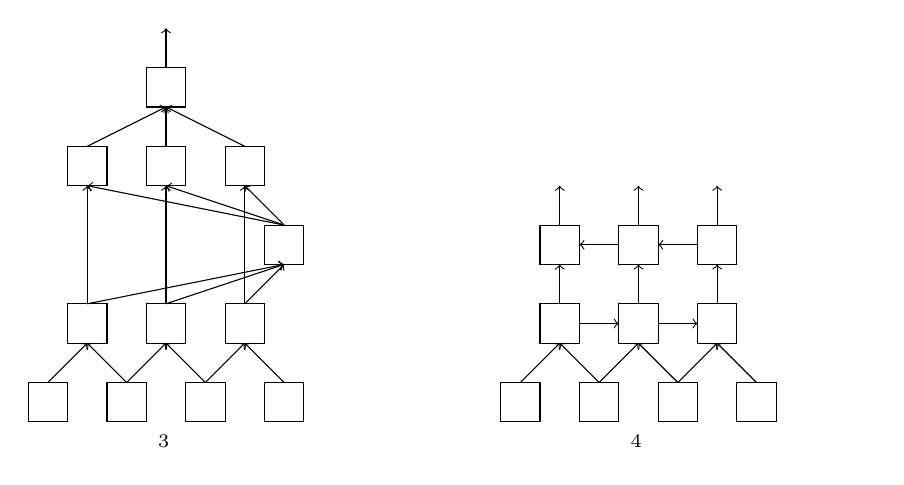
\begin{tikzpicture}
\foreach \i in {1,...,4}
{
	\draw (\i -7,0) rectangle (\i-7+0.5,0.5);
}
\foreach \i in {1,...,3}
{
	\draw (\i-7 + 0.5 ,1) rectangle (\i-7+1,1.5);
	\draw [->] (\i-7 +0.25  ,0.5) -- (\i-7 + 0.75 ,1);
	\draw [->] (\i-7 +1.25  ,0.5) -- (\i-7 + 0.75 ,1);
	\draw [->] (\i-7 + 0.75 ,1.5) -- (-2.75 ,2);
}
\draw (-3 ,2) rectangle (-2.5,2.5);
\foreach \i in {1,...,3}
{
	\draw (\i-7 + 0.5 ,3) rectangle (\i-7+1,3.5);
	\draw [->] (\i-7 +0.75, 1.5) -- (\i-7 +0.75,3);
	\draw [->] (-2.75, 2.5) -- (\i-7 +0.75,3);
	\draw [->] (\i-7 + 0.75 ,3.5) -- (-4.25 ,4);
}
\draw (-4.5 ,4) rectangle (-4,4.5);
\draw [->] (-4.25 ,4.5) -- (-4.25 ,5);
\node[text width=3cm] at (-2.85,-0.25) {$\cs_3$};
\foreach \i in {1,...,4}
{
	\draw (\i -1,0) rectangle (\i-1+0.5,0.5);
}
\foreach \i in {1,...,3}
{
	\draw (\i-1 + 0.5 ,1) rectangle (\i-1+1,1.5);
	\draw [->] (\i-1 +0.25  ,0.5) -- (\i-1 + 0.75 ,1);
	\draw [->] (\i-1 +1.25  ,0.5) -- (\i-1 + 0.75 ,1);
	\draw [->] (\i-1 + 0.75 ,1.5) -- (\i-1 + 0.75 ,2);
}
\draw [->] (1 ,1.25) -- (1.5 ,1.25);
\draw [->] (2 ,1.25) -- (2.5 ,1.25);
\foreach \i in {1,...,3}
{
	\draw (\i-1 + 0.5 ,2) rectangle (\i-1+1,2.5);
	\draw [->] (\i-1 + 0.75 ,2.5) -- (\i-1 + 0.75 ,3);
}
\draw [->] (1.5 ,2.25) -- (1 ,2.25);
\draw [->] (2.5 ,2.25) -- (2 ,2.25);
\node[text width=3cm] at (3.15,-0.25) {$\cs_4$};
\end{tikzpicture}
\caption{Examples of computation skeletons.\label{fig:cs_examples}}
\end{center}
\end{figure}

Figure \ref{fig:cs_examples} shows four example skeletons, omitting
the designation of the activation functions. The skeleton
$\cs_1$ is rather basic as it aggregates all the inputs in a single
step. Such topology can be useful in the absence of any prior
knowledge of how the output label may be computed from an input example, and
it is commonly used in natural language processing where the input is
represented as a bag-of-words~\cite{harris1954distributional}. The only structure in $\cs_1$
is a single {\em fully connected} layer:
\begin{terminology}[Fully connected layer of a skeleton]
%
An induced subgraph of a skeleton with $r+1$ nodes, $u_1,\ldots,u_r,v$, is
called a {\em fully connected layer} if its edges are
$u_1v,\ldots,u_rv$.
%
\end{terminology}
The skeleton $\cs_2$ is slightly more involved: it first processes
consecutive (overlapping) parts of the input, and the next layer
aggregates the partial results. Altogether, it corresponds to networks
with a single one-dimensional convolutional layer, followed by a fully
connected layer. The two-dimensional (and deeper) counterparts of such skeletons
correspond to networks that are common in visual object recognition.
\begin{terminology}[Convolution layer of a skeleton]
%
Let $s,w,q$ be positive integers and denote $n=s(q-1)+w$. A subgraph
of a skeleton is a one dimensional {\em convolution layer} of width $w$ and stride $s$
if it has $n+q$ nodes, $u_1,\ldots,u_{n}, v_1,\ldots,v_q$, and $q w$ edges,
$u_{s(i-1)+j}\,v_{i}$, for $1\le i\le q,1\le j\le w$.
%
\end{terminology}
%% The skeleton $\cs_3$ is a somewhat more sophisticated version of $\cs_2$, in
%% which after the local computations, a global computation is carried out
%% through a single aggregation node. The local computations are then
%% reassessed and finally aggregated again. The last skeleton, $\cs_4$, can be
%% useful for learning sequence-to-sequence mappings and similar skeletons
%% often used in translation, speech recognition, and OCR tasks.
The skeleton $\cs_3$ is a somewhat more sophisticated version of $\cs_2$: the local computations are first aggregated, then reconsidered with the aggregate, and finally aggregated again.
%
The last skeleton, $\cs_4$, corresponds to the networks that arise in
learning sequence-to-sequence mappings as used in translation, speech
recognition, and OCR tasks (see for example~\citet{sutskever2014sequence}).

\subsection{From computation skeletons to neural networks}
%
%% We are now ready to describe how a skeleton when accompanied with a
The following definition shows how a skeleton, accompanied with a
replication parameter $r\ge 1$ and a number of output nodes $k$,
induces a neural network architecture. Recall that inputs are ordered
sets of vectors in $\sphere^{d-1}$.
%% For brevity, we omit $d$ from the
%% notation introduced in the following definition.
%
\begin{definition}[Realization of a skeleton]
%
Let $\cs$ be a computation skeleton and consider input coordinates in
$\sphere^{d-1}$ as in \eqref{eq:coordinates}. For $r, k \ge 1$ we
define the following neural network $\cn=\cn(\cs,r,k)$.
%
For each input node in $\cs$, $\cn$ has $d$ corresponding input
neurons with weight $1/d$. For each internal node $v\in \cs$ labeled by an activation
$\sigma$, $\cn$ has $r$ neurons $v^1,\ldots,v^r$, each with an
activation $\sigma$ and weight $1/r$. In addition, $\cn$ has $k$ output neurons
$o_1,\ldots,o_k$ with the identity activation $\sigma(x)=x$ and weight $1$.
%
There is an edge $v^iu^j\in E(\cn)$ whenever $uv\in
E(\cs)$.  For every output node $v$ in $\cs$, each neuron $v^j$ is
connected to all output neurons $o_1,\ldots,o_k$. We term $\cn$ the
{\em $(r,k)$-fold realization} of $\cs$. We also define the {\em $r$-fold realization} of $\cs$ as\footnote{Note that for every $k$,
$\netrep\left(\cn(\cs,r,1)\right)=\netrep\left(\cn(\cs,r,k)\right)$.} $\cn(\cs,r)= \netrep\left(\cn(\cs,r,1)\right)$.
%
\end{definition}

%
\noindent
Note that the notion of the replication parameter $r$ corresponds, in
the terminology of convolutional networks, to the number of
channels taken in a convolutional layer and to the number of hidden units
taken in a fully-connected layer.
%% We would like to note that the architectures obtained by realizations of
%% skeletons include naturally many of the standard architectures employed in
%% practice such as fully connected layers, in which $r$ corresponds to the
%% number of hidden neurons, and convolutional layers, in which $r$ corresponds
%% to the number of channels.

Figure~\ref{fig:ct_to_nn} illustrates a $(5,4)$- and $5$-realizations
of a skeleton with coordinate dimension $d=2$.  The
$(5,4)$-realization is a network with a single (one dimensional)
convolutional layer having $5$ channels, stride of $2$, and width of
$4$, followed by three fully-connected layers. The global replication
parameter $r$ in a realization is used for brevity; it is
straightforward to extend results when the different nodes in $\cs$
are each replicated to a different extent.

%% We would also like to note that
%% for brevity, we use same replication parameter $r$ for all nodes. It is
%% straightforward to extend the definition and the results presented
%% henceforth to the case when different nodes in $\cs$ are associated with
%% different replication values.

\begin{figure}[t]
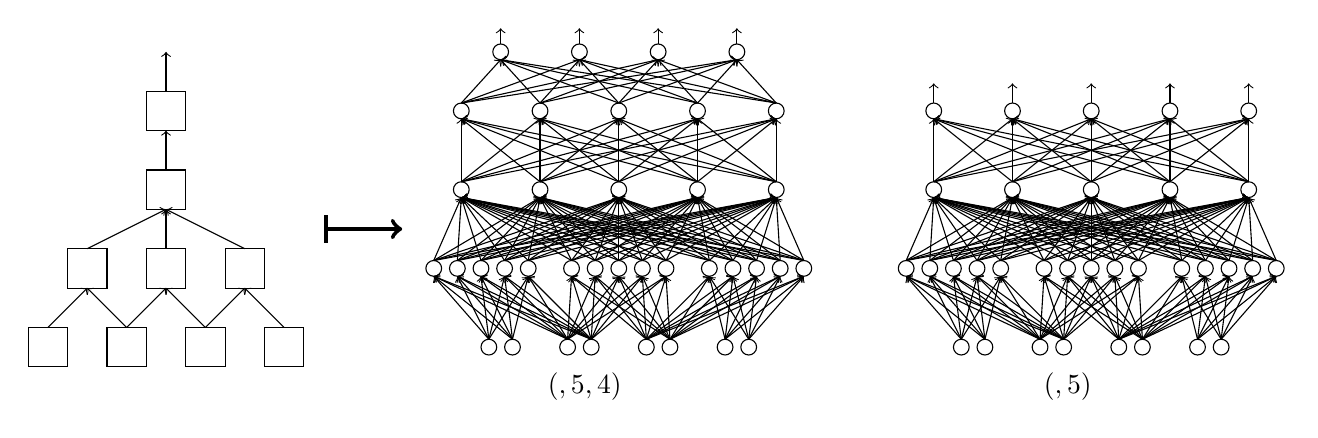
\begin{tikzpicture}
\foreach \i in {1,...,4}
{
	\draw (\i -1,0) rectangle (\i-1+0.5,0.5);
}
\foreach \i in {1,...,3}
{
	\draw (\i-1 + 0.5 ,1) rectangle (\i-1+1,1.5);
	\draw [->] (\i-1 +0.25  ,0.5) -- (\i-1 + 0.75 ,1);
	\draw [->] (\i-1 +1.25  ,0.5) -- (\i-1 + 0.75 ,1);
	\draw [->] (\i-1 + 0.75 ,1.5) -- (1.75 ,2);
}
\draw (1.5 ,2) rectangle (2,2.5);
\draw [->] (1.75 ,2.5) -- (1.75 ,3);
\draw (1.5 ,3) rectangle (2,3.5);
\draw [->] (1.75 ,3.5) -- (1.75 ,4);
\node[text width=3cm] at (3.15,-0.25) {$\cs$};
\draw [ultra thick, |->] (3.75,1.75) -- (4.75,1.75);
\foreach \i in {1,...,4}
{
	\draw (4.85+\i,0.25) circle [radius=0.1];
	\draw (5.15+\i,0.25) circle [radius=0.1];
}
\foreach \i in {-1,...,1}
{
	\foreach \j in {-2,...,2}
	{
		\draw (7.5+1.75*\i + 0.3*\j,1.25) circle [radius=0.1];
		\draw [->] (6.85+\i,0.35) -- (7.5+1.75*\i + 0.3*\j,1.15);
		\draw [->] (7.15+\i,0.35) -- (7.5+1.75*\i + 0.3*\j,1.15);

		\draw [->] (7.85+\i,0.35) -- (7.5+1.75*\i + 0.3*\j,1.15);
		\draw [->] (8.15+\i,0.35) -- (7.5+1.75*\i + 0.3*\j,1.15);
		\foreach \k in {-2,...,2}
		{
			\draw [->] (7.5+1.75*\i + 0.3*\j,1.35) -- (7.5+\k,2.15);
		}
	}
}
\foreach \j in {-2,...,2}
{
	\draw (7.5+\j,2.25) circle [radius=0.1];
	\foreach \k in {-2,...,2}
	{
		\draw[->] (7.5+\j,2.35) -- (7.5+\k,3.15);
	}
}
\foreach \j in {-2,...,2}
{
	\draw (7.5+\j,3.25) circle [radius=0.1];
	\draw[->] (7.5+\j,3.35) -- (6,3.9);
	\draw[->] (7.5+\j,3.35) -- (7,3.9);
	\draw[->] (7.5+\j,3.35) -- (8,3.9);
	\draw[->] (7.5+\j,3.35) -- (9,3.9);
}
\draw (6,4) circle [radius=0.1];
\draw (7,4) circle [radius=0.1];
\draw (8,4) circle [radius=0.1];
\draw (9,4) circle [radius=0.1];
\draw[->] (6,4.1) -- (6,4.3);
\draw[->] (7,4.1) -- (7,4.3);
\draw[->] (8,4.1) -- (8,4.3);
\draw[->] (9,4.1) -- (9,4.3);
\node[text width=3cm] at (8.1,-0.25) {$\cn(\cs,5,4)$};
\foreach \i in {1,...,4}
{
	\draw (10.85+\i,0.25) circle [radius=0.1];
	\draw (11.15+\i,0.25) circle [radius=0.1];
}
\foreach \i in {-1,...,1}
{
	\foreach \j in {-2,...,2}
	{
		\draw (6+7.5+1.75*\i + 0.3*\j,1.25) circle [radius=0.1];
		\draw [->] (6+6.85+\i,0.35) -- (6+7.5+1.75*\i + 0.3*\j,1.15);
		\draw [->] (6+7.15+\i,0.35) -- (6+7.5+1.75*\i + 0.3*\j,1.15);

		\draw [->] (6+7.85+\i,0.35) -- (6+7.5+1.75*\i + 0.3*\j,1.15);
		\draw [->] (6+8.15+\i,0.35) -- (6+7.5+1.75*\i + 0.3*\j,1.15);
		\foreach \k in {-2,...,2}
		{
			\draw [->] (6+7.5+1.75*\i + 0.3*\j,1.35) -- (6+7.5+\k,2.15);
		}
	}
}
\foreach \j in {-2,...,2}
{
	\draw (6+7.5+\j,2.25) circle [radius=0.1];
	\foreach \k in {-2,...,2}
	{
		\draw[->] (6+7.5+\j,2.35) -- (6+7.5+\k,3.15);
	}
}
\foreach \j in {-2,...,2}
{
	\draw (6+7.5+\j,3.25) circle [radius=0.1];
	\draw[->] (6+7.5+\j,3.35) -- (6+7.5+\j,3.6);
}
\node[text width=3cm] at (6+8.4,-0.25) {$\cn(\cs,5)$};
\end{tikzpicture}
\caption{A $(5,4)$-fold and $5$-fold realizations of the computation
skeleton $\cs$ with $d=2$.\label{fig:ct_to_nn}}
\end{figure}

We next define a scheme for random initialization of the weights of a neural
network, that is similar to what is often done in practice. We employ the definition throughout the paper whenever we refer to
random weights.
%
\begin{definition}[Random weights]\label{def:rand_weights}
%
A {\em random initialization} of a neural network $\cn$ is a
multivariate Gaussian $\w=(w_{uv})_{uv\in E(\cn)}$ such that each weight
$w_{uv}$ is sampled independently from a normal distribution with mean $0$
and variance\footnote{For $U\subset V(\cn)$ we denote $\delta(U) = \sum_{u\in U}\delta(u)$.} ${d\delta(u)}/{\delta(\IN(v))}$ if $u$ is an input neuron and ${\delta(u)}/{\left(\|\sigma_{u}\|^2\,\delta(\IN(v))\right)}$ otherwise.
%
\end{definition}
%
%% In practice, weights are often sampled independently from
%% normal distributions with variance proportional to ${1}/{|\IN(v)|}$.
%% We would like to note that in many architectures, such as convolutional nets,
\noindent
Architectures such as convolutional nets have weights that are shared
across different edges.
% (i.e.\ the same weight is associated with different edges)
Again, it is straightforward to extend our results to these cases and for
simplicity we assume no explicit weight sharing.

\subsection{From computation skeletons to reproducing kernels}
%
In addition to networks' architectures, a computation skeleton $\cs$ also
defines a normalized kernel $\kappa_\cs:\cx\times\cx\to[-1,1]$ and a
corresponding norm $\|\cdot \|_{\cs}$ on functions $f:\cx\to\reals$. This
norm has the property that $\|f\|_{\cs}$ is small if and only if $f$ can be
obtained by certain simple compositions of functions according to the
structure of $\cs$. To define the kernel,
we introduce a {\em dual activation} and {\em dual kernel}. For
$\rho\in[-1,1]$, we denote by $\gaussian_\rho$ the multivariate Gaussian
distribution on $\reals^2$ with mean $0$ and covariance matrix
$\left( \begin{smallmatrix} 1 & \rho \\ \rho & 1 \end{smallmatrix} \right)$.
%% whose diagonal elements are $1$ and off-diagonal elements are $\rho$.
%% \iffalse
%% $\begin{pmatrix} 1 & \rho \\ \rho & 1 \end{pmatrix}$.
%% \fi
%

\begin{definition}[Dual activation and kernel]\label{def:dual_act}
%
The {\em dual activation} of an activation $\sigma$ is the function
$\hat{\sigma}:[-1,1]\to\reals$ defined as
$$
\hat\sigma(\rho) =
	\E_{(X,Y) \sim \gaussian_\rho}\sigma(X)\sigma(Y) \,.
$$
The {\em dual kernel} w.r.t.\ to a Hilbert space $\ch$ is the kernel
$\kappa_\sigma:\ch^1\times \ch^1\to\reals$ defined as
$$\kappa_\sigma(\x,\y) = \hat{\sigma}(\inner{\x,\y}_\ch) \,.$$

%
\end{definition}
%
\noindent
Section~\ref{sec:comp_ker} shows that $\kappa_\sigma$ is indeed a kernel for every activation
$\sigma$ that adheres with the square-integrability requirement.
%
In fact,
any continuous $\mu:[-1,1]\to\reals$, such that
$(\x,\y)\mapsto\mu(\inner{\x,\y}_\ch)$ is a kernel for all $\ch$, is
the dual of some activation.
%
Note that $\kappa_\sigma$ is normalized iff $\sigma$ is normalized.
%
We show in Section~\ref{dualact:sec} that dual activations are closely
related to Hermite polynomial expansions, and that these can be used
to calculate the duals of activation functions analytically.
%
Table~\ref{tab:duals} lists a few examples of normalized activations
and their corresponding dual (corresponding derivations are in
Section~\ref{dualact:sec}).
%
{\renewcommand{\arraystretch}{1.3}%
\begin{table}[t]
\begin{center}
  \begin{tabular}{lllll}
    \hline
    Activation &  & Dual Activation & Kernel & Ref \\ \hline
    Identity & $x$ & $\rho$ & linear\\
    2nd Hermite & $\frac{x^2 - 1}{\sqrt{2}}$ & $\rho^2$ & poly &\\
    ReLU & $\sqrt{2}\,[x]_+$ &
		$\frac{1}{\pi}+\frac{\rho}{2} +
		 \frac{\rho^2}{2\pi} +
		 \frac{\rho^4}{24\pi} + \ldots
		 = \frac{\sqrt{1-\rho^2}+(\pi-\cos^{-1}(\rho))\rho}{\pi}$ &
		 $\arccos_1$  & \cite{cho2009kernel}\\
    Step & $\sqrt{2}\,\ind[{x\ge 0}]$ &
			$\frac{1}{2} +
			 \frac{\rho}{\pi} +
			 \frac{\rho^3}{6\pi} +
			 \frac{3\rho^5}{40\pi} + \ldots = \frac{\pi-\cos^{-1}(\rho)}{\pi}$ &
			 $\arccos_0$ & \cite{cho2009kernel}\\
    Exponential & $e^{x-2}$ &
			$\frac{1}{e}+\frac{\rho}{e}+\frac{\rho^2}{2e}+\frac{\rho^3}{6e}+\ldots=
			e^{\rho-1}$ & RBF & \cite{mairal2014convolutional}\\
			& & & & \vspace{-16pt} \\
			\hline
  \end{tabular}
\caption{Activation functions and their duals.\label{tab:duals}}
\end{center}
\end{table}
}
%
The following definition gives the kernel corresponding to a skeleton
having normalized activations.\footnote{For a skeleton $\cs$ with unnormalized
  activations, the corresponding kernel is the kernel of the skeleton
  $\cs'$ obtained by normalizing the activations of $\cs$.}
%
\begin{definition}[Compositional kernels]\label{def:comp_ker}
%
Let $\cs$ be a computation skeleton with normalized activations and
(single) output node $o$.
%
For every node $v$, inductively define a kernel
$\kappa_v:\cx\times\cx\to\reals$ as follows.
%
For an input node $v$ corresponding to the $i$th coordinate,
define $\kappa_{v}(\x,\y)=\inner{\x^i, \y^i}$.
%
For a non-input node $v$, define
$$
\kappa_v(\x,\y) =
	\hat\sigma_v\left(
		\frac{\sum_{u\in \IN(v)}\kappa_{u}(\x,\y)}{|\IN(v)|}\right) \,.
    $$
The final kernel $\kappa_\cs$ is $\kappa_o$, the kernel associated with
the output node $o$. The resulting Hilbert space and norm are
denoted $\ch_\cs$ and $\|\cdot\|_\cs$ respectively, and
$\ch_v$ and $\|\cdot\|_v$ denote the space and norm when formed at node $v$.
\end{definition}
%
\noindent As we show later, $\kappa_\cs$ is indeed a (normalized) kernel for every
skeleton $\cs$. To understand the kernel in the context of learning, we need
to examine which functions can be expressed as moderate
norm functions in $\ch_\cs$. As we show in section \ref{sec:comp_ker},
these are the functions obtained by certain simple compositions according to the
feed-forward structure of $\cs$. For intuition, the following example
contrasts two commonly used skeletons.

\begin{example}[Convolutional vs.\ fully connected skeletons]
\label{exam:diff_struct}
Consider a network whose activations are all ReLU, $\sigma(z)=[z]_+$,
and an input space $\cx_{n,1}=\{\pm 1\}^n$. Say that $\cs_1$ is a
skeleton comprising a single fully connected layer, and that $\cs_2$ is one comprising
a convolutional layer of stride $1$ and width $q=\log^{0.999}(n)$, followed by a single fully-connected layer. (The skeleton $\cs_2$ from
Figure~\ref{fig:cs_examples} is a concrete example of the convolutional
skeleton with $q=2$ and $n=4$.)
%
The kernel $\kappa_{\cs_1}$ takes the form $\kappa_{\cs_1}(\x,\y) =
\hat{\sigma} \left({\inner{\x,\y}}/{n}\right)$. It is a symmetric kernel and
therefore functions with small norm in $\ch_{\cs_1}$ are essentially
low-degree polynomials. For instance, fix a bound $R=n^{1.001}$ on the norm
of the functions.
In this case, the space $\ch^{R}_{\cs_1}$ contains
multiplication of one or two input coordinates. However, multiplication of
$3$ or more coordinates are no-longer in $\ch^{R}_{\cs_1}$. Moreover, this
property holds true regardless of the choice of activation
function. On the other hand, $\ch^{R}_{\cs_2}$ contains functions
whose dependence on adjacent input coordinates is far more complex. It includes,
for instance, any function $f:\cx\to \{\pm 1\}$ that is symmetric
(i.e.\ $f(x)=f(-x)$) and that depends on $q$ adjacent coordinates
$\x_{i},\ldots,\x_{i+q}$. Furthermore, any sum of $n$ such functions is
also in $\ch^{R}_{\cs_2}$.
\end{example}

\section{Empirical Evaluation}
We trained a series of models of various sizes. For all subsequent evaluations, we will use the largest model (referred to as CogVideoX).
In this section, we present the experimental validation of CogVideoX through two primary methods: automated metric evaluation and human assessment, providing a thorough analysis of the performance and quality of the generated videos. 
We trained a series of models with different parameter sizes. The following evaluation defaults to using our largest model.

\subsection{Results of Automated Metric Evaluation} 

\paragraph{Baselines.} We chose several top-performing text-to-video models as our baselines for comparison, including T2V-Turbo~\citep{li2024t2v}, AnimateDiff~\citep{guo2023animatediff}, VideoCrafter2~\citep{chen2024videocrafter2}, OpenSora~\citep{opensora}, Show-1~\citep{zhang2023show}, Gen-2~\citep{gen2}, Pika~\citep{pika} and LaVie-2~\citep{wang2023lavie}.


% \begin{figure}[h]
% \begin{center}
% \includegraphics[width=0.9\linewidth]{images/bench_eval.png}
% \end{center}
% \caption{The radar chart comparing the performance of different models.}
% \label{fig:radar}
% \end{figure}

\hide{
%\begin{wrapfigure}{r}{0.5\textwidth}
\begin{figure}
\centering
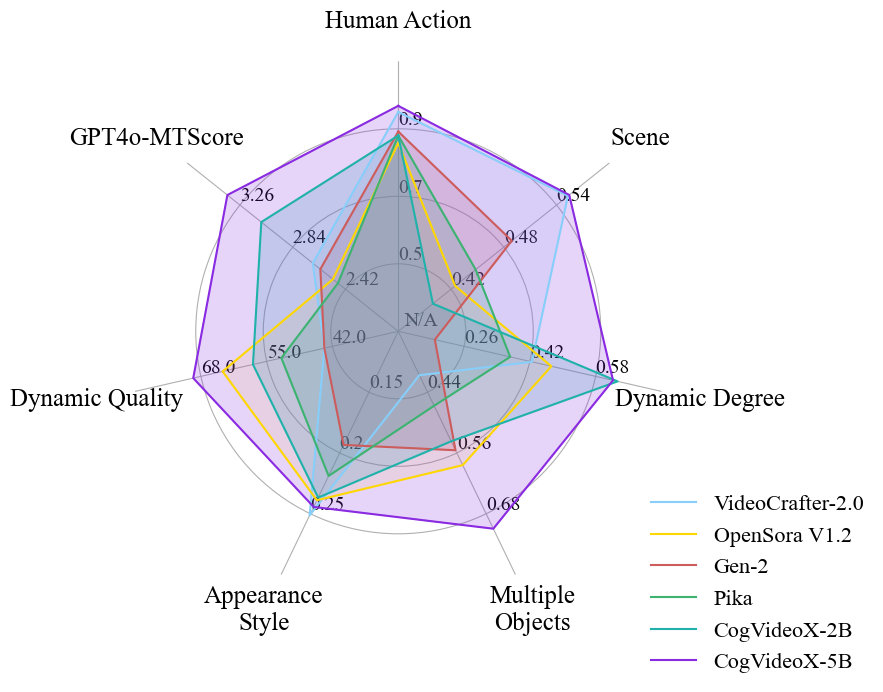
\includegraphics[width=0.7\linewidth]{images/bench_eval9.png}
\caption{The radar chart comparing the performance of different models. CogVideoX represents the largest one. It is clear that CogVideoX outperforms its competitors in the vast majority of metrics, and it is very close to the leading models in the remaining indicator.
}
\label{fig:radar}
% \vspace{-10mm}
%\end{wrapfigure}

\end{figure}

}%end ofhide
\paragraph{Evaluation Metrics.} To evaluate the text-to-video generation, we employed several metrics from VBench~\citep{huang2023vbench}: \emph{Human Action}, \emph{Scene}, \emph{Dynamic Degree}, \emph{Multiple Objects}, and \emph{Appearance Style}. VBench is a suite of tools designed to automatically assess the quality of generated videos. We have selected certain metrics from VBench, excluding others that do not align with our evaluation needs. For example, the color metric, intended to measure the presence of objects corresponding to specific colors across frames in the generated video, assesses the model's quality by calculating the probability. However, this metric may mislead video generation models that exhibit greater variation, thus we chose not to include it in our evaluation. For longer-generated videos, some models might produce videos with minimal changes between frames to obtain higher scores, but these videos lack rich content. Therefore, a metric for evaluating the dynamism of the video becomes more important. To address this, we employed two video evaluation tools, We also employed the \emph{Dynamic Quality} from Devil~\citep{liao2024evaluationtexttovideogenerationmodels} and \emph{GPT4o-MTScore} from ChronoMagic~\citep{yuan2024chronomagic}, which focus more on the dynamic characteristics of videos. \emph{Dynamic Quality} is defined by the integration of various quality metrics with dynamic scores. This approach mitigates biases arising from negative correlations between video dynamics and video quality, leading to a more thorough assessment of video quality. ChronoMagic, for instance, introduces the \emph{GPT4o-MTScore}, a metric designed to measure the metamorphic amplitude of time-lapse videos, such as those depicting physical, biological, and meteorological changes. This metric is obtained by extracting frames from the generated videos at regular intervals and using GPT-4o~\citep{gpt4o} to score the degree of change, providing a fine-grained assessment of video dynamism. This method ensures a more accurate evaluation of the content's variability over time, countering the potential bias of static frame sequences in scoring.



\paragraph{Results.} Table~\ref{table:results} provides a detailed comparison of the performance of our CogVideoX model with other models. Our model achieved the best performance in 5 out of the 7 metrics and showed competitive results in the remaining 2 metrics. These results demonstrate that our model not only excels in video generation quality but also outperforms previous models in handling various complex dynamic scenes. Additionally, Figure~\ref{fig:radar} presents a radar chart comparing the performance of different models.


\begin{figure}[ht]
\begin{center}
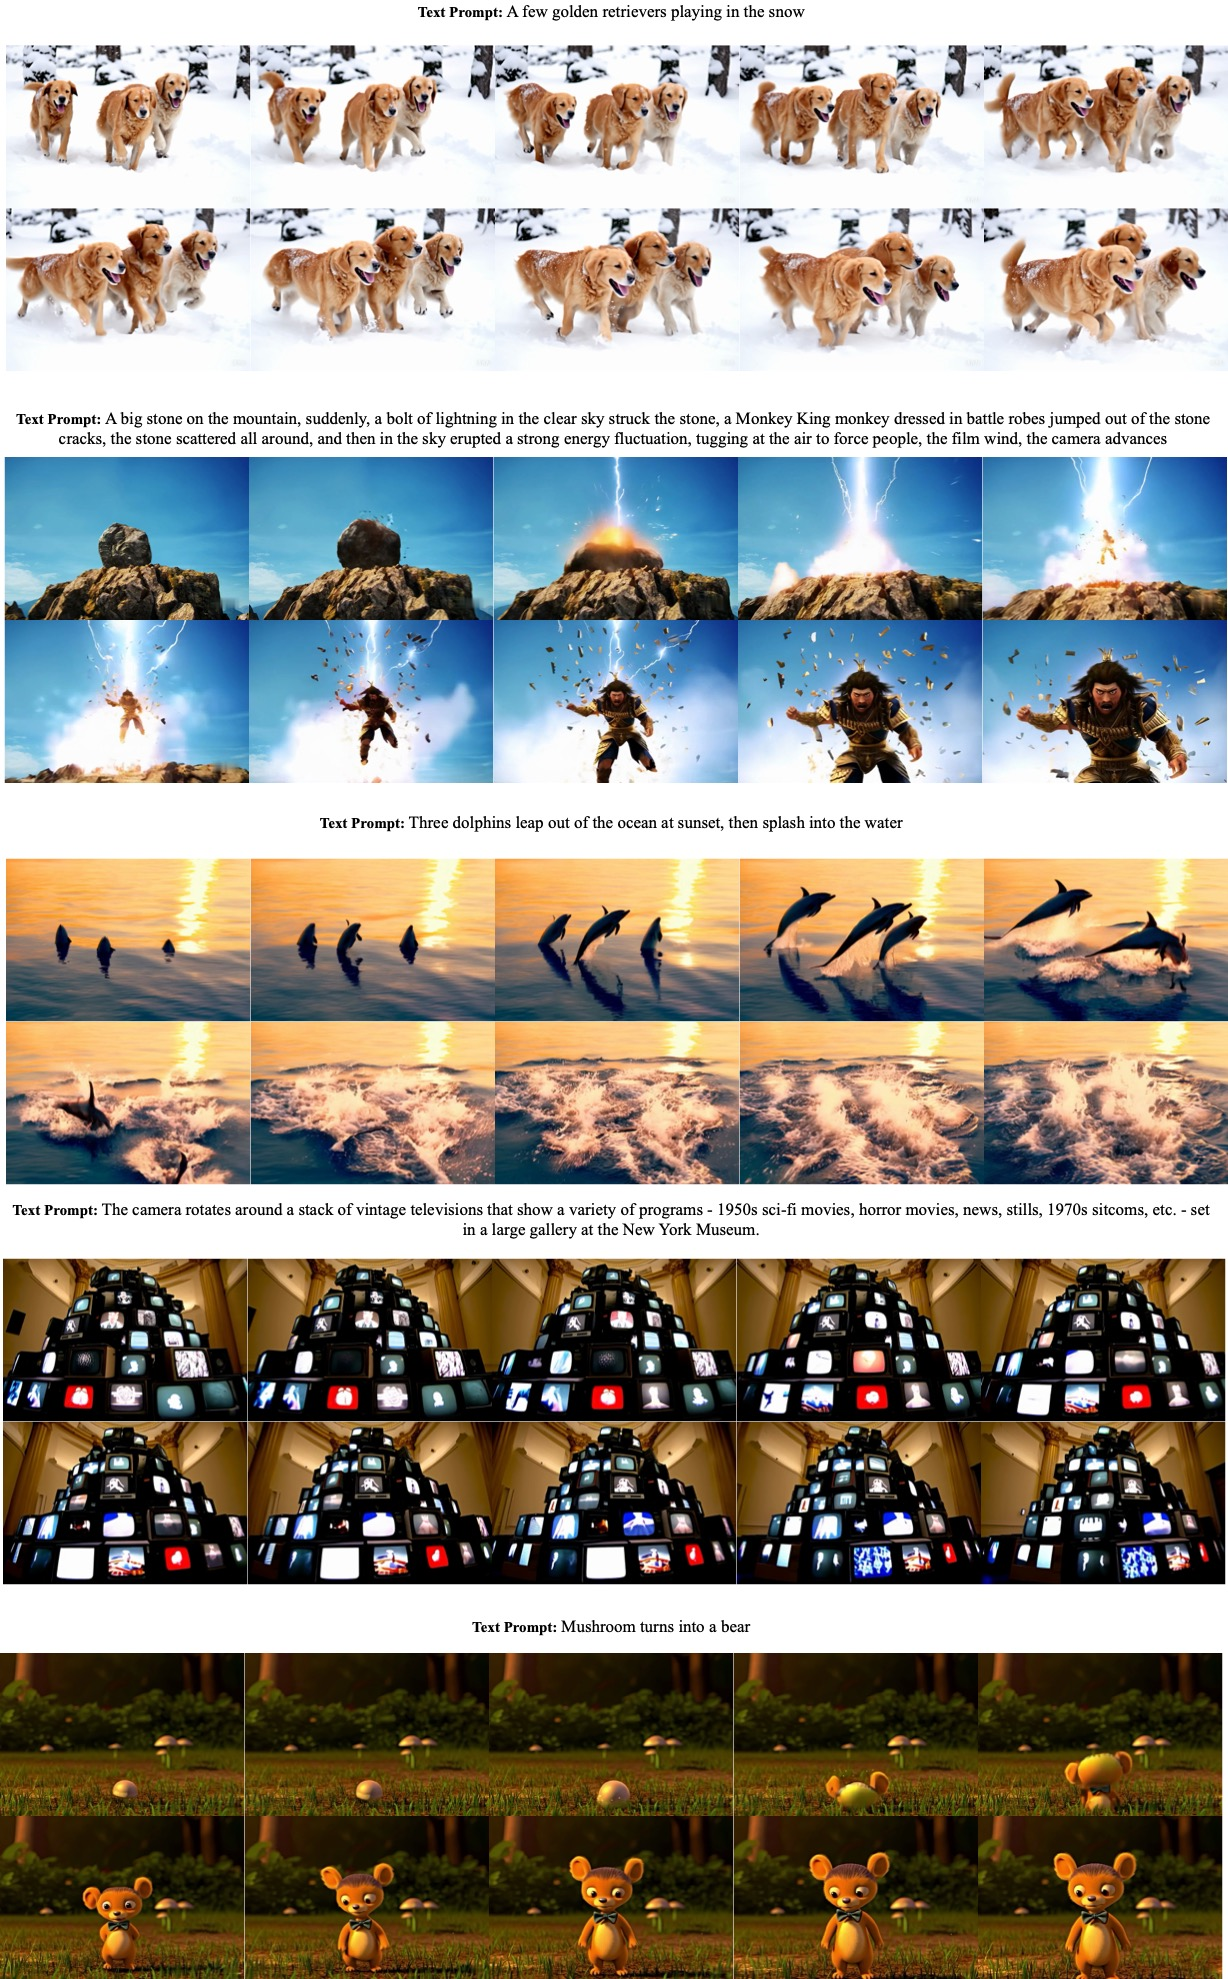
\includegraphics[width=\linewidth]{images/t2v/goodcase1.jpg}
\end{center}
\caption{Text to video showcases. The displayed prompt will be upsampled before being fed into the model. The generated videos contain large motion and can produce various video styles.}
\label{fig:t2vgood1}
\end{figure}

\begin{figure}[ht]
\begin{center}
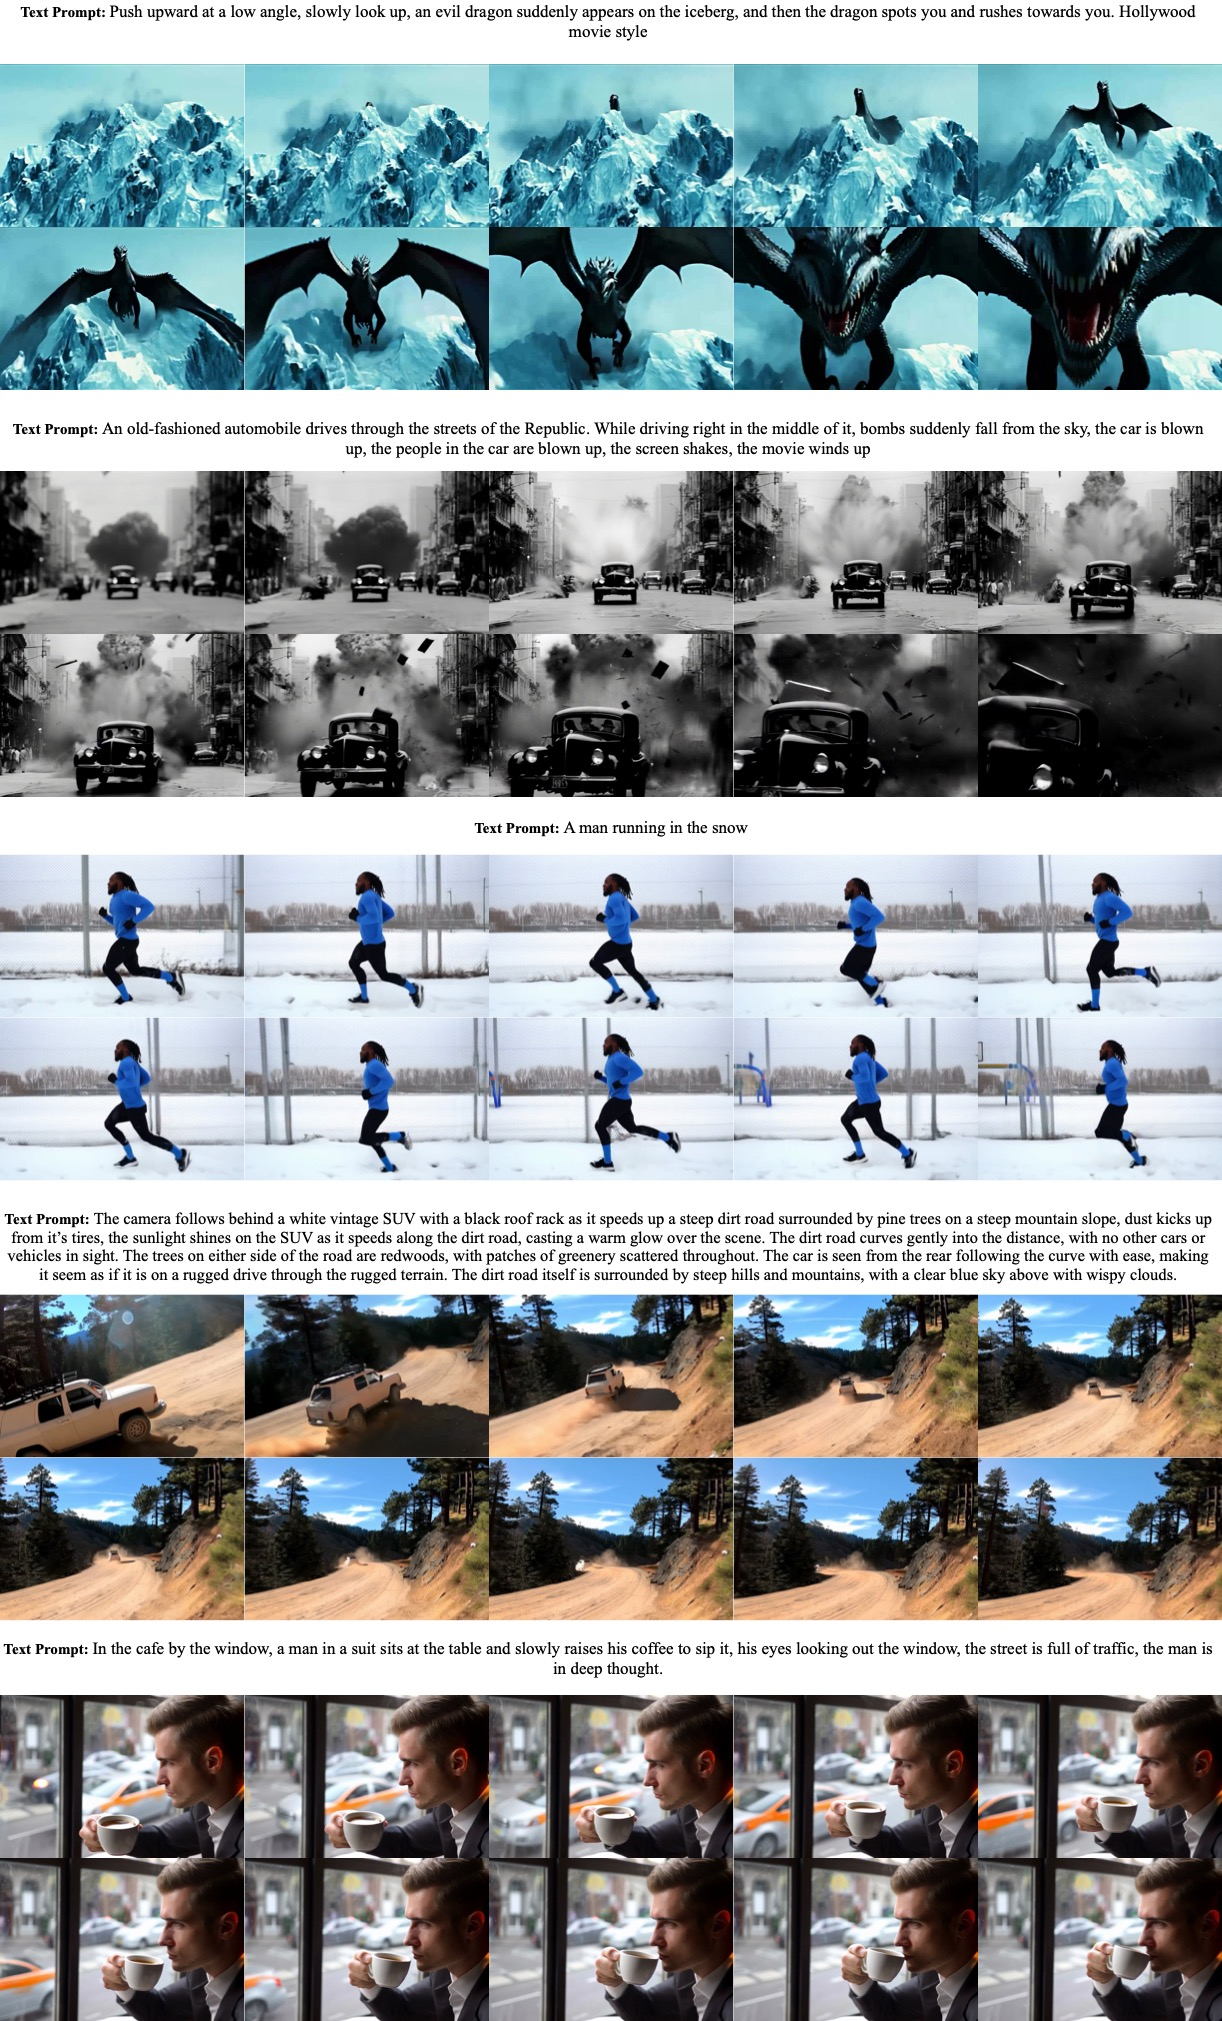
\includegraphics[width=0.98\linewidth]{images/t2v/goodcase2.jpg}
\end{center}
\caption{Text to video showcases.}
\label{fig:t2vgood2}
\end{figure}


% Please add the following required packages to your document preamble:
% \usepackage[table,xcdraw]{xcolor}
% Beamer presentation requires \usepackage{colortbl} instead of \usepackage[table,xcdraw]{xcolor}
% \usepackage[normalem]{ulem}
% \useunder{\uline}{\ul}{}




% \begin{table}[]

% \centering
% \setlength\tabcolsep{3pt}

% \label{sample-table}
% \small
% \vspace{-10pt}
% \caption{\textbf{Automatic Evaluation Results per Dimension.}The table presents a comparative analysis of various video models across different dimensions. It is evident from the table that, in terms of both human motion and background effects as well as the accuracy and distinctiveness of objects, CogVideoX has achieved the current SOTA level. Furthermore, CogVideoX has garnered a commendable score in the expression of dynamic qualities, a capability that serves as a more precise indicator of the intrinsic properties of video media, distinct from the static nature of photographic images.}

% \vspace{6pt}

% \begin{tabular}{cccccccc}
% \toprule
% \multirow{2}{*}{\textbf{Models} }  & \textbf{human}  & \textbf{object} &\multirow{2}{*}{\textbf{scene}}&\textbf{dynamic} &\textbf{multiple} &\textbf{spatial} &\textbf{appearance} \\
%     & \textbf{action}& \textbf{class}& & \textbf{degree} &\textbf{objects}& \textbf{relationship}&\textbf{style}  
% \\
% \midrule
% CogVideoX & 96.80\% &93.70\% & 55.44\% & 62.22\% & 70.95\% & 61.29\% & 24.44\% \\
% {LaVie-2} & 96.40\% & 97.52\%  & 49.59\% & 31.11\% & 64.88\%  & 38.68\% & 25.09\%  \\
% {T2V-Turbo}  & 95.20\%  & 93.96\%& 55.58\% & 49.17\% & 54.65\%    & 38.67\%  & 24.42\%   \\
% {Gen-2}  & 89.20\%& 90.92\%  & 48.91\%  & 18.89\% & 55.47\%    & 66.91\%   & 19.34\%  \\
% {VideoCrafter-2.0\citep{chen2024videocrafter2}} & 95.00\% & 92.55\% & 55.29\%               & 42.50\% & 40.66\% & 35.86\% & 25.13\%  \\
% {Pika Beta} & 88.00\% & 87.45\%  & 44.80\% & 37.22\% & 46.69\% & 65.65\% & 21.89\%   \\
% AnimateDiff-V2 & 92.60\% & 90.90\%  & 50.19\% & 40.83\%        & 36.88\% & 34.60\%  & 22.42\%\\
% {OpenSora V1.2}   & 85.80\% & 83.37\%& 42.47\%   & 47.22\%    & 58.41\% & 67.51\%  & 23.89\%  \\
% {Show-1} & 95.60\%  & 93.07\%  & 47.03\% & 44.44\% & 45.47\% & 53.50\%  & 23.06\%  \\
% {HiGen}  & 86.20\%  & 86.06\%  & 44.88\% & 99.17\% & 22.39\%  & 22.43\% & 24.54\% \\  
% \bottomrule
% \end{tabular}
% \end{table}



% \iffalse



% \begin{table}[ht!]
% \centering
% \caption{Evaluation results.}
% \setlength\tabcolsep{3pt}
% \label{sample-table}
% \begin{center}
% \small
% \resizebox{0.9\linewidth}{!}{
% \begin{tabular}{ccccccccc}

% \multirow{2}{*}{\textbf{Models} }  & \textbf{subject}  & \textbf{background} &\textbf{temporal} &\textbf{motion} &\textbf{dynamic} &\textbf{aesthetic} &\textbf{imaging} &\textbf{object} \\
%     & \textbf{consistency}& \textbf{consistency}& \textbf{flickering}& \textbf{smoothness} &\textbf{degree}& \textbf{quality}&\textbf{quality} & \textbf{class}
% \\ \hline 
%         CogVideoX & 94.66\% & 95.92\% & 97.47\% & 98.10\% & 62.22\% & 55.14\% & 63.62\% & 93.70\%  \\
%         LaVie-2 & 97.90\% & 98.45\% & 98.76\% & 98.42\% & 31.11\% & 67.62\% & 70.39\% & 97.52\%  \\ 
%         T2V-Turbo (VC2) & 96.28\% & 97.02\% & 97.48\% & 97.34\% & 49.17\% & 63.04\% & 72.49\% & 93.96\%  \\ 
%         Gen-2 (2023-06) & 97.61\% & 97.61\% & 99.56\% & 99.58\% & 18.89\% & 66.96\% & 67.42\% & 90.92\%  \\ 
%         VideoCrafter-2.0\citep{chen2024videocrafter2} & 96.85\% & 98.22\% & 98.41\% & 97.73\% & 42.50\% & 63.13\% & 67.22\% & 92.55\%  \\ 
%         Pika Beta (2023-06) & 96.76\% & 98.95\% & 99.77\% & 99.51\% & 37.22\% & 63.15\% & 62.33\% & 87.45\%  \\ 
%         AnimateDiff-V2 & 95.30\% & 97.68\% & 98.75\% & 97.76\% & 40.83\% & 67.16\% & 70.10\% & 90.90\%  \\ 
%         OpenSora V1.2 & 94.45\% & 97.90\% & 99.47\% & 98.20\% & 47.22\% & 56.18\% & 60.94\% & 83.37\%  \\ 
%         Show-1 & 95.53\% & 98.02\% & 99.12\% & 98.24\% & 44.44\% & 57.35\% & 58.66\% & 93.07\%  \\ 
%         HiGen & 90.07\% & 93.99\% & 93.24\% & 96.69\% & 99.17\% & 57.30\% & 63.92\% & 86.06\% \\ 
% \hline \\

% \multirow{2}{*}{\textbf{Models} }  & \textbf{multiple}  & \textbf{human} &\multirow{2}{*}{\textbf{color}} &\textbf{spatial} &\multirow{2}{*}{\textbf{scene}} &\textbf{appearance} &\textbf{temporal} &\textbf{overall} \\
%     & \textbf{objects}& \textbf{action}& & \textbf{relation} & & \textbf{style}&\textbf{style} & \textbf{consistency}
% \\ \hline 
%         CogVideoX & 70.95\% & 96.80\% & 79.75\% & 61.29\% & 55.44\% & 24.44\% & 23.69\% & 26.73\%  \\ 
%         LaVie-2 & 64.88\% & 96.40\% & 91.65\% & 38.68\% & 49.59\% & 25.09\% & 25.24\% & 27.39\%  \\ 
%         T2V-Turbo (VC2) & 54.65\% & 95.20\% & 89.90\% & 38.67\% & 55.58\% & 24.42\% & 25.51\% & 28.16\%  \\
%         Gen-2 (2023-06) & 55.47\% & 89.20\% & 89.49\% & 66.91\% & 48.91\% & 19.34\% & 24.12\% & 26.17\%  \\ 
%         VideoCrafter-2.0 & 40.66\% & 95.00\% & 92.92\% & 35.86\% & 55.29\% & 25.13\% & 25.84\% & 28.23\%  \\
%         Pika Beta (2023-06) & 46.69\% & 88.00\% & 85.31\% & 65.65\% & 44.80\% & 21.89\% & 24.44\% & 25.47\%  \\ 
%         AnimateDiff-V2 & 36.88\% & 92.60\% & 87.47\% & 34.60\% & 50.19\% & 22.42\% & 26.03\% & 27.04\%  \\ 
%         OpenSora V1.2 & 58.41\% & 85.80\% & 87.49\% & 67.51\% & 42.47\% & 23.89\% & 24.55\% & 27.07\%  \\ 
%         Show-1 & 45.47\% & 95.60\% & 86.35\% & 53.50\% & 47.03\% & 23.06\% & 25.28\% & 27.46\%  \\ 
%         HiGen & 22.39\% & 86.20\% & 86.22\% & 22.43\% & 44.88\% & 24.54\% & 25.14\% & 27.14\% \\ \hline

% \hline \\
% \end{tabular}

% }
% \end{center}
% \end{table}

% \fi






% \begin{table}[!ht]
% \centering

% \label{sample-table}
% \small
% \vspace{-10pt}
% \caption{\textbf{Automatic Evaluation Results per Dimension.}}

% \vspace{6pt}

% \resizebox{0.8\linewidth}{!}{
%     \begin{tabular}{cccc}
%         \textbf{Models} & \textbf{\Centerstack{Dynamics Range}} & \textbf{\Centerstack{Dynamics Controllability}} & \textbf{\Centerstack{Dynamics-based Quality}} \\ \hline
%         CogVideoX       & 55.7 & 71.8 & \textbf{69.5} \\ 
%         Gen-2           & 30.8 & \textbf{82.5} & 43.6 \\ 
%         Pika            & 43.2 & 72.0 & 52.1 \\ 
%         VideoCrafter2   & 34.1 & 57.0 & 43.6 \\ 
%         OpenSora        & \textbf{61.2} & 62.4 & 63.7 \\ 
%         Show-1          & 45.1 & 73.9 & 57.7 \\ 
%     \end{tabular}
% }
% \end{table}


% \begin{figure}[h]
% \begin{center}
% \includegraphics[width=0.9\linewidth]{images/bench_eval.png}
% \end{center}
% \caption{The radar chart comparing the performance of different models.}
% \label{fig:radar}
% \end{figure}

\hide{
%\begin{wrapfigure}{r}{0.5\textwidth}
\begin{figure}
\centering
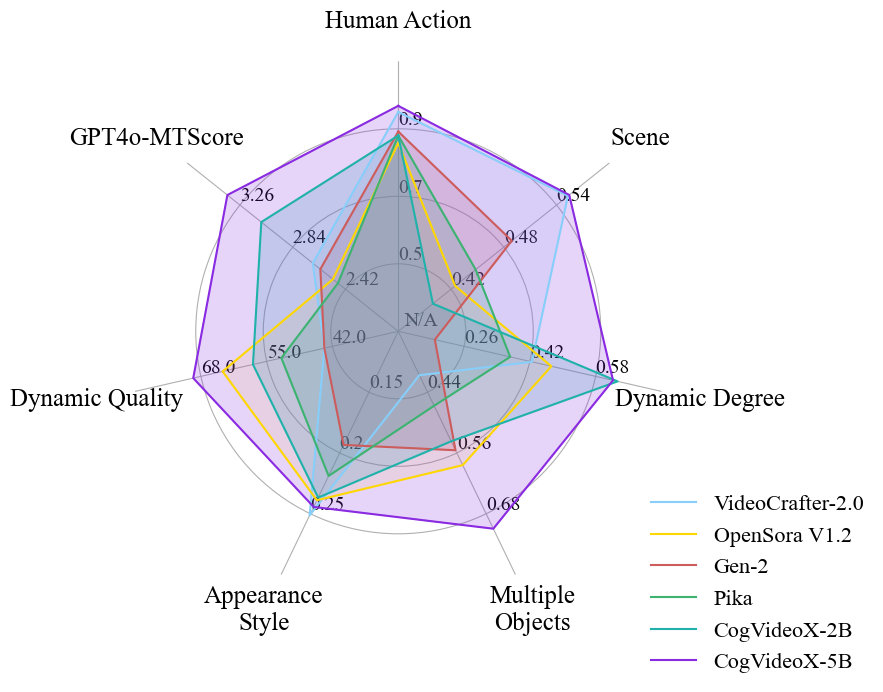
\includegraphics[width=0.7\linewidth]{images/bench_eval9.png}
\caption{The radar chart comparing the performance of different models. CogVideoX represents the largest one. It is clear that CogVideoX outperforms its competitors in the vast majority of metrics, and it is very close to the leading models in the remaining indicator.
}
\label{fig:radar}
% \vspace{-10mm}
%\end{wrapfigure}

\end{figure}

}%end ofhide


\subsection{Human Evaluation}
In addition to automated scoring mechanisms, a comparative analysis between the Kling~\citep{kling} and CogVideoX was conducted using a manual scoring system. One hundred meticulously crafted prompts were used, characterized by their broad distribution, clear articulation, and well-defined conceptual scope. We randomize videos for blind evalution. A panel of evaluators assigned scores for each detail on a scale from zero to one, with the overall total score rated on a scale from zero to five, where higher scores reflect better video quality. Reasons for any score deductions were also carefully documented. The results shown in Table~\ref{table:human_eva} indicate that our model outperforms Kling in all aspects. More details are shown in \ref{sec:human_evalution}.

\begin{table}[!ht]
\centering
\label{sample-table}
\small
\vspace{-5pt}
\caption{Human evaluation between CogVideoX and Kling.}
\label{table:human_eva}
\resizebox{0.75\linewidth}{!}{
    \begin{tabular}{cccccc}
    \toprule
        Model & \Centerstack{Sensory\\Quality} & \Centerstack{Instruction\\Following}&\Centerstack{Physics\\Simulation} & \Centerstack{Cover\\Quality} & 
        \Centerstack{Total\\Score} \\ 
        \midrule
        Kling & 0.638 & 0.367 & 0.561 & 0.668 & 2.17 \\
        \midrule
         {\bf CogVideoX-5B} & {\bf 0.722} & {\bf 0.495} & {\bf 0.667} & {\bf 0.712} & {\bf 2.74}  \\
        \bottomrule
    \end{tabular}
}
\vspace{-3mm}
\end{table}



% \begin{table}[!ht]
% \centering

% \label{sample-table}
% \small
% \vspace{-10pt}
% \caption{\textbf{Automatic Evaluation Results per Dimension.}}

% \vspace{6pt}

% \resizebox{0.8\linewidth}{!}{
%     \begin{tabular}{cccc}
%         \textbf{Models} & \textbf{\Centerstack{Dynamics Range}} & \textbf{\Centerstack{Dynamics Controllability}} & \textbf{\Centerstack{Dynamics-based Quality}} \\ \hline
%         CogVideoX       & 55.7 & 71.8 & \textbf{69.5} \\ 
%         Gen-2           & 30.8 & \textbf{82.5} & 43.6 \\ 
%         Pika            & 43.2 & 72.0 & 52.1 \\ 
%         VideoCrafter2   & 34.1 & 57.0 & 43.6 \\ 
%         OpenSora        & \textbf{61.2} & 62.4 & 63.7 \\ 
%         Show-1          & 45.1 & 73.9 & 57.7 \\ 
%     \end{tabular}
% }
% \end{table}

\section{Mathematical background}\label{sec:math}
%
\paragraph*{Reproducing kernel Hilbert spaces (RKHS).}
%
The proofs of all the theorems we quote here are well-known and can be found
in Chapter~2~of~\citep{Saitoh88} and similar textbooks. Let $\ch$ be a Hilbert space
of functions from $\cx$ to $\reals$. We say that $\ch$ is a {\em reproducing
kernel Hilbert space}, abbreviated RKHS or kernel space, if for every $\x\in
\cx$ the linear functional $f\mapsto{}f(\x)$ is bounded. The following theorem
provides a one-to-one correspondence between kernels and kernel spaces.
%
\begin{theorem}\label{thm:RKHS_basic}
%
(i) For every kernel $\kappa$ there exists a unique kernel space
$\ch_\kappa$ such that for every $\x\in \cx$,
$\kappa(\cdot,\x) \in \ch_\kappa$ and for all $f\in \ch_\kappa,\;
f(\x) = \langle f(\cdot),\kappa(\cdot,\x)\rangle_{\ch_\kappa}$.
\, (ii) A Hilbert space $\ch\subseteq \reals^\cx$ is a kernel space if
and only if there exists a kernel $\kappa:\cx\times \cx\to \reals$
such that $\ch=\ch_\kappa$.
\end{theorem}
%
The following theorem describes a tight connection between embeddings
of $\cx$ into a Hilbert space and kernel spaces.
%
\begin{theorem}\label{thm:RKHS_embedding}
%
A function $\kappa:\cx\times \cx\to\reals$ is a kernel if and only if there
exists a mapping $\Phi:\cx\to \ch$ to some Hilbert space for which
$\kappa(\x,\x')=\langle \Phi(\x),\Phi(\x')\rangle_{\ch}$. In addition, the
following two properties hold,
\begin{itemize}
\item $\ch_\kappa=\{f_\bv :\bv\in  \ch\}$,
  where $f_\bv(\x)=\langle \bv,\Phi (\x)\rangle_{\ch}$.
\item For every $f\in \ch_\kappa$,
  $\|f\|_{\ch_\kappa} = \inf\{\|\bv\|_{\ch}\mid f=f_\bv\}$.
\end{itemize}
\end{theorem}

\paragraph*{Positive definite functions.} A function
$\mu:[-1,1]\to\reals$ is {\em positive definite} (PSD) if there are
non-negative numbers $b_0,b_1,\ldots$ such that
$$\sum_{i=0}^\infty b_i < \infty ~ \mbox{ and } ~
  \forall x\in [-1,1],\; \mu(x)=\sum_{i=0}^\infty b_ix^i \, .$$
The {\em norm} of $\mu$ is defined as
$\|\mu\|:=\sqrt{\sum_{i} b_i}=\sqrt{\mu(1)}$.
We say that $\mu$ is {\em normalized} if $\|\mu\|= 1$
\begin{theorem}[Schoenberg, \cite{schoenberg1942positive}]\label{thm:psd_func}
%
A continuous function $\mu:[-1,1]\to\reals$ is PSD if and only if for all
$d=1,2,\ldots,\infty$, the function
$\kappa:\mathbb{S}^{d-1}\times\mathbb{S}^{d-1}\to\mathbb{R}$ defined by
$\kappa(\x,\x')=\mu(\inner{\x,\x'})$ is a kernel.
%
\end{theorem}
\noindent The restriction to the unit sphere of many of the kernels used in
machine learning applications corresponds to positive definite functions. An
example is the Gaussian kernel,
$$\kappa(\x,\x') = \exp\left(-\frac{\|\x-\x'\|^2}{2\sigma^2}\right) \,.$$
Indeed, note that for unit vectors $\x,\x'$ we have
$$\kappa(\x,\x')
  = \exp\left(-\frac{\|\x\|^2+\|\x'\|^2-2\inner{\x,\x'}}{2\sigma^2}\right)
  = \exp\left(-\frac{1-\inner{\x,\x'}}{\sigma^2}\right) \,.$$
Another example is the Polynomial kernel
$\kappa(\x,\x')=\inner{\x,\x'}^d$.


\paragraph{Hermite polynomials.} The normalized {\em Hermite polynomials} is
the sequence $h_0,h_1,\ldots$ of orthonormal polynomials obtained by
applying the Gram-Schmidt process to the sequence $1,x,x^2,\ldots$ w.r.t.\ the
inner-product 
$\inner{f,g}=\frac{1}{\sqrt{2\pi}}\int_{-\infty}^\infty
f(x)g(x)e^{-\frac{x^2}{2}}dx$.
Recall that we define activations as square integrable functions w.r.t.\
the Gaussian measure. Thus, Hermite polynomials form an orthonormal
basis to the space of activations. In particular, each activation $\sigma$
can be uniquely described in the basis of Hermite polynomials,
\begin{equation}\label{eq:hermite_expansion}
\sigma(x) = a_0h_0(x)+a_1h_1(x)+a_2h_2(x)+\ldots ~,
\end{equation}
where the convergence holds in $\ell^2$ w.r.t.\ the Gaussian measure. This
decomposition is called the Hermite {\em expansion}. Finally, we use
the following facts (see Chapter~11~in~\cite{o2014analysis} and the relevant 
\href{https://en.wikipedia.org/wiki/Hermite_polynomials}{entry} in Wikipedia):
\begin{eqnarray}
\forall n\ge 1,\;h_{n+1}(x) & =&
  \frac{x}{\sqrt{n+1}}h_n(x) - \sqrt{\frac{n}{n+1}} h_{n-1}(x) ~,
  \label{eq:hermite_recursion} \\
\forall n\ge 1,\;h'_{n}(x) & = & \sqrt{n}h_{n-1}(x)
  \label{eq:hermite_diff} \\
  \E_{(X,Y) \sim \gaussian_\rho} \hspace{-4pt} h_m(X)h_n(Y)
  & = & \begin{cases} \rho^n & n=m\\ 0 & n\ne m\end{cases}
    ~\mbox{ where }~n,m\ge 0, \, \rho\in[-1,1] ~ ,
  \label{eq:hermite_ort} \\
h_n(0) & = &
\begin{cases}
  0,  & \mbox{if }n\mbox{ is odd} \\
  \frac{1}{\sqrt{n!}}(-1)^{\tfrac{n}{2}} (n-1)!! & \mbox{if }n\mbox{ is even}
\end{cases}
~,  \label{eq:hermite_zero_val}
\end{eqnarray}
where
$$
n!! =
\begin{cases}
	1 & n \le  0 \\
	n \cdot (n-2) \cdots 5 \cdot 3 \cdot 1 & n>0 \mbox{ odd }\\
	n \cdot (n-2) \cdots 6 \cdot 4 \cdot 2 & n>0 \mbox{ even }\\
\end{cases}
\,.
$$

\section{Compositional kernel spaces}\label{sec:comp_ker}
We now describe the details of compositional kernel spaces. Let $\cs$
be a skeleton with normalized activations and $n$ input nodes associated
with the input's coordinates. Throughout the rest of the section we study
the functions in $\ch_\cs$ and their norm. In particular, we show that
$\kappa_\cs$ is indeed a normalized kernel. Recall that $\kappa_\cs$ is
defined inductively by the equation,
\begin{equation}\label{eq:recursive_ker}
\kappa_v(\x,\x') = \hat\sigma_v
  \left(
    \frac{\sum_{u\in \IN(v)}\kappa_{u}(\x,\x')}{|\IN(v)|}
  \right)\,.
\end{equation}
The recursion \eqref{eq:recursive_ker} describes a means for generating
a kernel form another kernel. Since kernels correspond to kernel spaces,
it also prescribes an operator that produces a kernel space from other kernel
spaces. If $\ch_v$ is the space corresponding to $v$, we denote this
operator by
\begin{equation}\label{eq:recursive_space}
\ch_v=\hat{\sigma}_v\left(\frac{\oplus_{u\in\IN(v)}\ch_{u}}{|\IN(v)|}\right)\,.
\end{equation}
The reason for using the above notation becomes clear in the sequel. The space
$\ch_\cs$ is obtained by starting with the spaces $\ch_{v}$ corresponding to
the input nodes and propagating them according to the structure of $\cs$,
where at each node $v$ the operation~\eqref{eq:recursive_space} is applied.
Hence, to understand $\ch_\cs$ we need to understand this operation
as well as the spaces corresponding to input nodes. The latter spaces are rather simple: for an input node $v$
corresponding to the variable $\x^i$, we have that
$ \ch_v=\{f_{\w}\mid \forall \x,\;f_\w(\x)=\inner{\w,\x^i}\}$
and
$\|f_\w\|_{\ch_v} = \|\w\|$.
To understand \eqref{eq:recursive_space}, it is
convenient to decompose it into two
operations. The first operation, termed the {\em direct average}, is
defined through the equation $\tilde{\kappa}_v(\x,\x') =
\frac{\sum_{u\in\IN(v)}\kappa_u(\x,\x')}{|\IN(v)|}$, and the resulting kernel
space is denoted $\ch_{\tilde{v}} =
\frac{\oplus_{u\in\IN(v)}\ch_{u}}{|\IN(v)|}$. The second operation, called
the {\em extension} according to $\hat{\sigma}_v$, is defined through
$\kappa_v(\x,\x') = \hat{\sigma}_v\left(\tilde{\kappa}_v(\x,\x')\right)$.
The resulting kernel space is denoted
$\ch_{v} = \hat{\sigma}_v\left(\ch_{\tilde{v}}\right)$. We next analyze these
two operations.

\paragraph{The direct average of kernel spaces.} Let $\ch_1,\ldots,\ch_n$ be
kernel spaces with kernels
$\kappa_1,\ldots,\kappa_n:\cx\times\cx\to\mathbb{R}$. Their {\em direct
average}, denoted $\ch=\frac{\ch_1\oplus\cdots\oplus\ch_n}{n}$, is the
kernel space corresponding to the kernel
$\kappa(\x,\x')=\frac{1}{n}\sum_{i=1}^n\kappa_i(\x,\x')$.
\begin{lemma}\label{lem:direct_avg}
The function $\kappa$ is indeed a kernel. Furthermore, the following
properties hold.
\begin{enumerate}
\item \label{item:dir_avg_1}
  If $\ch_1,\ldots,\ch_n$ are normalized then so is $\ch$.
\item \label{item:dir_avg_2}
  $\ch = \left\{\frac{f_1+\ldots+f_n}{n}\mid f_i\in\ch_{i}\right\}$
\item \label{item:dir_avg_3}
    $\|f\|^2_{\ch} = \inf
     \left\{ \frac{\|f_1\|^2_{\ch_1}+\ldots+\|f_n\|^2_{\ch_n}}{n}
     \mbox{ s.t. } f=\frac{f_1+\ldots+f_n}{n},\;f_i\in\ch_i\right\}$
\end{enumerate}
\end{lemma}
\proof {\bf (outline)}
The fact that $\kappa$ is a kernel follows directly from the definition of a
kernel and the fact that an average of PSD matrices is PSD. Also, it is
straight forward to verify item \ref{item:dir_avg_1}. We now proceed to
items \ref{item:dir_avg_2} and \ref{item:dir_avg_3}. By Theorem
\ref{thm:RKHS_embedding} there are Hilbert spaces $\cg_1,\ldots,\cg_n$ and
mappings $\Phi_i:\cx\to\cg_i$ such that $\kappa_i(\x,\x')=\inner{\Phi_i(\x),
\Phi_i(\x')}_{\cg_i}$. Consider now the mapping
\[
\Psi(\x) = 
  \left(\frac{\Phi_1(\x)}{\sqrt{n}},\ldots,\frac{\Phi_n(\x)}{\sqrt{n}}\right)
  \,.
\]
It holds that $\kappa(\x,\x')=\inner{\Psi(\x),\Psi(\x')}$. Properties
\ref{item:dir_avg_2} and \ref{item:dir_avg_3} now follow directly form
Thm.~\ref{thm:RKHS_embedding} applied to $\Psi$.  \proofbox

\paragraph{The extension of a kernel space.} Let $\ch$ be a normalized kernel
space with a kernel $\kappa$. Let $\mu(x)=\sum_{i} b_i x^i$ be a
PSD function. 
As we will see shortly, a function is PSD if and only if it is a
dual of an activation function.
The {\em extension} of $\ch$ w.r.t.\ $\mu$, denoted
$\mu\left(\ch\right)$, is the kernel space corresponding to the kernel
$\kappa'(\x,\x')=\mu(\kappa(\x,\x'))$.
\begin{lemma}\label{lem:extension}
The function $\kappa'$ is indeed a kernel. Furthermore, the following
properties hold.
\begin{enumerate}
\item \label{item:ext_1}
  $\mu(\ch)$ is normalized if and only if $\mu$ is.
\item \label{item:ext_2}
  $\mu(\ch) = \overline{\mathrm{span}}
    \left\{\displaystyle \prod_{g\in A}g\mid A\subset \ch,\; b_{|A|}>0 \right\}$
		where $\overline{\mathrm{span}}({\cal A})$ is the closure of the
		span of ${\cal A}$.
\item \label{item:ext_3}
  $\|f\|_{\mu(\ch)}\le\inf \left\{\displaystyle
    \sum_{A}\frac{\prod_{g\in A}\|g\|_{\ch}}{\sqrt{b_{|A|}}}
    \mbox{ s.t. } f=\sum_{A}\prod_{g\in A}g,\;A\subset\ch\right\}$
\end{enumerate}
\end{lemma}
\proof {\bf (outline)}
Let $\Phi:\cx \to \cg$ be a mapping from $\cx$ to the unit ball of a Hilbert
space $\cg$ such that $\kappa(\x,\x')=\inner{\Phi(\x),\Phi(\x')}$. Define
\[
\Psi(\x)=\left(\sqrt{b_0},\sqrt{b_1}\Phi(\x),\sqrt{b_2}\Phi(\x)\otimes \Phi(\x), \sqrt{b_3}\Phi(\x)\otimes \Phi(\x)\otimes \Phi(\x),\ldots \right)
\]
It is not difficult to verify that
$\inner{\Psi(\x),\Psi(\x')}=\mu(\kappa(\x,\x'))$. Hence, by
Thm.~\ref{thm:RKHS_embedding}, $\kappa'$ is indeed a kernel. Verifying
property \ref{item:ext_1} is a straightforward task. Properties
\ref{item:ext_2} and \ref{item:ext_3} follow by applying
Thm.~\ref{thm:RKHS_embedding} on the mapping $\Psi$. \proofbox

\section{The dual activation function} \label{dualact:sec}
%
The following lemma describes a few basic properties of the dual activation. These properties follow easily from the definition of the dual activation and equations
\eqref{eq:hermite_expansion}, \eqref{eq:hermite_diff}, and
\eqref{eq:hermite_ort}.
\begin{lemma}\label{lem:dual_activation}
The following properties of the mapping $\sigma\mapsto \hat\sigma$ hold:
\begin{enumerate}[label=(\alph*)]
\item If $\sigma =\sum_{i} a_i h_i$ is the Hermite expansion of
  $\sigma$, then  $\hat\sigma(\rho) = \sum_i a_i^2 \rho^i$.
	\label{lem:da_1}
\item For every $\sigma$, $\hat\sigma$ is positive definite.
	\label{lem:da_2}
\item Every positive definite function is a dual of some activation.
	\label{lem:da_3}
\item The mapping $\sigma\mapsto\hat\sigma$ preserves norms.
	\label{lem:da_4}
\item The mapping $\sigma\mapsto\hat\sigma$ commutes with differentiation.
	\label{lem:da_5}
\item For $a\in\reals$, $\widehat{a\sigma} = a^2\hat\sigma$.
	\label{lem:da_6}
\item For every $\sigma$, $\hat{\sigma}$ is continuous in $[-1,1]$ and smooth in $(-1,1)$.
	\label{lem:da_7}
\item For every $\sigma$, $\hat{\sigma}$ is non-decreasing and convex in $[0,1]$.
	\label{lem:da_8}
\item For every $\sigma$, the range of $\hat{\sigma}$ is $\left[-\|\sigma\|^2,\|\sigma\|^2\right]$.
\item For every $\sigma$, $\hat \sigma(0) = \left(\E_{X\sim N(0,1)}\sigma(X)\right)^2$ and $\hat{\sigma}(1)=\|\sigma\|^2$.
	\label{lem:da_9}
\end{enumerate}
\end{lemma}
\noindent
We next discuss a few examples for activations and calculate their dual
activation and kernel. Note that the dual of the exponential activation
was calculated in~\cite{mairal2014convolutional} and the duals of the step and the ReLU activations were calculated in~\cite{cho2009kernel}.
Here, our derivations are different and
may prove useful for future calculations of duals for other activations.

\paragraph*{The exponential activation.}
Consider the activation function $\sigma(x)=Ce^{ax}$ where $C>0$ is a
normalization constant such that $\|\sigma\|=1$. The actual value of $C$ is
$e^{-2a^2}$ but it will not be needed for the derivation below. From
properties~\ref{lem:da_5}~and~\ref{lem:da_6} of
Lemma~\ref{lem:dual_activation} we have that,
$$
\left(\hat{\sigma}\right)' = \widehat{\sigma'} =
	\widehat{a \sigma} = a^2 \hat{\sigma} \,.
$$
The the solution of ordinary differential equation
$\left(\hat{\sigma}\right)' =  a^2 \hat{\sigma}$ is of the form
$\hat{\sigma}(\rho) = b \exp\left(a^2 \rho\right)$. Since $\hat\sigma(1) = 1$
we have $b=e^{-a^2}$. We therefore obtain that the dual activation
function is
$$
\hat\sigma(\rho) = e^{a^2 \rho - a^2} = e^{a^2 (\rho - 1)} \,.
$$
Note that the kernel induced by $\sigma$ is the RBF kernel, restricted to the
$d$-dimensional sphere,
$$\kappa_\sigma (\x,\x') =
e^{a^2(\inner{\x,\x'}-1)} = e^{-\frac{a^2\|\x-\x'\|^2 }{2}} \,.$$

\iffalse
\paragraph*{The exponential activation.} Consider the activation
$\sigma(x)={e^{ax}}/{e^{2a^2}}$. We have
\[
e^{2a^2}\hat \sigma (\rho) =
  \E_{(X,Y)\sim\gaussian_{\rho}}e^{aX}e^{aY} =
  \E_{(X,Y)\sim\gaussian_{\rho}}e^{a(X+Y)}\,.
\]
Now, $X+Y$ is a normal variable with expectation $0$ and variance $2+2\rho$.
Since the moment generating function on a standard Gaussian is
$e^{\frac{t^2}{2}}$, it follows  that $e^{2a^2}\hat \sigma (\rho) =
e^{a^2(1+\rho)}$. We note that the kernel induced by $\sigma$ is the RBF
kernel, restricted to the sphere,
$$\kappa_\sigma (\x,\x') =
e^{-2a^2}e^{a^2(1+\inner{\x,\x'})} = e^{-\frac{a^2\|\x-\x'\|^2 }{2}} \,.$$
\fi

\paragraph*{The Sine activation and the Sinh kernel.} Consider the activation
$\sigma(x)=\sin(ax)$. We can write
$\sin(ax) = \frac{e^{iax} - e^{-iax}}{2i}$. We have
\begin{eqnarray*}
\hat \sigma (\rho) &=&
  \E_{(X,Y)\sim\gaussian_{\rho}}
    \left(\frac{e^{iaX} - e^{-iaX}}{2i}\right)
    \left(\frac{e^{iaY} - e^{-iaY}}{2i}\right)
\\
&=& -\frac{1}{4}\E_{(X,Y)\sim\gaussian_{\rho}}
  \left(e^{iaX} - e^{-iaX}\right)
  \left(e^{iaY} - e^{-iaY}\right)
\\
&=& -\frac{1}{4}\E_{(X,Y)\sim\gaussian_{\rho}}
  \left[ e^{ia(X+Y)}- e^{ia(X-Y)}-e^{ia(-X+Y)}+e^{ia(-X-Y)} \right]\,.
\end{eqnarray*}
Recall that the
characteristic function, $\E[e^{itX}]$, when $X$ is distributed $N(0,1)$
is $e^{-\frac{1}{2} t^2}$.
Since $X+Y$ and $-X-Y$ are normal variables with expectation $0$ and
variance of $2+2\rho$, it follows that,
$$\E_{(X,Y)\sim\gaussian_{\rho}}e^{ia(X+Y)} =
  \E_{(X,Y)\sim\gaussian_{\rho}}e^{-ia(X+Y)} =
  e^{-\frac{a^2(2+2\rho)}{2}} \,.$$
Similarly, since the variance of $X-Y$ and $Y-X$ is $2-2\rho$, we get
$$\E_{(X,Y)\sim\gaussian_{\rho}}e^{ia(X-Y)} =
  \E_{(X,Y)\sim\gaussian_{\rho}}e^{ia(-X+Y)} =
  e^{-\frac{a^2(2-2\rho)}{2}} \,.$$
We therefore obtain that
\[
\hat\sigma(\rho) =
  \frac{e^{-a^2(1-\rho)} - e^{-a^2(1+\rho)}}{2} = e^{-a^2}\sinh (a^2\rho)\,.
\]

\paragraph*{Hermite activations and polynomial kernels.} From Lemma
\ref{lem:dual_activation} it follows that the dual activation of the Hermite
polynomial $h_n$ is $\hat h_n(\rho)=\rho^n$. Hence, the corresponding kernel
is the polynomial kernel.

\paragraph*{The normalized step activation.}
Consider the activation
$$\sigma(x)=\begin{cases} \sqrt{2} & x>0\\ 0 & x  \le 0\end{cases} \,.$$
To calculate $\hat{\sigma}$ we compute the Hermite expansion of
$\sigma$. For $n\ge 0$ we let
\[
a_n =
\frac{1}{\sqrt{2\pi}}\int_{-\infty}^\infty\sigma(x)h_n(x)e^{-\frac{x^2}{2}}dx
= 
\frac{1}{\sqrt{\pi}}\int_{0}^\infty h_n(x)e^{-\frac{x^2}{2}}dx\,.
\]
Since $h_0(x)=1$, $h_1(x)=x$, and $h_2(x)=\frac{x^2-1}{\sqrt{2}}$,
we get the corresponding coefficients,
\begin{eqnarray*}
a_0 & = &\E_{X\sim\gaussian(0,1)}[\sigma(X)] \,=\,\frac{1}{\sqrt{2}} \\
a_1 & = &\E_{X\sim\gaussian(0,1)}[\sigma(X)X] \,=\,
  \frac{1}{\sqrt{2}}\E_{X\sim\gaussian(0,1)}[|X|] = \frac{1}{\sqrt{\pi}} \\
a_2 & = &\frac{1}{\sqrt{2}}\E_{X\sim\gaussian(0,1)}[\sigma(X)(X^2-1)]
  \,=\, \frac{1}{2}\E_{X\sim\gaussian(0,1)}[X^2-1] \,=\, 0 \,.
\end{eqnarray*}
For $n \ge 3$ we write $g_n(x)=h_n(x)e^{-\frac{x^2}{2}}$ and note that
\begin{eqnarray*}
g'_{n}(x) &=& \left[h'_n(x)-xh_n(x)\right]e^{-\frac{x^2}{2}}
\\
&=& \left[\sqrt{n}h_{n-1}(x)-xh_n(x)\right]e^{-\frac{x^2}{2}}
\\
&=& -\sqrt{n+1}\,h_{n+1}(x)e^{-\frac{x^2}{2}}
\\
&=& -\sqrt{n+1}\,g_{n+1}(x) \,.
\end{eqnarray*}
Here, the second equality follows from \eqref{eq:hermite_diff}
and the third form \eqref{eq:hermite_recursion}.
We therefore get
\begin{eqnarray*}
a_n &=& \frac{1}{\sqrt{\pi}}\int_{0}^\infty g_n(x)dx
\\
&=& -\frac{1}{\sqrt{n\pi}}\int_{0}^\infty g'_{n-1}(x)dx
\\
&=& \frac{1}{\sqrt{n\pi}}\left(g_{n-1}(0) - \overbrace{g_{n-1}(\infty)}^{=0}
\right)
\\
&=& \frac{1}{\sqrt{n\pi}}h_{n-1}(0)
\\
&=&\begin{cases}
\frac{(-1)^{\frac{n-1}{2}}(n-2)!!}{\sqrt{n\pi}\sqrt{(n-1)!}} =
\frac{(-1)^{\frac{n-1}{2}}(n-2)!!}{\sqrt{\pi n!}}& \text{if }n\text{ is odd}
\\
0 & \text{if }n\text{ is even}
\end{cases} \,.
\end{eqnarray*}
The second equality follows from \eqref{eq:hermite_recursion} and
the last equality follows from \eqref{eq:hermite_zero_val}.
Finally, from Lemma~\ref{lem:dual_activation} we have that
$\hat\sigma(\rho)=\sum_{n=0}^\infty b_n\rho^n$ where
\[
b_n=\begin{cases}
\frac{((n-2)!!)^2}{\pi n!} & \text{if }n\text{ is odd}
\\
\frac{1}{2} & \text{if }n = 0
\\
0 & \text{if }n\text{ is even }\ge 2
\end{cases} \,.
\]
In particular, $(b_0,b_1,b_2,b_3,b_4,b_5,b_6) =
\left(\frac{1}{2},\frac{1}{\pi},0,\frac{1}{6\pi},0,\frac{3}{40\pi},0\right)$.
Note that from the Taylor expansion of $\cos^{-1}$ it follows
that $\hat\sigma(\rho)= 1 - \frac{\cos^{-1}(\rho)}{\pi}$.

\paragraph*{The normalized ReLU activation.}
%
Consider the activation $\sigma(x)=\sqrt{2}\max(0,x)$. We now write
$\hat\sigma(\rho)=\sum_{i} b_i\rho^i$. The first coefficient is
$$b_0 = \left(\E_{X\sim\gaussian(0,1)}\sigma(X)\right)^2 =
\frac{1}{2}\left(\E_{X\sim\gaussian(0,1)}|X|\right)^2 = \frac{1}{\pi} \,. $$
To calculate the remaining coefficients we simply note that the derivative
of the ReLU activation is the step activation and the mapping
$\sigma\mapsto\hat\sigma$ commutes with differentiation. Hence, from the
calculation of the step activation we get,
\[
b_n=\begin{cases}
\frac{((n-3)!!)^2}{\pi n!} & \text{if }n\text{ is even}
\\
\frac{1}{2} & \text{if }n = 1
\\
0 & \text{if }n\text{ is odd }\ge 3
\end{cases} \,.
\]
In particular, $(b_0,b_1,b_2,b_3,b_4,b_5,b_6) =
\left(\frac{1}{\pi}, \frac{1}{2}, \frac{1}{2\pi}, 0,
  \frac{1}{24\pi}, 0, \frac{1}{80\pi}\right)$.
We see that the coefficients corresponding to the degrees $0$, $1$, and $2$
sum to $0.9774$. The sums up to degrees $4$ or $6$ are $0.9907$ and
$0.9947$ respectively. That is, we get an excellent approximation of less
than $1\%$ error with a dual activation of degree $4$.

\paragraph*{The collapsing tower of fully connected layers.}
%
To conclude this section we discuss the case of very
deep networks. The setting is taken for illustrative purposes but
it might surface when building networks with numerous fully connected
layers. Indeed, most deep architectures that we are aware of do not employ
more than five {\em consecutive} fully connected layers.

Consider a
skeleton $\cs_m$ consisting of $m$ fully connected layers, each layer
associated with the same (normalized) activation $\sigma$. We would like to
examine the form of the compositional kernel as the number of layers becomes
very large. Due to the repeated structure and activation we have
$$\kappa_{\cs_m}(\x,\y)=\alpha_m\left(\frac{\inner{\x,\y}}{n}\right)
~ \mbox{ where } ~
\alpha_m = \hat{\sigma}^m =
	\overbrace{\hat{\sigma}\circ\ldots\circ\hat{\sigma}}^{m\text{ times}} ~.
$$
Hence, the limiting properties of $\kappa_{\cs_m}$ can be understood from
the limit of $\alpha_m$. In the case that $\sigma(x)=x$ or $\sigma(x)=-x$,
$\hat{\sigma}$ is the identity function. Therefore $\alpha_m(\rho) =
\hat{\sigma}(\rho)=\rho$ for all $m$ and $\kappa_{\cs_m}$ is simply the
linear kernel. Assume now that $\sigma$ is neither the identity nor its
negation.  The following claim shows that $\alpha_m$ has a point-wise limit
corresponding to a degenerate kernel.
\begin{claim}
There exists a constant $0\le  \alpha_{\sigma} \le 1$ such that for all
$-1 < \rho < 1$, 
\[
\lim_{m\to\infty}\alpha_m(\rho)=\alpha_{\sigma}
\]
\end{claim}
\noindent
Before proving the claim, we note that for $\rho=1$, $\alpha_m(1)=1$ for all
$m$, and therefore $\lim_{m\to\infty}\alpha_m(1)=1$. For $\rho = -1$, if
$\sigma$ is anti-symmetric then $\alpha_m(-1)=-1$ for all $m$, and in
particular $\lim_{m\to\infty}\alpha_m(-1)=-1$. In any other case, our
argument can show that $\lim_{m\to\infty}\alpha_m(-1)=\alpha_{\sigma}$.
\proof
Recall that $\hat{\sigma}(\rho) = \sum_{i=0}^\infty b_i\rho^i$ where the
$b_i$'s are non-negative numbers that sum to 1. By the assumption that
$\sigma$ is not the identity or its negation, $b_1 < 1$.  We first claim
that there is a unique $\alpha_\sigma\in [0,1]$ such that
\begin{equation}\label{eq:babel_1}
\forall x \in (-1,\alpha_\sigma)\, ,\;\;
	\hat{\sigma}(\rho) > \rho
\text{ and }~~
\forall x \in (\alpha_\sigma,1)\, ,\;\;
	\alpha_\sigma< \hat{\sigma}(\rho) < \rho
\end{equation}
To prove~\eqref{eq:babel_1} it suffices to prove the following properties.
\begin{enumerate}[label=(\alph*)]
\item $\hat{\sigma}(\rho) > \rho$ for $\rho\in (-1,0)$
\item $\hat{\sigma}$ is non-decreasing and convex in $[0,1]$
\item $\hat{\sigma}(1)=1$
\item the graph of $\hat{\sigma}$ has at most a single intersection
		in $[0,1)$ with the graph of $f(\rho)=\rho$
\end{enumerate}
If the above properties hold we can take $\alpha_\sigma$ to be the
intersection point or $1$ if such a point does not exist.
We first show (a). For $\rho\in (-1,0)$ we have that
\begin{eqnarray*}
\hat{\sigma}(\rho) &=& b_0 + \sum_{i=1}^\infty b_i\rho^i
\;\ge \; b_0 - \sum_{i=1}^\infty b_i |\rho|^i
\; > \;  - \sum_{i=1}^\infty b_i |\rho|
\; \ge \;  - |\rho| \; = \; \rho ~.
\end{eqnarray*}
Here, the third inequality follows form the fact that $b_0 \ge 0$ and for
all $i$, $-b_i|\rho|^i \ge -b_i|\rho|$. Moreover since $b_1<1$, one of these
inequalities must be strict.
%
Properties (b) and (c) follows from Lemma \ref{lem:dual_activation}. Finally, to show (d), we note
that the second derivative of $\hat{\sigma}(\rho) - \rho$ is $
\sum_{i \geq 2} i(i-1)b_i \rho^{i-2}$ which is non-negative in $[0,1)$.
Hence, $\hat{\sigma}(\rho) - \rho$ is convex in $[0,1]$ and in particular
intersects with the $x$-axis at either $0$, $1$, $2$ or infinitely many times
in $[0,1]$. As we assume that $\hat{\sigma}$ is not the identity, we can
rule out the option of infinitely many intersections. Also, since
$\hat{\sigma}(1)=1$, we know that there is at least one intersection in
$[0,1]$. Hence, there are $1$ or $2$ intersections in $[0,1]$ and because one
of them is in $\rho=1$, we conclude that there is at most one intersection
in $[0,1)$.

Lastly, we derive the conclusion of the claim from equation (\ref{eq:babel_1}).
Fix $\rho\in (-1,1)$. Assume first that $\rho \ge \alpha_\sigma$. By
(\ref{eq:babel_1}), $\alpha_m(\rho)$ is a monotonically non-increasing
sequence that is lower bounded by $\alpha_\sigma$. Hence, it has a limit
$\alpha_\sigma \le \tau \le \rho < 1$. Now, by the continuity of
$\hat{\sigma}$ we have
\[
\hat{\sigma}(\tau) = \hat{\sigma}\left(\lim_{m\to\infty}\alpha_m(\rho)\right)
 = \lim_{m\to\infty}\hat{\sigma}(\alpha_m(\rho))
  = \lim_{m\to\infty}\alpha_{m+1}(\rho) = \tau \,.
\]
Since the only solution to $\hat{\sigma}(\rho) = \rho$ in $(-1,1)$ is
$\alpha_\sigma$, we must have $\tau = \alpha_\sigma$. We next deal with the
case that $-1<\rho < \alpha_\sigma$. If for some $m$, $\alpha_m(\rho)\in
[\alpha_\sigma,1)$, the argument for $\alpha_\sigma\le \rho$ shows that
$\alpha_\sigma = \lim_{m\to\infty}\alpha_m(\rho)$. If this is not the case,
we have that for all $m$, $\alpha_m(\rho)\le \alpha_{m+1}(\rho)\le
\alpha_\sigma$. As in the case of $\rho\ge \alpha_\sigma$, this can be used
to show that $\alpha_m(\rho)$ converges to $\alpha_\sigma$.
%
\proofbox

\section{Proofs}

\subsection{Well-behaved activations}
%
The proof of our main results applies to activations that are decent,
i.e.\ well-behaved, in a sense defined in the sequel.  We then show that
$C$-bounded activations as well as the ReLU activation are decent. We
first need to extend the definition of the dual activation and kernel to apply
to vectors in $\reals^d$, rather than just $\mathbb{S}^d$. We denote by
$\cm_+$  the collection of $2\times 2$ positive semi-define matrices and by
$\cm_{++}$ the collection of positive definite matrices.
\begin{definition}
Let $\sigma$ be an activation. Define the following,
\[
\bar\sigma:\cm_{+}^2\to\reals ~~ , ~~
\bar\sigma(\Sigma)=\E_{(X,Y)\sim\gaussian(0,\Sigma)}\sigma(X)\sigma(Y) ~~ , ~~
k_\sigma(\x,\y)=\bar\sigma\begin{pmatrix}
\|\x\|^2 & \inner{\x,\y}
\\
\inner{\x,\y} & \|\y\|^2
\end{pmatrix} \,.
\]
\end{definition}
\noindent
We underscore the following properties of the extension of a
dual activation.
\begin{enumerate}[label=(\alph*)]
\item The following equality holds,
	$$\hat\sigma(\rho)=\bar\sigma\begin{pmatrix}
		1 & \rho \\
		\rho & 1
	\end{pmatrix}$$

\item The restriction of the extended $k_\sigma$ to the sphere agrees
with the restricted definition.

\item The extended dual activation and kernel are defined for every
	activation $\sigma$ such that for all $a\ge 0$, $x\mapsto \sigma(ax)$ is
	square integrable with respect to the Gaussian measure.

\item For $\x,\y\in\reals^d$, if $\w\in\reals^d$ is a multivariate normal
	distribution with zero mean vector and identity covariance matrix,
	then
	$$k_\sigma(\x,\y)=\E_{\w}\sigma(\inner{\w,\x})\sigma(\inner{\w,\y}) \,.$$
\end{enumerate}
Denote
$$\cm^\gamma_+:=\left\{\begin{pmatrix}
\Sigma_{11} & \Sigma_{12}\\
\Sigma_{12} & \Sigma_{22}
\end{pmatrix}\in \cm_+\mid 1-\gamma\le \Sigma_{11},\Sigma_{22}
	\le 1+\gamma\right\} \,. $$
\begin{definition}
A normalized activation $\sigma$ is {\em
$(\alpha,\beta,\gamma)$-decent} for $\alpha,\beta,\gamma\ge 0$ if the
following conditions hold.
\begin{enumerate}[label=(\roman*)]
\item The dual activation $\bar\sigma$ is $\beta$-Lipschitz in
	$\cm_+^\gamma$ with respect to the $\infty$-norm.

\item If $(X_1,Y_1),\ldots,(X_r,Y_r)$ are independent samples from
	$\gaussian\left(0,\Sigma\right)$ for $\Sigma\in \cm_+^\gamma$ then
\[
\Pr\left(\left|\frac{\sum_{i=1}^r\sigma(X_i)\sigma(Y_i)}{r} -
	\bar\sigma(\Sigma)\right|\ge\epsilon\right)
	\le 2\exp\left(-\frac{r\epsilon^2}{2\alpha^2}\right) \,.
\]
\end{enumerate}
\end{definition}

\begin{lemma}[Bounded activations are decent]
	\label{lem:bounded_are_decent}
Let $\sigma:\reals\to\reals$ be a $C$-bounded normalized activation. Then,
$\sigma$ is $(C^2,2C^2,\gamma)$-decent for all $\gamma \ge 0$.
\end{lemma}
\proof
It is enough to show that the following properties hold.
\begin{enumerate}
\item The (extended) dual activation $\bar\sigma$ is $2C^2$-Lipschitz in
	$\cm_{++}$ w.r.t.\ the $\infty$-norm.
\item If $(X_1,Y_1),\ldots,(X_r,Y_r)$ are
 independent samples from $\gaussian\left(0,\Sigma\right)$ then
\[
\Pr\left(\left|\frac{\sum_{i=1}^r\sigma(X_i)\sigma(Y_i)}{r}-\bar\sigma(\Sigma)\right|\ge\epsilon\right) \le 2\exp\left(-\frac{r\epsilon^2}{2C^4}\right)
\]
\end{enumerate}
\noindent
From the boundedness of $\sigma$ it holds that $|\sigma(X)\sigma(Y)| \leq
C^2$. Hence, the second property follows directly from Hoeffding's bound.
We next prove the first part. Let $\z=(x,y)$ and
$\phi(\z) = \sigma(x)\sigma(y)$. Note that for
$\Sigma\in\cm_{++}$ we have
$$\bar\sigma(\Sigma) =
	\frac{1}{2\pi\sqrt{\det(\Sigma)}}
	\int_{\reals^2}\phi(\z)e^{-\frac{\z^\top\Sigma^{-1}\z}{2}}d\z \,.$$
Thus we get that,
\begin{eqnarray*}
\frac{\partial \bar\sigma}{\partial \Sigma} &=&
	\frac{1}{2\pi}\int_{\reals^2}
		\phi(\z)\left[
			\frac{\frac{1}{2}\sqrt{\det(\Sigma)}\Sigma^{-1} -
				\frac{1}{2}\sqrt{\det(\Sigma)}(\Sigma^{-1}\z\z^\top\Sigma^{-1})}
				{\det(\Sigma)}
						\right]
		e^{-\frac{\z^\top\Sigma^{-1}\z}{2}}d\z
\\
&=& \frac{1}{2\pi\sqrt{\det(\Sigma)}}\int_{\reals^2}\phi(\z)\frac{1}{2}\left[
\Sigma^{-1}-\Sigma^{-1}\z\z^\top\Sigma^{-1}
\right]e^{-\frac{\z^\top\Sigma^{-1}\z}{2}}d\z
\end{eqnarray*}
Let $g(\z)=e^{-\frac{\z^\top\Sigma^{-1}\z}{2}}$. Then, the first and second
order partial derivatives of $g$ are
\begin{eqnarray*}
\frac{\partial g}{\partial \z} & = &
	-\Sigma^{-1}\z e^{-\frac{\z^\top\Sigma^{-1}\z}{2}} \\
\frac{\partial^2 g}{\partial^2 \z} & = &
	\left[-\Sigma^{-1} +
		\Sigma^{-1}\z\z^\top\Sigma^{-1}\right]e^{-\frac{\z^\top\Sigma^{-1}\z}{2}} \,.
\end{eqnarray*}
We therefore obtain that,
\[
\frac{\partial \bar\sigma}{\partial \Sigma} =
	-\frac{1}{4\pi\sqrt{\det(\Sigma)}} \int_{\reals^2}
		\phi\frac{\partial^2 g}{\partial^2 \z} d\z \,.
\]
By the product rule we have
\[
\frac{\partial \bar\sigma}{\partial \Sigma} =
-\frac{1}{2\pi\sqrt{\det(\Sigma)}}\frac{1}{2}\int_{\reals^2}\frac{\partial^2
\phi}{\partial^2 \z} gd\z = -\frac{1}{2}\E_{(X,Y)\sim\gaussian(0,\Sigma)}\left[\frac{\partial^2 \phi}{\partial^2 \z}(X,Y)\right]
\]
We conclude that $\bar\sigma$ is differentiable in $\cm_{++}$ with
partial derivatives that are point-wise bounded by $\frac{C^2}{2}$. Thus,
$\bar\sigma$ is $2C^2$-Lipschitz in $\cm_+$ w.r.t.\ the $\infty$-norm. \qed

\medskip
We next show that the ReLU activation is decent.
\begin{lemma}[ReLU is decent]\label{lem:relu_is_decent}
%
There exists a constant $\alpha_\mathrm{ReLU}\ge 1$ such that for
$0\le \gamma\le 1$, the normalized ReLU activation
$\sigma(x)=\sqrt{2}\max(0,x)$ is
$(\alpha_\mathrm{ReLU},1+o(\gamma),\gamma)$-decent.
\end{lemma}
\proof
The measure concentration property follows from standard concentration
bounds for sub-exponential random variables (e.g.\ ~\cite{shalev2014understanding}).  It
remains to show that $\bar\sigma$ is $(1+o(\gamma))$-Lipschitz in
$\cm^\gamma_+$. We first calculate an exact expression for $\bar\sigma$.
The expression was already calculated in~\cite{cho2009kernel}, yet we give
here a derivation for completeness.
%
\begin{claim}\label{claim:relu_dual_ext}
The following equality holds for all $\Sigma\in\cm_{+}^2$,
$$\bar\sigma(\Sigma) = \sqrt{\Sigma_{11}\Sigma_{22}} \,
	\hat\sigma\!\left(\frac{\Sigma_{12}}{\sqrt{\Sigma_{11}\Sigma_{22}}}\right)
\,. $$
\end{claim}
\proof Let us denote
$$\tilde{\Sigma} = \begin{pmatrix}
1 & \frac{\Sigma_{12}}{\sqrt{\Sigma_{11}\Sigma_{12}}} \\
\frac{\Sigma_{12}}{\sqrt{\Sigma_{11}\Sigma_{12}}} & 1
\end{pmatrix} \,. $$
By the positive homogeneity of the ReLU activation we have
\begin{eqnarray*}
\bar\sigma\left(\Sigma\right) &=&
	\E_{(X,Y)\sim\gaussian(0,\Sigma)}\sigma(X)\sigma(Y) \\
&=& \sqrt{\Sigma_{11}\Sigma_{22}}
		\E_{(X,Y)\sim\gaussian(0,\Sigma)}
			\sigma\!\left(\frac{X}{\sqrt{\Sigma_{11}}}\right)
			\sigma\!\left(\frac{Y}{\sqrt{\Sigma_{22}}}\right) \\
&=& \sqrt{\Sigma_{11}\Sigma_{22}}
			\E_{(\tilde{X},\tilde{Y})\sim\gaussian\left(0,\tilde{\Sigma}\right)}
			\sigma\!\left(\tilde{X}\right)\sigma\!\left(\tilde{Y}\right) \\
&=& \sqrt{\Sigma_{11}\Sigma_{22}}\,
	\hat{\sigma}\!\left(\frac{\Sigma_{12}}{\sqrt{\Sigma_{11}\Sigma_{22}}}\right)
	\, .
\end{eqnarray*}
which concludes the proof. \qed

\medskip

For brevity, we henceforth drop the argument from $\bar{\sigma}(\Sigma)$ and
use the abbreviation $\bar{\sigma}$. In order to show that $\bar\sigma$ is
$(1+o(\gamma))$-Lipschitz w.r.t.\ the $\infty$-norm it is enough to show that
for every $\Sigma\in\cm_+^\gamma$ we have,
\begin{equation}\label{eq:grad_l1_bound}
\|\nabla \bar \sigma\|_1 =
	\left|\frac{\partial \bar\sigma}{\partial \Sigma_{12}}\right| +
	\left|\frac{\partial \bar\sigma}{\partial \Sigma_{11}}\right| +
	\left|\frac{\partial \bar\sigma}{\partial \Sigma_{22}}\right|\le
		1+o(\gamma) \,.
\end{equation}
First, Note that ${\partial \bar\sigma}/{\partial \Sigma_{11}}$ and
${\partial \bar\sigma}/{\partial \Sigma_{22}}$ have the same sign,
hence,
$$\|\nabla \bar \sigma\|_1 =
	\left|\frac{\partial \bar\sigma} {\partial \Sigma_{12}}\right| +
	\left|\frac{\partial \bar\sigma}{\partial \Sigma_{11}} +
				\frac{\partial \bar\sigma}{\partial \Sigma_{22}}\right| \,.$$
Next we get that,
\begin{eqnarray*}
\frac{\partial \bar\sigma}{\partial \Sigma_{11}} & = &
	\frac{1}{2}\sqrt{\frac{\Sigma_{22}}{\Sigma_{11}}}\,
	\hat\sigma\!\left(\frac{\Sigma_{12}}{\sqrt{\Sigma_{11}\Sigma_{22}}}\right) -
	\frac{1}{2}\sqrt{\frac{\Sigma_{22}}{\Sigma_{11}}}
		\frac{\Sigma_{12}}{\sqrt{\Sigma_{11}\Sigma_{22}}}\,
		\hat\sigma'\!\left(\frac{\Sigma_{12}}{\sqrt{\Sigma_{11}\Sigma_{22}}}\right)
\\
\frac{\partial \bar\sigma}{\partial \Sigma_{22}} & = &
	\frac{1}{2}\sqrt{\frac{\Sigma_{11}}{\Sigma_{22}}}\,
	\hat\sigma\!\left(\frac{\Sigma_{12}}{\sqrt{\Sigma_{11}\Sigma_{22}}}\right) -
	\frac{1}{2}\sqrt{\frac{\Sigma_{11}}{\Sigma_{22}}}
	\frac{\Sigma_{12}}{\sqrt{\Sigma_{11}\Sigma_{22}}}\,
	\hat\sigma'\!\left(\frac{\Sigma_{12}}{\sqrt{\Sigma_{11}\Sigma_{22}}}\right)
\\
\frac{\partial \bar\sigma}{\partial \Sigma_{12}} & = &
	\hat\sigma'\!\left(\frac{\Sigma_{12}}{\sqrt{\Sigma_{11}\Sigma_{22}}}\right)
	\, .
\end{eqnarray*}
We therefore get that the $1$-norm of $\nabla\bar\sigma$ is,
\[
\|\nabla \bar \sigma\|_1 =
\frac{1}{2}\frac{\Sigma_{11}+\Sigma_{22}}{\sqrt{\Sigma_{11}\Sigma_{22}}}
\left|
	\hat\sigma\!\left(\frac{\Sigma_{12}}{\sqrt{\Sigma_{11}\Sigma_{22}}}\right) -
	\frac{\Sigma_{12}}{\sqrt{\Sigma_{11}\Sigma_{22}}}\,
	\hat\sigma'\!\left(\frac{\Sigma_{12}}{\sqrt{\Sigma_{11}\Sigma_{22}}}\right)
\right| +
	\hat\sigma'\!\left(\frac{\Sigma_{12}}{\sqrt{\Sigma_{11}\Sigma_{22}}}\right)
	\,.
\]
The gradient of
$\frac{1}{2}\frac{\Sigma_{11}+\Sigma_{22}}{\sqrt{\Sigma_{11}\Sigma_{22}}}$
at $(\Sigma_{11},\Sigma_{22})=(1,1)$ is $(0,0)$. Therefore, from the mean
value theorem we get,
$\frac{1}{2}\frac{\Sigma_{11}+\Sigma_{22}}{\sqrt{\Sigma_{11}\Sigma_{22}}} =
	1+o(\gamma)$.
Furthermore, $\hat\sigma$, $\hat\sigma'$ and
$\frac{\Sigma_{12}}{\sqrt{\Sigma_{11}\Sigma_{22}}}$ are bounded by $1$ in
absolute value. Hence, we can write,
\[
\|\nabla \bar \sigma\|_1 =
\left|
\hat\sigma\!\left(\frac{\Sigma_{12}}{\sqrt{\Sigma_{11}\Sigma_{22}}}\right) -
\frac{\Sigma_{12}}{\sqrt{\Sigma_{11}\Sigma_{22}}}
\hat\sigma'\!\left(\frac{\Sigma_{12}}{\sqrt{\Sigma_{11}\Sigma_{22}}}\right)
\right| +
\hat\sigma'\!\left(\frac{\Sigma_{12}}{\sqrt{\Sigma_{11}\Sigma_{22}}}\right)
+ o(\gamma) \,.
\]
Finally, if we let $t=\frac{\Sigma_{12}}{\sqrt{\Sigma_{11}\Sigma_{22}}}$,
we can further simply the expression for $\nabla\bar\sigma$,
\begin{eqnarray*}
\|\nabla \bar \sigma(\Sigma)\|_1 &=& |\hat\sigma(t)-t\hat\sigma'(t)| + |\hat\sigma'(t)|  + o(\gamma)
\\
&=& \frac{\sqrt{1-t^2}}{\pi} + 1 - \frac{\cos^{-1}(t)}{\pi}  + o(\gamma) \,.
\end{eqnarray*}
Finally, the proof is obtained from the fact that the function $f(t)=\frac{\sqrt{1-t^2}}{\pi} + 1 - \frac{\cos^{-1}(t)}{\pi}$ satisfies $0\le f(t)\le 1$ for every $t\in [-1,1]$.
Indeed, it is simple to verify that $f(-1)=0$ and $f(1)=1$. Hence, it suffices to
show that $f'$ is non-negative in $[-1,1]$ which is indeed the case since,
\[
f'(t) = \frac{1}{\pi}\frac{1-t}{\sqrt{1-t^2}} =
	\frac{1}{\pi}\sqrt{\frac{1-t}{1+t}} \ge 0 \,. \qedhere
\]

\subsection{Proofs of Thms.~\ref{thm:main_ker}~and~\ref{thm:main_ker_ReLU}}
We start by an additional theorem which serves as a simple stepping stone
for proving the aforementioned main theorems.
\begin{theorem}\label{thm:ker_appr}
%
Let $\cs$ be a skeleton with $(\alpha,\beta,\gamma)$-decent
activations, $0<\epsilon \le \gamma$, and
$B_d = \sum_{i=0}^{d-1}\beta^i$. Let $\w$ be a random initialization of the
network $\cn=\cn(\cs,r)$ with
$$r \ge \frac{2\alpha^2B_{\depth(\cs)}^2
	\log\left(\frac{8|\cs|}{\delta}\right)} {\epsilon^2} \,. $$
Then, for every $\x,\y$ with probability of at least $1-\delta$, it holds that
\[
|\kappa_\w(\x,\y)-\kappa_\cs(\x,\y)|\le \epsilon \,.
\]
\end{theorem}
\noindent
Before proving the theorem we show that together with
Lemmas~\ref{lem:bounded_are_decent}~and~\ref{lem:relu_is_decent},
Theorems~\ref{thm:main_ker}~and~\ref{thm:main_ker_ReLU} follow from
Theorem~\ref{thm:ker_appr}. We restate them as corollaries, prove them,
and then proceed to the proof of Theorem \ref{thm:ker_appr}.
\begin{corollary}
Let $\cs$ be a skeleton with $C$-bounded activations. Let $\w$ be a random
initialization of $\cn=\cn(\cs,r)$ with
$$r \ge \frac{(4C^4)^{\depth(\cs)+1}
\log\left(\frac{8|\cs|}{\delta}\right)}{\epsilon^2} \,.$$
Then, for every $\x,\y$, w.p.\ $\ge 1-\delta$,
\[
|\kappa_\w(\x,\y)-\kappa_\cs(\x,\y)|\le \epsilon\,.
\]
\end{corollary}
\proof
From Lemma~\ref{lem:bounded_are_decent}, for all $\gamma>0$, each
activation is $(C^2,2C^2,\gamma)$-decent. By Theorem
\ref{thm:ker_appr}, it suffices to show that
$$2\left(C^2\right)^2\left(\sum_{i=0}^{\depth(\cs)-1}(2C^2)^{i}\right)^2
	\le (4C^4)^{\depth(\cs)+1} \,. $$
The sum of can be bounded above by,
\[
\sum_{i=0}^{\depth(\cs)-1}\!\!\!(2C^2)^{i} =
	\frac{(2C^2)^{\depth(\cs)}-1}{2C^2-1} \le
	\frac{(2C^2)^{\depth(\cs)}}{C^2} \,.
\]
Therefore, we get that,
\[
2\left(C^2\right)^2\left(\sum_{i=0}^{\depth(\cs)-1}\!\!\!(2C^2)^{i}\right)^2
	\le \frac{2C^4(4C^4)^{\depth(\cs)}}{C^4} \le (4C^4)^{\depth(\cs)+1} \,,
\]
which concludes the proof. \qed

\begin{corollary}
Let $\cs$ be a skeleton with ReLU activations, and $\w$ a random
initialization of $\cn(\cs,r)$ with $r \ge c_1 \frac{\depth^2(\cs)
\log\left(\frac{8|\cs|}{\delta}\right)}{\epsilon^2}$. For all $\x,\y$ and
$\epsilon\le \min(c_2,\frac{1}{\depth(\cs)})$, w.p.\ $\ge 1-\delta$,
	\[
	|\kappa_\w(\x,\y)-\kappa_\cs(\x,\y)|\le \epsilon
	\]
	Here, $c_1,c_2>0$ are universal constants.
\end{corollary}
\proof
From Lemma \ref{lem:relu_is_decent}, each activation is
$(\alpha_{\mathrm{ReLU}},1+o(\epsilon),\epsilon)$-decent. By Theorem
\ref{thm:ker_appr}, it is enough to show that
$$\sum_{i=0}^{\depth(\cs)-1}\!\!\!(1+o(\epsilon))^{i}=O(\depth(\cs)) \,.$$
This claim follows from the fact that
$(1+o(\epsilon))^{i}\le e^{o(\epsilon)\depth(\cs)}$ as long as
$i\le \depth(\cs)$. Since we assume that
$\epsilon\le{1}/{\depth(\cs)}$, the expression is bounded by $e$
for sufficiently small $\epsilon$.
\proofbox

\medskip

\noindent We next prove Theorem \ref{thm:ker_appr}.
\proof (Theorem \ref{thm:ker_appr})
For a node $u\in\cs$ we denote by $\Psi_{u,\w}:\cx\to\reals^r$ the normalized
representation of $\cs$'s sub-skeleton rooted at $u$.
Analogously, $\kappa_{u,\w}$ denotes the empirical kernel of that network.
When $u$ is the output node of $\cs$ we still use $\Psi_{\w}$ and $\kappa_\w$
for $\Psi_{u,\w}$ and $\kappa_{u,\w}$. Given two fixed $\x,\y\in\cx$ and a node
$u\in\cs$, we denote
\[
\mathcal{K}_\w^u=
\begin{pmatrix}
\kappa_{u,\w}(\x,\x) &
\kappa_{u,\w}(\x,\y)
\\
\kappa_{u,\w}(\x,\y) &
\kappa_{u,\w}(\y,\y)
\end{pmatrix},\;\; \mathcal{K}^u = \begin{pmatrix}
\kappa_u(\x,\x) & \kappa_u(\x,\y)
\\
\kappa_u(\x,\y) & \kappa_u(\y,\y)
\end{pmatrix}
\]
\[
\mathcal{K}_\w^{\leftarrow u}=\frac{\sum_{v\in\IN(u)}\mathcal{K}^{v}_\w}{|\IN(u)|}
,\quad \mathcal{K}^{\leftarrow u}=\frac{\sum_{v\in\IN(u)}\mathcal{K}^{v}}{|\IN(u)|} \,.
\]
For a matrix $\mathcal{K}\in\cm_+$ and a function $f:\cm_+\to\reals$, we denote
\[
f^p(\mathcal{K})=\begin{pmatrix}
f\!\begin{pmatrix}
\mathcal{K}_{11} & \mathcal{K}_{11}
\\
\mathcal{K}_{11} & \mathcal{K}_{11}
\end{pmatrix} & f(\mathcal{K})
\\
f(\mathcal{K}) & f\!\begin{pmatrix}
\mathcal{K}_{22} & \mathcal{K}_{22}
\\
\mathcal{K}_{22} & \mathcal{K}_{22}
\end{pmatrix}
\end{pmatrix}
\]
Note that $\mathcal{K}^u=\bar\sigma_u^p(\mathcal{K}^{\leftarrow u})$.
We say that a node $u\in \cs$, is {\em well-initialized} if
\begin{equation}\label{eq:1}
\|\mathcal{K}_\w^u- \mathcal{K}^u\|_\infty
	\le \epsilon\frac{B_{\depth(u)}}{B_{\depth(\cs)}} \,.
\end{equation}
Here, we use the convention that $B_{0}=0$. It is enough to show that with
probability of at least $\ge 1-\delta$ all nodes are well-initialized. We first note that input nodes are well-initialized by construction since
$\mathcal{K}^u_\w=\mathcal{K}^u$. Next, we show that given that all incoming
nodes for a certain node are well-initialized, then w.h.p.\ the node is
well-initialized as well.
\begin{claim}\label{claim1}
Assume that all the nodes in $\IN(u)$ are well-initialized. Then, the node
$u$ is well-initialized with probability of at least $1-\frac{\delta}{|\cs|}$.
\end{claim}
\proof
It is easy to verify that $\mathcal{K}_\w^u$ is the empirical
covariance matrix of $r$ independent variables distributed according to
$\left(\sigma(X),\sigma(Y)\right)$ where
$(X,Y)\sim\gaussian\left(0,\mathcal{K}_\w^{\leftarrow u}\right)$.
Given the assumption that all nodes incoming to $u$ are well-initialized,
we have,
\begin{eqnarray}\label{eq:2}
\left\|\mathcal{K}_\w^{\leftarrow u}-\mathcal{K}^{\leftarrow u}\right\|_\infty
&=&
\left\|
	\frac{\sum_{v\in\IN(v)}\mathcal{K}_\w^{v}}{|\IN(v)|} -
	\frac{\sum_{v\in\IN(v)}\mathcal{K}^{v}}{|\IN(v)|}\right\|_\infty\nonumber
\\
&\le& \frac{1}{|\IN(v)|}\sum_{v\in\IN(v)}
	\left\|\mathcal{K}_\w^{v}-\mathcal{K}^{v}\right\|_\infty
\\
&\le&  \epsilon\frac{B_{\depth(u)-1}}{B_{\depth(\cs)}}\nonumber \,.
\end{eqnarray}
Further, since $\epsilon\le \gamma$ then
$\mathcal{K}^{\leftarrow u}_\w\in \cm_+^\gamma$. Using the fact
that $\sigma_u$ is
$(\alpha,\beta,\gamma)$-decent and that
$r\ge \frac{2\alpha^2 B^2_{\depth(\cs)}
	\log\left(\frac{8|\cs|}{\delta}\right)}{\epsilon^2}$,
we get that w.p.\ of at least $1- \frac{\delta}{|\cs|}$,
\begin{equation}\label{eq:3}
\left\|\mathcal{K}^u_\w -
	\bar\sigma^p_u\left(\mathcal{K}_\w^{\leftarrow u}\right)\right\|_\infty
	\le \frac{\epsilon}{B_{\depth(\cs)}} \,.
\end{equation}
Finally, using \eqref{eq:2}~and~\eqref{eq:3} along with the fact that
$\bar\sigma$ is $\beta$-Lipschitz, we have
\begin{eqnarray*}
\|\mathcal{K}_\w^{u}-\mathcal{K}^{u}\|_\infty &=&
\left\|\mathcal{K}_\w^{u} -
	\bar\sigma^p_u\left(\mathcal{K}^{\leftarrow u}\right)\right\|_\infty
\\
&\le & \left\|\mathcal{K}^u_\w -
	\bar\sigma^p_u\left(\mathcal{K}_\w^{\leftarrow u}\right)\right\|_\infty +
	\left\| \bar\sigma^p_u\left(\mathcal{K}_\w^{\leftarrow u}\right) -
	\bar\sigma^p_u\left(\mathcal{K}^{\leftarrow u}\right)\right\|_\infty
\\
&\le &   \frac{\epsilon}{B_{\depth(\cs)}} +
\beta\left\| \mathcal{K}_\w^{\leftarrow u} -
	\mathcal{K}^{\leftarrow u}\right\|_\infty
\\
&\le &  \frac{\epsilon}{B_{\depth(\cs)}} +
\beta \epsilon \frac{B_{\depth(u)-1}}{B_{\depth(\cs)}}
\;=\;  \epsilon \frac{B_{\depth(u)}}{B_{\depth(\cs)}} \,. \hspace{2cm} \qed
\end{eqnarray*}

We are now ready to conclude the proof. Let $u_1,\ldots,u_{|\cs|}$ be an ordered
list of the nodes in $\cs$ in accordance to their depth, starting with the
shallowest nodes, and ending with the output node. Denote by $A_q$ the event
that $u_1,\ldots, u_q$ are well-initialized. We need to show that
$\Pr(A_{|\cs|})\ge 1-\delta$. We do so using an induction on $q$ for the
inequality $\Pr(A_q)\ge 1-\frac{q\delta}{|\cs|}$. Indeed, for $q=1,\ldots,n$,
$u_q$ is an input node and $\Pr(A_q)=1$. Thus, the base of the induction
hypothesis holds. Assume that $q>n$. By Claim (\ref{claim1}) we have that
$\Pr(A_q|A_{q-1})\ge 1-\frac{\delta}{|\cs|}$. Finally, from the induction
hypothesis we have,
\[
\Pr(A_q) \geq \Pr(A_q|A_{q-1})\Pr(A_{q-1}) \ge
	\left(1-\frac{\delta}{|\cs|}\right)
	\left(1-\frac{(q-1)\delta}{|\cs|}\right) \ge
	1-\frac{q\delta}{|\cs|} \,. \qed
\]

\subsection{Proofs of Thms.~\ref{thm:main_dist}~and~\ref{thm:main_dist_ReLU}}
Theorems~\ref{thm:main_dist}~and~\ref{thm:main_dist_ReLU} follow from using
the following lemma combined with
Theorems~\ref{thm:main_ker}~and~\ref{thm:main_ker_ReLU}. When we apply
the lemma, we always focus on the special case where one of the kernels is
constant w.p.\ $1$.
\begin{lemma} 
	\label{lem:app_ker_app_act}
Let $\cd$ be a distribution on $\cx\times\cy$, $\ell:\reals\times\cy\to\reals$
be an $L$-Lipschitz loss, $\delta>0$, and $\kappa_1,\kappa_2:\cx\times\cx\to\reals$ be two
independent random kernels sample from arbitrary distributions.
Assume that the following properties hold.
	\begin{itemize}
		\item For some $C>0$, $\forall \x\in \cx,\;
			\kappa_1(\x,\x),\kappa_2(\x,\x)\le C$.
		\item $\forall \x,\y\in
			\cx,\;\Pr_{\kappa_1,\kappa_2}
				\left(|\kappa_1(\x,\y)-\kappa_2(\x,\y)|\ge \epsilon\right)\le \tilde{\delta}$
				for $\tilde{\delta} < c_2 \frac{\epsilon^2\delta}{C^2\log^2\left(\frac{1}{\delta}\right)}$ where $c_2>0$ is a
				universal constant.
	\end{itemize}
	Then, w.p.\ $\ge 1-\delta$ over the choices of $\kappa_1,\kappa_2$, for every
	$f_1\in \ch^{M}_{\kappa_1}$ there is $f_2\in\ch^{\sqrt{2}M}_{\kappa_2}$ such that $\cl_{\cd}(f_2)\le \cl_{\cd}(f_1) + \sqrt{\epsilon}4LM$.
\end{lemma}
\noindent
To prove the above lemma, we state another lemma below followed by a basic
measure concentration result.
\begin{lemma}\label{lem:small_norm_small_l1}
Let $\x_1,\ldots,\x_m\in \reals^d$, $\w^*\in\reals^d$ and
$\epsilon>0$. There are weights $\alpha_1,\ldots,\alpha_m$
such that for $\w:=\sum_{i=1}^m\alpha_i\x_i$ we have,
\begin{itemize}
	\item $\cl(\w):=\frac{1}{m}\sum_{i=1}^m|\inner{\w,\x_i}-\inner{\w^*,\x_i}|\le\epsilon$
	\item $\sum_i |\alpha_i| \le \frac{\|\w^*\|^2}{\epsilon}$
	\item $\|\w\| \le \|\w^*\|$
\end{itemize}
\end{lemma}
\proof
Denote $M=\|\w^*\|$, $C = \max_i \|\x_i\|$, and
$y_i=\inner{\w^*,\x_i}$. Suppose that we run stochastic gradient decent on
the sample $\{(\x_1,y_1),\ldots,(\x_m,y_m)\}$ w.r.t.\ the loss $\cl(\w)$, with
learning rate $\eta = \frac{\epsilon}{C^2}$, and with projections onto the
ball of radius $M$. Namely, we start with $\w_0=0$ and at each iteration
$t\ge 1$, we choose at random $i_t\in [m]$ and perform the update,
\[
\tilde{\w}_t = \begin{cases}
\w_{t-1}-\eta\x_{i_t} & \inner{\w_{t-1},\x_{i_t}} \ge y_{i_t}
\\
\w_{t-1}+\eta\x_{i_t} & \inner{\w_{t-1},\x_{i_t}} < y_{i_t}
\end{cases}
\]
\[
\w_t = \begin{cases}
\tilde{\w}_{t} & \|\tilde{\w}_{t}\|\le M
\\
\frac{M \tilde{\w}_{t}}{\|\tilde{\w}_{t}\|} & \|\tilde{\w}_{t}\| > M
\end{cases}
\]
After $T=\frac{M^2C^2}{\epsilon^2}$ iterations the loss in expectation would
be at most $\epsilon$ (see for instance Chapter 14 in
\cite{shalev2014understanding}). In particular, there exists a sequence of
at most $\frac{M^2C^2}{\epsilon^2}$ gradient steps that attains a solution
$\w$ with $\cl(\w)\le \epsilon$.  Each update adds or subtracts
$\frac{\epsilon}{C^2}\x_i$ from the current solution. Hence $\w$ can be
written as a weighted sum of $\x_i$'s where the sum of each coefficient
is at most $T\frac{\epsilon}{C^2}=\frac{M^2}{\epsilon}$.
\proofbox

\begin{theorem}[\citet{BartlettMe02}] \label{thm:radamacher}
Let $\cd$ be a distribution over $\cx\times\cy$, $\ell:\reals\times\cy\to\reals$
a $1$-Lipschitz loss, $\kappa:\cx\times\cx\to \reals$ a kernel, and
$\epsilon,\delta>0$. Let $S=\{(\x_1,y_1),\ldots,(\x_m,y_m)\}$ be i.i.d.\
samples from $\cd$ such that
$m \ge c
	\frac{M^2 \max_{\x\in\cx}\kappa(\x,\x)+\log\left(\frac{1}{\delta}\right)}
	{\epsilon^2}$ where $c$ is a constant.
Then, with probability of at least $1-\delta$ we have,
\[
\forall f\in \ch^M_{\kappa},\; |\cl_\cd(f) - \cl_S(f)| \le \epsilon \,.
\]
\end{theorem}
%%
\proof (of Lemma \ref{lem:app_ker_app_act})
By rescaling $\ell$, we can assume w.l.o.g that $L=1$.  Let
$\epsilon_1=\sqrt{\epsilon}M$ and $S=\{(\x_1,y_1),\ldots,(\x_m,y_m)\}\sim\cd$
be i.i.d.\ samples which are independent of the choice of
$\kappa_1,\kappa_2$. By Theorem \ref{thm:radamacher}, for a large enough
constant $c$, if $m=c \frac{C  M^2 \log\left(\frac{1}{\delta}\right)}{\epsilon_1^2}=c \frac{C\log\left(\frac{1}{\delta}\right)}{\epsilon}$,
then w.p.\ $\ge 1-\frac{\delta}{2}$ over the choice of the samples we have,
\begin{equation}\label{eq:4}
\forall f\in \ch_{\kappa_1}^{M}\cup\ch_{\kappa_2}^{\sqrt{2}M} ,\;|\cl_\cd(f) - \cl_{S}(f)|\le \epsilon_1
\end{equation}
Now, if we choose $c_2=\frac{1}{2c^2}$ then w.p.\ $\ge 1-m^2\tilde{\delta} \ge 1-\frac{\delta}{2}$
(over the choice of the examples and the kernel), we have that
\begin{equation}\label{eq:5}
\forall i,j\in [m], |\kappa_1(\x_i,\x_j)-\kappa_2(\x_i,\x_j)|< \epsilon \,.
\end{equation}
In particular, w.p.\ $\ge 1-\delta$ \eqref{eq:4} and \eqref{eq:5} hold and
therefore it suffices to prove the conclusion of the theorem under these
conditions. Indeed, let $\Psi_1,\Psi_2:\cx\to \ch$ be two mapping from $\cx$ to
a Hilbert space $\ch$ so that $\kappa_i(\x,\y)=\inner{\Psi_i(\x),\Psi_i(\y)}$.
Let $f_1\in\ch^M_{\kappa_1}$. By lemma \ref{lem:small_norm_small_l1} there are
$\alpha_1,\ldots,\alpha_m$ so that for the vector
$\w=\sum_{i=1}^m\alpha_1\Psi_1(\x_i)$ we have
\begin{equation}\label{eq:6}
\frac{1}{m}\sum_{i=1}^m|\inner{\w,\Psi_1(\x_i)}-f_1(\x_i)|\le
	\epsilon_1,\;\;\|\w\|\le M \,,
\end{equation}
and
\begin{equation}\label{eq:7}
\sum_{i=1}^m|\alpha_i|\le \frac{M^2}{\epsilon_1} \,.
\end{equation}
Consider the function $f_2\in \ch_2$ defined by $f_2(\x)=\sum_{i=1}^m\alpha_1\inner{\Psi_2(\x_i),\Psi_2(\x)}$. We note that
\begin{eqnarray*}
\|f_2\|^2_{\ch_{k_2}} &\le & \left\|\sum_{i=1}^m\alpha_i\Psi_2(\x_i)\right\|^2
\\
&=& \sum_{i,j=1}^m \alpha_i\alpha_j\kappa_2(\x_i,\x_j)
\\
&\le& \sum_{i,j=1}^m \alpha_i\alpha_j\kappa_1(\x_i,\x_j)+\epsilon\sum_{i,j=1}^m |\alpha_i\alpha_j|
\\
&=& \|\w\|^2+\epsilon \left(\sum_{i=1}^m |\alpha_i|\right)^2
\\
&\le& M^2+\epsilon \frac{M^4}{\epsilon^2_1} = 2M^2 \,.
\end{eqnarray*}
Denote by $\tilde f_1(\x) = \inner{\w,\Psi_1(\x)}$ and note that for every
$i\in [m]$ we have,
\begin{eqnarray*}
|\tilde f_1(\x_i)-f_2(\x_i)| &=& \left|\sum_{j=1}^m\alpha_j\left(\kappa_1(\x_i,\x_j)-\kappa_2(\x_i,\x_j)\right)\right|
\\
&\le &\epsilon\sum_{i=1}^m|\alpha_i|\le
	\epsilon \frac{M^2}{\epsilon_1} = \epsilon_1 \,.
\end{eqnarray*}
Finally, we get that,
\begin{eqnarray*}
\cl_{\cd}(f_2) &\le& \cl_{S}(f_2) + \epsilon_1
\\
&=& \frac{1}{m}\sum_{i=1}^m \ell\left(f_2(\x_i),y_i\right) + \epsilon_1
\\
&\le& \frac{1}{m}\sum_{i=1}^m \ell\left(\tilde{f}_1(\x_i),y_i\right) + \epsilon_1 + \epsilon_1
\\
&\le& \frac{1}{m}\sum_{i=1}^m \ell\left(f_1(\x_i),y_i\right) + |\tilde f_1(\x_i)-f_1(\x_i)| + 2\epsilon_1
\\
&\le& \frac{1}{m}\sum_{i=1}^m \ell\left(f_1(\x_i),y_i\right) + 3\epsilon_1
\\
&\le& \cl_S(f_1) + 3\epsilon_1 \le \cl_{\cd}(f_1) + 4\epsilon_1 \,,
\end{eqnarray*}
which concludes the proof.\proofbox


We explored LLMs and their alignment with neural responses during language processing, uncovering several key findings. Firstly, we observed a clear correlation between the language task performance of LLMs and their accuracy in predicting neural responses in the auditory cortex, with higher-performing models exhibiting greater functional alignment with the speech cortex. Secondly, we showed that the models with higher performance on benchmark tasks achieved peak predictive accuracy in earlier layers. In contrast, lower-performing models exhibited a delayed representation, necessitating deeper layers to approach similar levels of brain prediction accuracy. Finally, our study highlights the crucial role of contextual information in both LLMs and brain processing, where the contextual window's size significantly influenced the difference between better and worse models, with the availability of long-range contextual information driving the high-performing LLMs closer to the brain's hierarchical pathway. These findings uncover fundamental principles in language processing, highlighting the critical role of hierarchical structure and contextual dependencies in language which give rise to convergent processing strategies in both artificial and biological systems. 

\subsection{Hierarchical Processing and Inter-Model Comparisons}
We found that better-performing LLMs exhibit a more brain-like hierarchy of layers, offering new insights into their language processing. While previous studies have revealed similarities in the hierarchical stages found in the brain and deep neural networks for linguistic \cite{caucheteux2023evidence, caucheteux2022brains, kumar2022reconstructing}, acoustic \cite{giordano2023intermediate, tuckute2023many}, visual \cite{kriegeskorte2015deep, cichy2016comparison, sexton2022reassessing}, and imagined stimuli \cite{horikawa2017hierarchical}, a distinct approach in our study is the inter-model comparison within a consistent architectural framework. In related work analyzing deep neural networks for vision tasks, recent evidence \cite{nonaka2021brain} has shown that better performance can create a less brain-like progression of feature extraction in models when compared to the visual cortex, suggesting that the complex architectures of high-performing image processing networks have steered them away from neural alignment. By examining LLMs based on a single architecture, the stacked transformer decoder \cite{vaswani2017attention}, we uncover differences in their alignment with the brain's hierarchical stages during language comprehension. Transformer language models use contextual features to encode linguistic, syntactic, and positional structures \cite{o2021context, clark2019does}, and increasingly high-level and context-specific features arise throughout a model’s layers \cite{ethayarajh2019contextual, tenney2019bert}. This may be partly because later layers bind linguistic structures over longer contexts \cite{skrill2023large}. The crucial observation that such models display brain-like hierarchies resonates with neurobiological findings of hierarchical organization in the auditory and language-related cortex \cite{hickok2007cortical, sharpee2011hierarchical, sheng2019cortical, ding2017characterizing, hasson2008hierarchy, lerner2011topographic, norman2022multiscale, de2017hierarchical}. The convergence of the two systems highlights language's inherent hierarchical structure as we increasingly form larger units of representation, from articulatory features to phonemes, syllables, words, sentences, and phrases \cite{keshishian2023joint, di2021neural, gong2023phonemic}. Our results demonstrate that as LLMs have achieved higher performance, they have done so using feature extraction pathways that more closely resemble the human brain.

\subsection{Feature Extraction Efficiency and Contextual Processing}
A significant finding of our study is the delayed feature extraction observed in less effective LLMs compared to their higher-performing counterparts. This delay, particularly evident in the early processing stages within transformer models, suggests a slower buildup of relevant linguistic and contextual information \cite{tenney2019bert}. The implications of this observation are multifaceted. Firstly, it challenges the conventional emphasis on the final layers of LLMs \cite{goldstein2022shared}, instead drawing attention to the critical role of initial layers in efficient language processing \cite{antonello2023predictive}. This shift in focus aligns with emerging neuroscience research that underscores the significance of early-stage processing in the human brain for complex cognitive tasks like language processing \cite{de2017hierarchical, keshishian2023joint, gong2023phonemic}. Secondly, this delayed representation in less effective models offers insights into potential inefficiencies in their training or design. Given the architectural similarity of models in our study, the variance in feature extraction efficiency among models may reflect differences in training strategies \cite{naveed2023comprehensive} and data quality \cite{raffel2020exploring, lee2021deduplicating, touvron2023llama2}, providing insights for future LLM model development. As LLMs have evolved in recent years, improvements in dataset size and cleanliness as well as architectural changes to increase context length have come along with their performance improvements, and our results show that these improvements have also given rise to greater brain similarity. Furthermore, the observation that higher-performing models utilize early layers more effectively and peak in their brain similarity in middle layers rather than later layers raises intriguing questions about the role of subsequent layers. It is possible that these later layers are engaged in next-level contextual integration and feature extraction, potentially analogous to higher-order stimulus integration to support cognitive functions in the human brain \cite{huth2016natural, murphy2023spatiotemporal}. Alternatively, this finding could point to a limitation in our current methodologies, such as limited iEEG coverage, the simplicity of the speech comprehension task, or the fact that LLMs are not explicitly trained to perform comprehension, but rather next-word prediction, which is slightly different from the speech listening comprehension task the subjects performed. Our iEEG recordings include broad coverage of speech processing regions, especially acoustic sensory regions like HG and STG, which, although critical for spoken language processing, represent a slightly different aspect of linguistic feature extraction than the token-level processing that transformer architecture LLMs begin with. Answering these questions is crucial for enriching our understanding of artificial language processing.

The influence of contextual information on brain similarity and LLM benchmark scores also points to specific avenues that may improve model performance on language tasks. Ensuring that models are able to extract long context windows, such as by using architectures that allow for long context windows \cite{xiong2023effective} and utilizing training data that is rich in long context information, could enhance LLM performance further beyond simply scaling up a model's parameter size. Transformer-based LLMs have been shown to suffer from unequal contextual information extraction when the prior context occurs at different distances from the target \cite{liu2023lost}, supporting the notion that improving the robustness of modern LLMs to varying context lengths may lead to performance improvements. Our investigation offers a unique lens through which to view the parallels and divergences between machine learning and human cognitive development.

\subsection{Convergence to Brain-Like Models for Human-Level Artificial General Intelligence}

The convergence of LLMs and human speech processing may suggest that certain fundamental principles underlying efficient language processing might be common to both artificial and biological systems. The human brain's language capabilities have developed as an adaptive response to complex communication needs, optimizing for efficiency and versatility \cite{pinker1990natural}. Our findings suggest that LLM architectures and processing strategies are gravitating towards these same principles, mimicking the brain’s evolutionary adaptations for language. LLMs are trained without consideration for brain similarity, yet they have become increasingly brain-like in their feature extraction and hierarchical processing. Brain-like processing may represent an optimal solution to language modeling found by evolution \cite{deacon1997symbolic}, although subject to biological constraints, and our results suggest that modern LLM training focused on performance optimization may have placed these models on a similar path. In our study, Mistral, the top-performing model, stands as a prime example of this convergence, where the degree of similarity of a model’s embeddings to those of Mistral is highly correlated with performance and brain similarity. This evolution towards an optimal brain-like model offers an intriguing suggestion regarding artificial general intelligence (AGI). While not clearly defined, AGI can be quantified as human-level performance on a broad set of benchmarks \cite{goertzel2014artificial}. Our findings suggest that developing models mimicking human neural processing strategies \cite{zhao2023brain}, rather than solely focusing on augmenting computational power or diversifying learning algorithms \cite{zhao2023survey}, could accelerate the development of models that behave on par with human performance. Hence, brain similarity could be a useful evaluation and optimization metric for future model development.

Our research marks a significant stride in understanding the parallels between large language models and human brain processes in language comprehension, by revealing the intricate relationship between internal model representation, model performance, and neural predictive accuracy. Our findings enhance the understanding of LLMs and offer new insights into the cognitive mechanisms underlying human language processing. 


% Our study reveals a compelling trend: the better an LLM performs, the more it resembles both the structure and function of the human brain and other high-performing LLMs. In particular, Mistral, the top-performing model, stands as a prime example of this convergence, where the degree of similarity of a model's embeddings to those of Mistral is highly correlated with the performance and, accordingly, the brain similarity. This trend suggests a significant correlation between the performance of a model, its similarity to brain processes, and its internal representation and processing of information.

% The evolution towards an optimal brain-like model has significant implications for artificial general intelligence (AGI). Recent renewed focus on the creation of AGI spans many domains, and AGI itself is hard to define, often being defined based on high performance on broad benchmark tests and considered differently from human-level AGI, another loose term referring to AI that matches human performance \cite{goertzel2014artificial}. Here, we restrict our focus to the creation of human-level AGI models. Given our findings, achieving human-level AGI might be realized by developing models that mimic human neural processes \cite{zhao2023brain}, since similarity to human language processing pathways is highly related with performance, despite brain similarity never being explicitly used when training these models. This observation underscores a strategic pivot in the pursuit of AGI. Rather than solely focusing on augmenting computational power or diversifying learning algorithms \cite{zhao2023survey}, an emphasis on developing models that mirror the neural architectures and processing strategies of the human brain could be the key to achieving human-level AGI. Brain similarity could be a useful evaluation metric for future models, enabling the field to understand how close a model is to something human-level.

% Such a strategy is supported by findings in neuroscience and cognitive science, which have long suggested that the human brain architecture offers efficient solutions to complex cognitive tasks \cite{deacon1997symbolic}. Our research marks a significant stride in understanding the parallels between large language models and human brain processes in language comprehension, by revealing the intricate relationship between internal model representation, model performance, and neural predictive accuracy. The correlation between high-performing LLMs and brain-like processing indicates that the most advanced AI systems may naturally evolve toward architectures that resemble human cognition, both behavior-wise and system-wise. Our findings enhance the understanding of LLMs and offer new insights into the cognitive mechanisms underlying human language processing.





% \red{Our study reveals a compelling trend: the better a LLM performs, the more it resembles both the structure and function of the human brain and other high-performing LLMs. In particular, Mistral, the top-performing model, stands as a prime example of this convergence, where the degree of similarity of representations to Mistral's is highly correlated with the performance and, accordingly, the brain similarity. This trend suggests a significant correlation between the performance of a model, its similarity to brain processes, and its internal representation and processing of information. This correlation implies that an optimal model in terms of performance also entails the most brain-like processing such a model can obtain.}

% \red{The evolution towards an optimal brain-like model has significant implications for artificial general intelligence (AGI). If the highest level of LLM performance equates to a model that functions similarly to the human brain, it implies that achieving AGI, a system capable of performing any human cognitive task, could be realized by developing models that mimic human neural processes \cite{zhao2023brain}. This observation underscores a strategic pivot in the pursuit of AGI. Rather than solely focusing on augmenting computational power or diversifying learning algorithms \cite{zhao2023survey}, an emphasis on developing models that mirror the neural architectures and processing strategies of the human brain could be the key to achieving true AGI. This approach aligns with the principle that the most efficient and effective solutions to complex problems like natural language processing may already exist in the natural world, particularly in the form of human cognitive processes \cite{bar2011biomimetics}.}

% \red{Such a strategy is supported by findings in neuroscience and cognitive science, which have long suggested that human brain architecture offers efficient solutions to complex cognitive tasks \cite{deacon1997symbolic}. The correlation between high-performing LLMs and brain-like processing indicates that the most advanced AI systems may naturally evolve toward architectures that resemble human cognition, both behavior-wise and system-wise. Our findings highlight a potential path to AGI through the development of brain-like models. This approach not only promises improvements in AI performance by achieving brain-like information processing but also aligns AI development with the sophisticated and efficient design of the human brain, offering a promising direction for future research in AI and cognitive science.}

\ifdraft
\appendix
\appendix

% \section{Claimed Emergent Abilities}
% \label{app:claimed_emergent_abilities}

% We compile the models, tasks and metrics that different papers have claimed reveal emergent abilities of large language models. This list may be incomplete or inaccurate, but represents a good faith attempt to compile this information. Note: quantifying model scale when an ability emerges is complicated by the fact that different papers report model scale differently, either as (a) number of parameters \cite{brown2020language, ganguli2022predictability}, (b) effective number of parameters \cite{srivastava2022beyond} or (c) training FLOPs \cite{wei2022emergent}.

% \begin{table}[h!]
%     \centering
%     \begin{tabular}{|l|c|c|c|}
%     \hline
%         Task & Model Families & Metric & Model Scale at Emergence \\
%         \hline
%         2-Digit Addition \cite{brown2020language} & GPT-3 & Accuracy & 13B Parameters\\
%         2-Digit Subtraction \cite{brown2020language} & GPT-3 & Accuracy & 13B Parameters\\
%         3-Digit Addition \cite{brown2020language, ganguli2022predictability} & GPT-3 & Accuracy & 175B Parameters\\
%         3-Digit Subtraction \cite{brown2020language} & GPT-3 & Accuracy & 175B Parameters\\
%         MMLU \cite{ganguli2022predictability} & GPT-3, Gopher & Accuracy & 200B, 300B Parameters\\
%         Program Synthesis \cite{ganguli2022predictability} & Google Internal & \% Samples Solving Task & 200B Parameters\\
%         Figure of Speech Detection \cite{srivastava2022beyond} & ? & ? & $\sim 10^{11}$ Effective Parameters \\
%         IPA Transliterate \cite{srivastava2022beyond, wei2022emergent} & LaMDA, GPT-3 & BLEU & $\sim 10^{23}, \sim 10^{23}$ Training FLOPs\\
%         Periodic Elements \cite{srivastava2022beyond} & ? & ? & ?\\
%         Modified Arithmetic \cite{srivastava2022beyond, wei2022emergent} & GPT-3, LaMDA & Accuracy & $\sim 10^{23}, \sim 10^{24}$ Training FLOPs\\
%         Repeat Copy Logic \cite{srivastava2022beyond} & ? & ? & $10^{11}$ Effective Parameters\\
%         Word Unscrambling \cite{srivastava2022beyond, wei2022emergent} & LaMDA & Exact Match & $\sim 10^{24}$ Training FLOPs\\
%         Persian QA \cite{wei2022emergent} & PaLM & Exact Match & $\sim 10^{24}$ Training FLOPs\\
%         Truthful QA \cite{wei2022emergent} & Gopher & Accuracy & $\sim 10^{23}$ Training FLOPs\\
%         Grounded Mappings \cite{wei2022emergent} & ? & ? & ?\\
%         Multi-task NLU \cite{wei2022emergent} & ? & ? & ?\\
%         Word in context \cite{wei2022emergent} & ? & ? & $\sim 10^{24}$ Training FLOPs\\
%         \hline
%     \end{tabular}
%     \newline
%     \caption{\textbf{Tasks, model families, metrics and number of parameters for emergent abilities.}}
%     \label{tab:my_label}
% \end{table}


% \section{Exponentiated Negative Cross Entropy Lower Bounds Accuracy}
% \label{app:acc_bound}

% Consider batch size $B$ with length $L$. During training i.e. with teacher-forcing, the per-token accuracy (averaged over batch index $b$ and sequence index $l$) is defined as:
% %
% \begin{align}
%     \text{Acc} &\defeq \frac{1}{B} \sum_b \frac{1}{L} \sum_l p(t_{bl}^* | t_{b, <l}^*)\\
%     &= \frac{1}{BL} \sum_{b, l} p(t_{bl}^* | t_{b, <l}^*)
% \end{align}

% The cross entropy (commonly averaged over the batch) is defined as:
% %
% \begin{align}
%     \mathcal{L}_{CE} &\defeq -\frac{1}{B} \sum_b \log p(t_{b 1}^*, ..., t_{b L}^*)\\
%     &= -\frac{1}{B} \sum_b \log \prod_l p(t_{b l}^*| t_{b, <l}^*)\\
%     &= -\frac{1}{B} \sum_{b, l} \log p(t_{bl}^* | t_{b, <l}^*)
% \end{align}

% To make the comparison between accuracy and cross entropy a little easier, let's normalize the cross entropy by the sequence length:
% %
% \begin{align}
%     \mathcal{L}_{CE/L} &\defeq \frac{1}{L}\mathcal{L}_{CE}\\
%     &=  -\frac{1}{BL} \sum_{b, l} \log p(t_{bl}^* | t_{b, <l}^*)
% \end{align}

% Recall that Jensen's inequality tells us that for any random variable $X$, $\log \mathbb{E}[X] \geq \mathbb{E}[\log X]$. The relationship between sequence-length-normalized cross entropy and accuracy is thus:
% %
% \begin{align}
%     -\mathcal{L}_{CE/L} = \frac{1}{BL} \sum_{b, l} \log p(t_{bl}^* | t_{b <l}^*) &\leq \log \frac{1}{BL} \sum_{b, l}  p(t_{bl}^* | t_{b <l}^*) = \log \text{Acc}\\
%     \exp(- \mathcal{L}_{CE/L}) &\leq \text{Acc}
% \end{align}

% Consequently, we see that driving the cross entropy loss to $0$ necessarily drives the accuracy to $1$.

% TODO: Can we use the second moment method to derive bounds on how (un)likely a subset of tokens are to deviate from the mean?


\section{Approximate Behavior of Metrics on Sequential Data}
\label{app:metric_scaling}

How do different metrics behave when used to measure autoregressive model outputs? Precisely answering this question is tricky and possibly analytically unsolvable, so we provide an approximate answer here.

Notationally, we consider $N$ test data of length $L$ (here, length is measured in tokens) with targets denoted $t_n \defeq (t_{n1}, t_{n2}, ... t_{nL})$, the autoregressive model has a true-but-unknown per-token error probability of $\epsilon \in [0, 1]$ and the model outputs prediction $\hat{t}_n \defeq (\hat{t}_{n1}, \hat{t}_{n2}, ... \hat{t}_{nL})$. This assumes that the model's per-token error probability is constant, which is empirically false, but modeling the complex dependencies of errors is beyond our scope.

\subsection{Per-Token Error Probability is Resolution-Limited}
\label{app:metric_scaling:resolution_limited}

Note that because we have $N$ test data, each of length $L$, our resolution for viewing the per-token error probability $\epsilon$ is limited by $1/NL$. 
Here, resolution refers to ``the smallest interval measurable by a scientific instrument; the resolving power."
To explain what resolution means via an example, suppose one wants to measure a coin's probability of yielding heads.
After a single coin flip, only two outcomes are possible (H, T), so the resolution-limited probability of heads is either $0$ or $1$.
After two coin flips, four outcomes are possible (HH, HT, TH, TT), so the resolution-limited probability of heads is now one of $0, 0.5, 1$.
After $F$ coin flips, we can only resolve the coin's probability of yielding heads up to $1/F$.
Consequently, we introduce a resolution-limited notation:
%
\begin{equation}
    \nint{a}_b \defeq \text{$a$ rounded to the nearest integer multiple of $1/b$}
\end{equation}

\subsection{Token Edit Distance}
\label{app:metric_scaling:token_edit_distance}

We first consider an adaptation of the Levenshtein (string edit) distance for models that function on tokens rather than characters, an adaptation we term the \textit{token edit distance}. The token edit distance between two token sequences $t_n, \hat{t_n}$ is defined as the integer number of additions, deletions or substitutions necessary to transform $t_n$ into $\hat{t}_n$ (or vice versa).

\begin{align}
    \text{Token Edit Distance}(t_n, \hat{t}_n)  &\defeq \text{Num Substitutions} + \text{Num. Additions} + \text{Num. Deletions}\\
    &= \sum_{\ell =1}^L \mathbb{I}[t_{n\ell} \neq \hat{t}_{n\ell}] + \text{Num. Additions} + \text{Num. Deletions}\\
    &\geq \sum_{\ell =1}^L \mathbb{I}[t_{n\ell} \neq \hat{t}_{n\ell}]
\end{align}

The expected token edit distance is therefore:

\begin{align}
    \mathbb{E}[\text{Token Edit Distance}(t_n, \hat{t}_n)] &\geq \mathbb{E}[\sum_{\ell =1}^L \mathbb{I}[t_{n\ell} \neq \hat{t}_{n\ell}]]\\
    &= \sum_{\ell =1}^L p(t_{n\ell} \neq \hat{t}_{n\ell})\\
    &\approx L (1 - \epsilon)
\end{align}

The resolution-limited expected token edit distance is therefore:

\begin{equation}
    \nint{\mathbb{E}[\text{Token Edit Distance}(t_n, \hat{t}_n)]}_{NL} \geq L \Big(1 - \nint{\epsilon}_{NL} \Big)
\end{equation}

From this, we see that the expected token edit distance scales approximately linearly with the resolution-limited per-token probability. The real rate is slightly higher than linear because additions and deletions contribute an additional non-negative cost, but modeling this requires a model of how likely the model is to overproduce or underproduce tokens, which is something we do not currently possess.

\subsection{Accuracy}
\label{app:metric_scaling:accuracy}

\begin{align}
    \text{Accuracy}(t_n, \hat{t}_n) &\defeq \mathbb{I}[\text{No additions}] \, \mathbb{I}[\text{No deletions}] \, \prod_{l=1}^L \mathbb{I}[t_{nl} = \hat{t}_{nl}]\\
    &\approx \prod_{l=1}^L \mathbb{I}[t_{nl} = \hat{t}_{nl}]
\end{align}

As with the Token Edit Distance (App. \ref{app:metric_scaling:accuracy}), we ignore how likely the language model is to overproduce or underproduce tokens because we do not have a good model of this process. Continuing along,

\begin{align}
    \mathbb{E}[\log \text{Accuracy}] &= \sum_l \mathbb{E}[\log \mathbb{I}[t_{nl} = \hat{t}_{nl}]]\\
    &\leq \sum_l \log \mathbb{E}[\mathbb{I}[t_{nl} = \hat{t}_{nl}]]\\
    &\approx L \log (1- \epsilon)
    % \exp(\mathbb{E}[\log \text{Accuracy}]) &= \exp (\sum_l \mathbb{E}[\log \mathbb{I}(t_{nl}, \hat{t}_{nl})])\\
    % &=
\end{align}

Taking an approximation that would make most mathematicians cry:

\begin{align}
    \mathbb{E}[\text{Accuracy}] &\approx \exp(\mathbb{E}[\log \text{Accuracy}])\\
    &= (1 - \epsilon)^L\\
\end{align}

This reveals that accuracy \textbf{approximately} falls geometrically with target token length. The resolution-limited expected accuracy is therefore:

\begin{equation}
    \nint{\mathbb{E}[\text{Accuracy}]}_{NL} = \nint{(1 - \epsilon)^L}_{NL}
\end{equation}

From this we can see that choosing a nonlinear metric like Accuracy is affected significantly more by limited resolution because Accuracy forces one to distinguish quantities that decay rapidly.

\subsection{ROUGE-L-Sum}
\label{app:metric_scaling:rougeLsum}

\begin{figure}
    \centering
    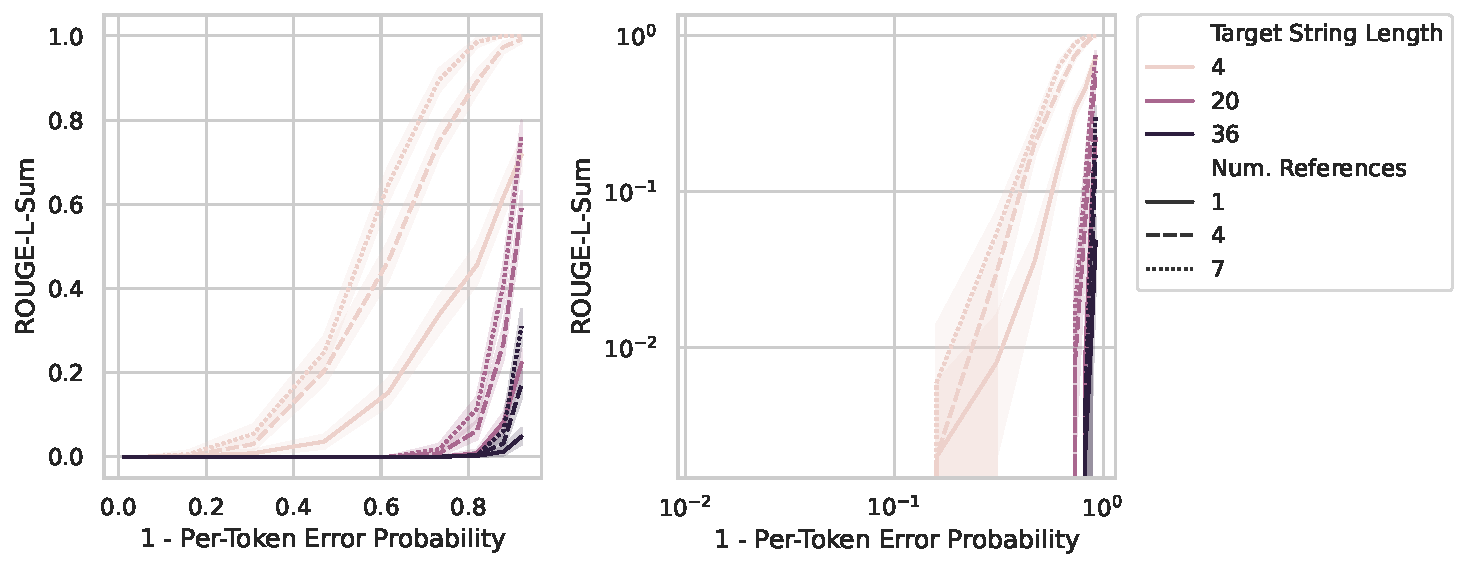
\includegraphics[width=0.95\textwidth]{figures/rouge_understanding/rougeLsum_vs_token_error_prob_scaling_simulation.pdf}
    \caption{\textbf{ROUGE-L-Sum is a sharp metric.} Simulations show that as the per-token error probability slightly increase (e.g. from 0.05 to 0.1), the ROUGE-L-Sum metric sharply falls.}
    \label{fig:app:metric_scaling:rougeLsum}
\end{figure}


Another BIG-Bench metric \cite{srivastava2022beyond} is ROUGE-L-Sum \cite{lin2004rouge}, a metric based on the longest common subsequence (LCS) between two sequences. Section 3.2 of \cite{lin2004rouge} gives the exact definition, but the key property is that ROUGE-L-Sum measures the ``union" LCS, which means ``stitching" together LCSs across the candidate and multiple references. As explained in the original paper: if the candidate sequence is $c = w_1 w_2 w_3 w_4 w_5$, and if there are two reference sequences $r_1 = w_1 w_2 w_6 w_7 w_8$ and $r_2 = w_1 w_3 w_8 w_9 w_5$, then $LCS(r_1, c) = w_1 w_2$ and $LCS(r_2, c) =w_1 w_3 w_5$, then the \textit{union} 
-LCS of $c, r_1, r_2$ is $w_1 w_2 w_3 w_5$, with length 4. Intuitively, this disproportionately benefits models with smaller error rates because their mistakes can be ``stitched" across multiple references; this is confirmed in simulation (Fig. \ref{fig:app:metric_scaling:rougeLsum}).


% \subsection{BLEU}
% \label{app:metric_scaling:bleu}


% \subsection{Emergence does not require on scaling laws: decreasing cross-entropy loss and stricter exact match is all you need }

% The goal of this section is to show that scaling laws are not necessary to create emergence and that many functional forms of the loss are valid as long as the form decreases as some other variable decreases -- say the number of parameters in the model.
% This typically holds in modern machine learning. 
% We do this by considering different functional forms of the cross entropy $CE(N)$, as a function of the number of parameters $N$, and show emergence, i.e. sharpness and unpredictability.
% We illustrate this by showing the programmer can exaggerate the sharpness (and therefore emergence) by implying increasing the exact number of tokens required to get correct in the accuracy, i.e. increasing $L$ in our notation.

% \subsubsection{Argument}

% Recall from section \ref{sec:alt_explanation} the accuracy requiring all $L$ tokens to be correct for a model of size $N$ as a function of cross-entropy $CE(N)$:

% \begin{equation*}
%     \text{Accuracy}(N) \approx p_N(\text{single token correct})^{\text{num. of tokens}} = \exp \Big(- CE(N) \Big)^L
% \end{equation*}

% We plot this equation using three functional forms for a decreasing cross-entropy loss in figure \ref{fig:decreasing_loss_leads_to_emergence_as_L_increases} for increasing values of $L$.
% These increasing values of $L$ induce a sharper -- therefore, seemingly more emergent curve when plotting the accuracy. 
% This means that if the programmer simply requires a stricter accuracy, he can make a perfectly smooth and predictable cross-entropy loss suddenly become sharp and unpredictable, i.e. ``emergent". 
% We show numerically it is independent of the functional form and instead that it only requires the cross-entropy to be decreasing and the accuracy metric to have some non-linear transformation that makes it sharper. 
% Therefore, if one had only tracked the cross-entropy loss instead, one could have had a smooth predictable curve for the models.
% This implies small-scale experimentation is still relevant, and we wish to highly that GPT-4 \cite{gpt4} small-scale experiment in conjunction with scaling loss. 
% We'd like to emphasize that changing the evaluation metric can suddenly induce emergence, and it is not an intrinsic property of the model. 

% %The goal will be to show that if $CE(N)$ decreases with different functional forms that $acc$ is emergent (either sharp or unpredictable).
% % TODO: sharp due to L
% % TODO: unpredictable due to constant and L

% \begin{figure}[htbp]
%   \centering
%   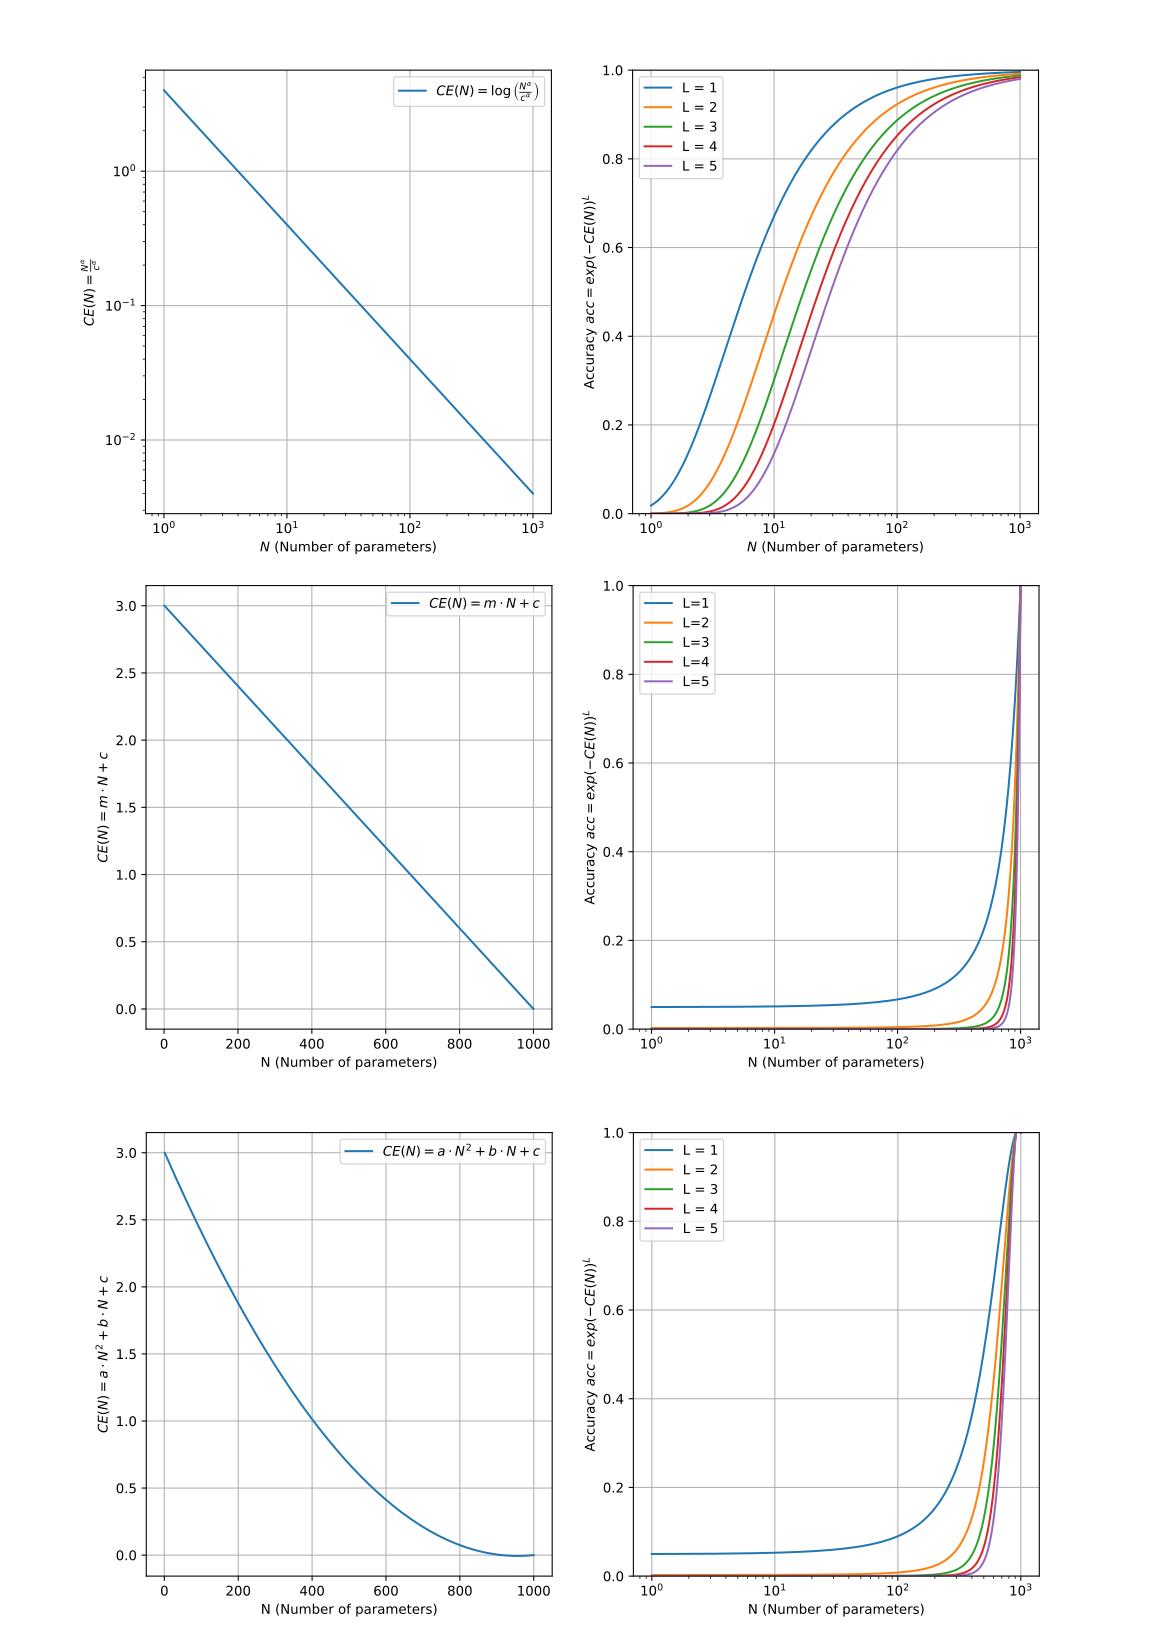
\includegraphics[width=0.8\textwidth]{figures/loss_decreasing_leads_to_emergence/decreasing_loss_leads_to_emergence_as_L_increases.png}
%   \caption{
%   \textbf{Emergence does not depend on scaling laws: any decreasing cross-entropy loss induces apparent emergence as L increases as you require more tokens to be exactly correct, i.e. L increases.}
%   The first row shows the same argument as in the main section, where a decreasing cross-entropy loss as a scaling law induces emergence as $L$ increases.
%   The second row shows the that apparent emergence is induced even when the cross-entropy loss decreases linearly.
%   The third row shows that the apparent emergence is induced when the cross-entropy loss decreases quadratically.
%   Emergence is amplified in this case especially by the increase in sharpness as more tokens are required to be correct. 
%   This means that simply changing the evaluation metric can suddenly induce emergence, and it is not an intrinsic property of the model. 
%   }
%   \label{fig:decreasing_loss_leads_to_emergence_as_L_increases}
% \end{figure}


\section{Inducing Emergent Abilities in Networks on Vision Tasks}
\label{app:sec:inducing_emergence_vision}

\subsection{Emergent Classification of MNIST Handwritten Digits by Convolutional Networks}

\begin{figure}
    \centering
    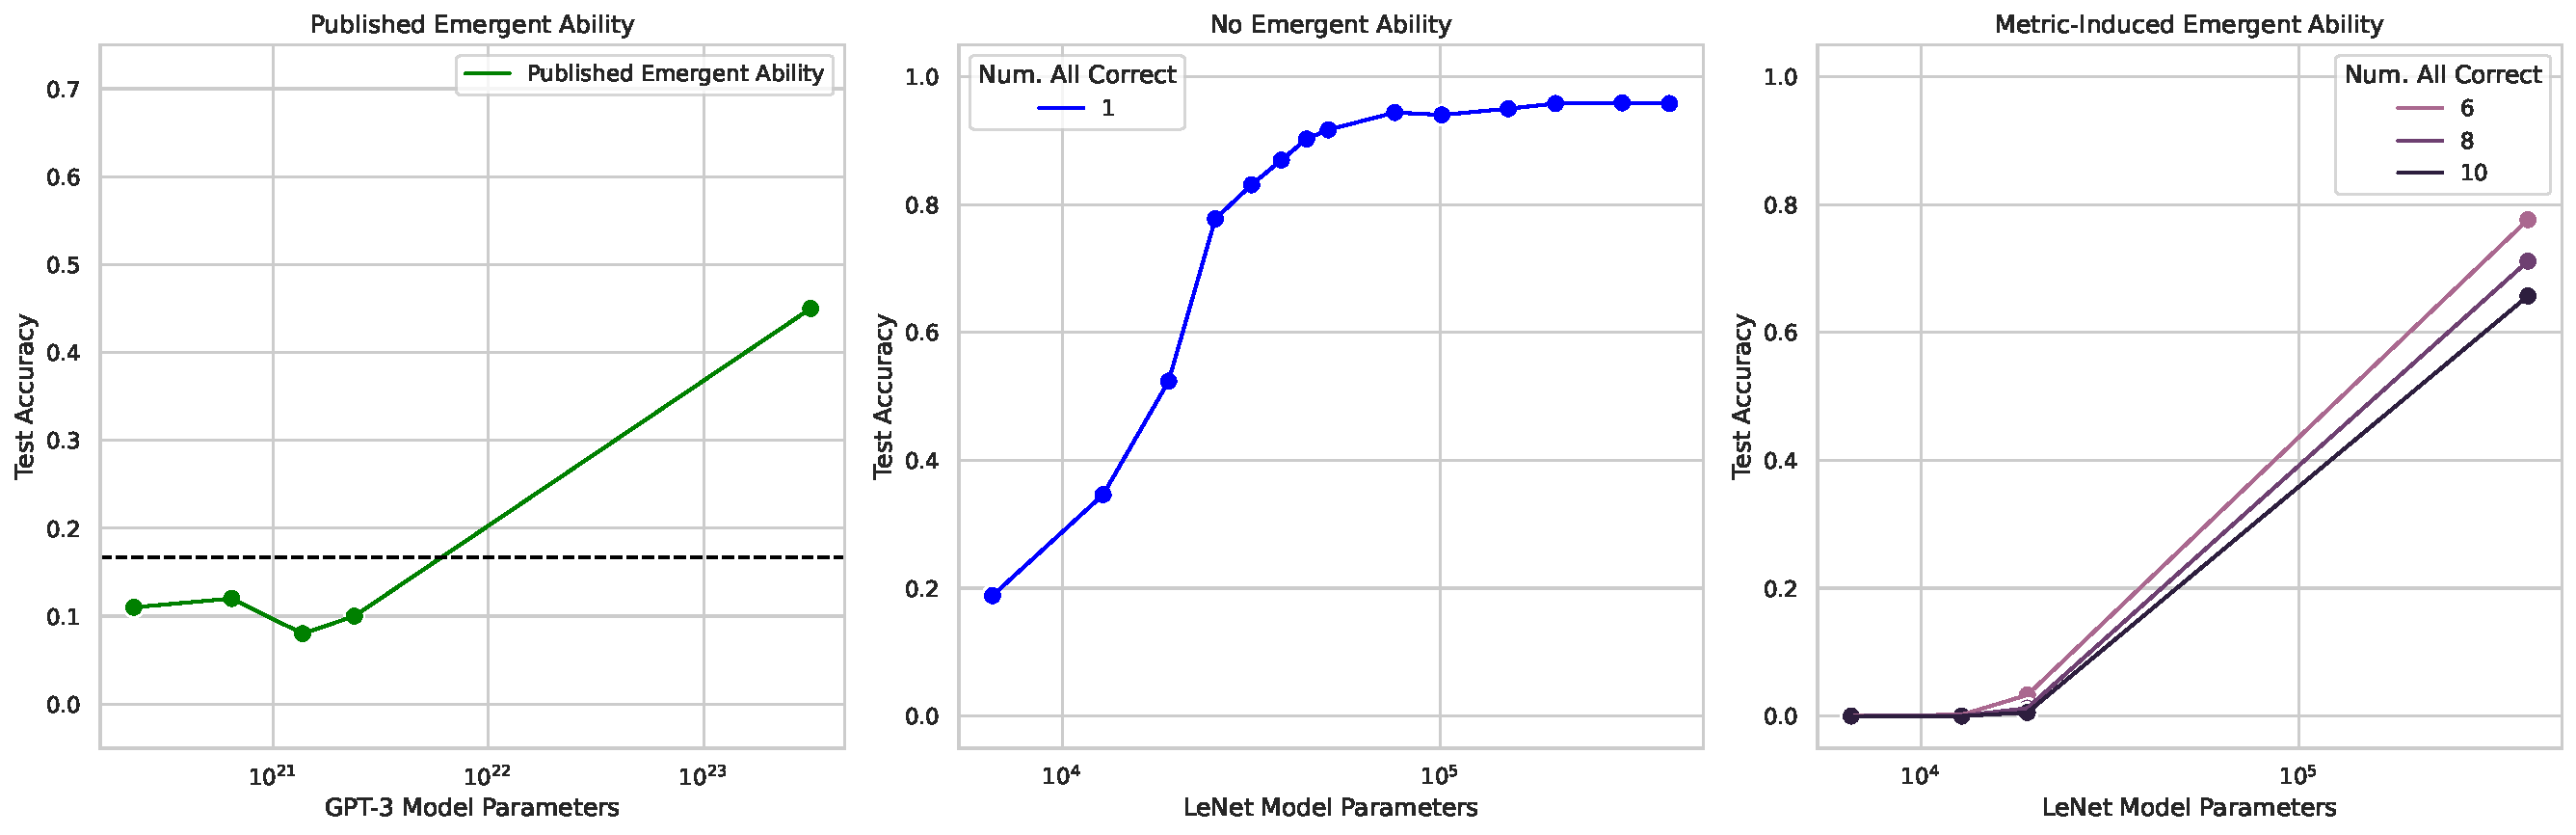
\includegraphics[width=\textwidth]{figures/vision/no_emergence_and_emergence_dataset=mnist.pdf}
    \caption{\textbf{Induced emergent MNIST classification ability in convolutional networks.} (A) A published emergent ability from the BIG-Bench Grounded Mappings task \cite{wei2022emergent}. (B) LeNet trained on MNIST \cite{lecun1998mnist} displays a predictable, commonplace sigmoidal increase in test accuracy as model parameters increase. (C) When accuracy is redefined as correctly classifying $K$ out of $K$ independent test data, this newly defined metric induces a seemingly unpredictable change.}
    \label{fig:vision_mnist}
\end{figure}

We begin by inducing an emergent classification ability in a LeNet convolutional neural network family \cite{lecun1998gradient}, trained on the MNIST handwritten digits dataset \cite{lecun1998mnist}.
This family displays smoothly increasing test accuracy as the number of parameters increase (Fig. \ref{fig:vision_mnist}B).
To emulate the accuracy metric used by emergence papers \cite{ganguli2022predictability, wei2022emergent, srivastava2022beyond}, we use \textit{subset accuracy}: 1 if the network classifies $K$ out of $K$ (independent) test data correctly, 0 otherwise.
Under this definition of accuracy, the model family displays an ``emergent" ability to correctly classify sets of MNIST digits as $K$ increases from $1$ to $5$, especially when combined with sparse sampling of model sizes (Fig. \ref{fig:vision_mnist}C).
This convolutional family's emergent classification ability qualitatively matches published emergent abilities, e.g., at the BIG-Bench Grounded Mappings task \cite{wei2022emergent} (Fig. \ref{fig:vision_mnist}A).

\fi

\subsection*{Acknowledgments}
We would like to thank
Yossi Arjevani,
Elad Eban,
Moritz Hardt,
Elad Hazan,
Percy Liang,
Nati Linial,
Ben Recht, and
Shai Shalev-Shwartz
for fruitful discussions, comments, and suggestions.

\bibliographystyle{plainnat}
\bibliography{bib}

\end{document}
